\documentclass[12pt]{report}

%%
% to enumerate subsubsection
%%
\addtocounter{tocdepth}{3}
\setcounter{secnumdepth}{3}
% \usepackage{tgtermes}
\usepackage[a4paper, margin=1in]{geometry}
\usepackage[T1]{fontenc}
\usepackage[utf8]{inputenc}
\usepackage{graphicx} 
\usepackage{tikz}
\usepackage{amsmath, amssymb}

%%
% to enumerate subsubsection
%%
\addtocounter{tocdepth}{3}
\setcounter{secnumdepth}{3}

% Snippet
\newcommand{\BSM}{Black--Scholes--Merton }
\newcommand{\lnorm}{log-normally }
\newcommand{\bmotion}{Brownian Motion }
\newcommand{\stvar}{stochastic variable }
\newcommand{\wienpro}{Wiener process }
\newcommand{\markpro}{Markov process }

% 
% Bunch of new commands
% 
% brownian motion
\newcommand{\dBm}{dW\left(t\right)}
\newcommand{\DBm}{\delta{W\left(t\right)}}
\newcommand{\Bm}{W\left(t\right)}
\newcommand{\Dt}{\Delta t} 
\newcommand{\Bmdist}{\DBm \sim N \left( 0, \Dt \right)}
\newcommand{\ft}{f\left(t, \Bm \right)}
\newcommand{\E}{\mathop{\mathbb{E}}}
\newcommand{\ct}{c\left(t, x\right)}
\newcommand{\dcx}{\frac{\delta\ct}{\delta x}}
\newcommand{\dciix}{\frac{\delta^2\ct}{\delta x^2}}
\newcommand{\dct}{\frac{\delta\ct}{\delta t}}
\newcommand{\N}[1]{N\left(#1\right)}
\newcommand{\dsub}[1]{d_{#1}\left(\Dt, x\right)}
\newcommand{\call}[2]{c\left( #1, #2\right)}
% % about stock
\newcommand{\St}{S\left(t\right)}
\newcommand{\Si}{S\left(0\right)}
\newcommand{\dSt}{dS\left(t\right)}
\newcommand{\DSt}{\Delta S\left(t\right)}
\newcommand{\dSr}{\frac{\dSt}{\St}}
\newcommand{\DSr}{\frac{\DSt}{\St}}
\newcommand{\Scontinuous}{\St = \Si e^{\sigma\Bm + \left(\alpha - \frac{1}{2 \sigma^2}\right)t}}
\newcommand{\Itobmdiff}{d\ft = \left[\frac{\partial \ft }{\partial t} + \frac{1}{2} \frac{\partial ^2\ft }{\partial x^2}\right]dt + \frac{\partial \ft}{\partial x} \dBm}
\newcommand{\Scontinousdiff}{d\St &= \alpha \St dt + \sigma \St \dBm}
\newcommand{\Scontinuousrate}{\dSr &= \alpha dt + \sigma \dBm}
 \newcommand{\Sdiscretediff}{d\St &= \alpha \St \Dt + \sigma \St \dBm}
\newcommand{\Sshort}{\Si e^{X}}
\newcommand{\CCRdist}{X \sim N\left(\left(\alpha - \frac{1}{2}\sigma^2\right)t, \sigma^2 t\right)}
\newcommand{\Sdiscreterate}{\DSr &= \alpha \Delta t + \sigma \DBm}
\newcommand{\Sdiscreterateexp}{\E \DSr = \alpha \Dt}
\newcommand{\Sdiscreteratevar}{var \DSr = \sigma ^2 \Dt}
\newcommand{\Sdiscreteratedist}{\DSr \sim N\left(\alpha\Dt, \sigma\Dt\right)}
\newcommand{\Sexp}{\E\St = \Si e^{\alpha t}}
\newcommand{\Svar}{var\St = \Si^2 e^{2\alpha t}\left(e^{\sigma^2 t} - 1\right)}
\newcommand{\Sshortt}{\St = \Si e^{X t}}
\newcommand{\CCRt}{X = \frac{1}{t} \ln{\frac{\St}{\Si}}}
\newcommand{\CCRtdist}{X \sim N\left(\alpha - \frac{\sigma^2}{2}, \frac{\sigma^2}{t}\right)}
\newcommand{\BSMpde}{\dct + r x \dcx + \frac{1}{2} \sigma^2 x^2 \dciix = r\ct}
\newcommand{\BSMeq}[1]{r\call{t}{#1} = \frac{\partial \call{t}{#1}}{\partial t} + r #1 \frac{\partial \call{t}{#1}}{\partial #1} + \frac{1}{2} \sigma ^2 #1 ^2 \frac{\partial ^2 \call{t}{#1}}{\partial #1 ^2}}
\newcommand{\BSMsol}{\ct = x\N{\dsub{+}} - K e^{-r\Dt} \N{\dsub{-}}}
\newcommand{\dpm}{\dsub{\pm} = \frac{1}{\sigma\sqrt{\Dt}} \left[\log\frac{x}{K} + \left(r \pm \frac{\sigma^2}{2}\Dt\right)\right]}

\usepackage{Sweave}
\begin{document}
\Sconcordance{concordance:index.tex:index.Rnw:%
1 18 1 1 0 13 1}
\Sconcordance{concordance:index.tex:./State/index.Rnw:ofs 33:%
1 55 1}
\Sconcordance{concordance:index.tex:index.Rnw:ofs 89:%
34 4 1}

\tableofcontents{}



%%%%%%%%%%%%%%%%%%%%%%%%%%%%%%%%%%%%%%%%%%%%%%%%%%%%%%%%%%%%%%%%%%%%%%%%%%%%%%%%
%
%  CHAPTER: Introduction
%
%%%%%%%%%%%%%%%%%%%%%%%%%%%%%%%%%%%%%%%%%%%%%%%%%%%%%%%%%%%%%%%%%%%%%%%%%%%%%%%%
\chapter*{Introduction}
\label{cha:Introduction}
\addcontentsline{toc}{chapter}{Introduction}
Talk about what is done to price a vanilla option throuhout the BSM method.
%\SweaveUTF8
%%%%%%%%%%%%%%%%%%%%%%%%%%%%%%%%%%%%%%%%%%%%%%%%%%%%%%%%%%%%%%%%%%%%%%%%%%%%%%%% 
%
%  CHAPTER:The underlying models
%
%%%%%%%%%%%%%%%%%%%%%%%%%%%%%%%%%%%%%%%%%%%%%%%%%%%%%%%%%%%%%%%%%%%%%%%%%%%%%%%%
\chapter{The underlying model}
\label{cha:underlying}
  


%%%%%%%%%%%%%%%%%%%%%%%%%%%%%%%%%%%%%%%%%%%%%%%%
% SECTION: Overview
%%%%%%%%%%%%%%%%%%%%%%%%%%%%%%%%%%%%%%%%%%%%%%%%
\section{Overview}
\label{sec:Overview}

This chapter highlights one specific model that is used to model the price ticker of a share of stock for any time $t$ in the future.

Equation (\ref{eq:Scontinuous}) features a stochastic process where the only random component is the Brownian motion $\Bm$.
The others parameters of (\ref{eq:Scontinuous}) are $\alpha$ and $\sigma$, which respectively are the mean rate of return and the volatility of a stock price whose path is described by that model.

\begin{center}
  \begin{equation}
    \Scontinuous
    \label{eq:Scontinuous}
  \end{equation}
\end{center}

 The condition underlying by (\ref{eq:Scontinuous}) is that the mean rate of return and the volatility of the stock price is constant. The path is continuous, there is no jump in the course of the stock price evolution. Moreover it will be shown in subsequent section that the stochastic process (\ref{eq:Scontinuous}) is log-normally distributed.

%%%%%%%%%%%%%%%%%%%%%%%%%%%%%%%%%%%%%%%%%%%%%%%%
% SECTION: Derivation
%%%%%%%%%%%%%%%%%%%%%%%%%%%%%%%%%%%%%%%%%%%%%%%%
\section{Derivation}
\label{sec:Derivation}

The equation (\ref{eq:Scontinuous}) could be derived using Itô's formula (\ref{eq:Itobmdiff}) in order to get the differential form of that equation. The provided differential formula will be next used to find out the first and second moments of the distribution underpinned by the stock price random process.

\begin{center}
  \begin{equation}
    \Itobmdiff \label{eq:Itobmdiff}
  \end{equation}
\end{center}

The term $d\ft$ in (\ref{eq:Itobmdiff}) represents any changes in the value of a function $\ft$ occuring over a infinitesimally small move in time $dt$. The related function is any one involving time along with a Brownian motion. For that matter in the present case, $ \ft = \St $.
By applying the tranformation inccured by Itô, the two following equations (\ref{eq:Scontinuousdiff}, \ref{eq:Scontinuousrate}) emerge:
 
\begin{center}
  \begin{subequations}
    \begin{align}
      \Scontinousdiff \label{eq:Scontinuousdiff} \\
      \Scontinuousrate \label{eq:Scontinuousrate}
    \end{align}
  \end{subequations}
\end{center}

In one hand, the equation (\ref{eq:Scontinuousdiff}) shows that any change occuring in the stock price over an small amount of time is due to one fully predictable element -- its drift rate ($\alpha \St$) -- and another one that brings uncertainty.

In the other hand, equation (\ref{eq:Scontinuousrate}) relates the rate of return of the stock price over a small amount of time. Because the uncertainty given is given by the Browinan motion has an expectation of zero, it could be shown that the mean rate of return of a stock price following the model (\ref{Scontinuous}) is equal to $\alpha$, as stated through (\ref{eq:return.s.dist}).

\begin{center}
  \begin{equation}
     \dSr \sim N(\mu dt, \sigma^2 t)
     \label{eq:return.s.dist}
  \end{equation}
\end{center}


The figure (\ref{plot:returnDensity}) shows that the normality expectation holds, for equation \ref{eq:return.s.dist}. The solid line exibits the normal distribution bell curve ($N \sim (0, 40 * 360^{-1}$)). While the bins represent the distribution of the increments from a stock processes, with parameters $\alpha = 0$, $\sigma = 40\%$ and $\Dt = 360^{-1}$.

 
\begin{figure}[!h]
\centering
% Created by tikzDevice version 0.11 on 2018-04-13 09:25:50
% !TEX encoding = UTF-8 Unicode
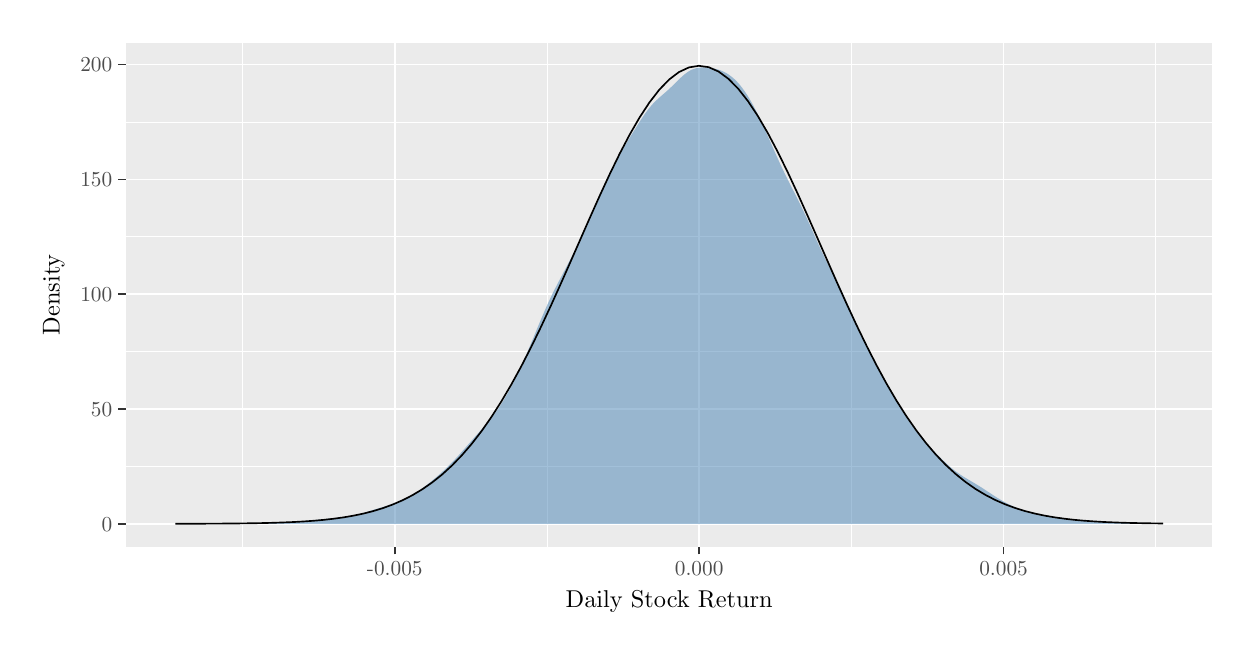
\begin{tikzpicture}[x=1pt,y=1pt]
\definecolor{fillColor}{RGB}{255,255,255}
\path[use as bounding box,fill=fillColor,fill opacity=0.00] (0,0) rectangle (433.62,216.81);
\begin{scope}
\path[clip] (  0.00,  0.00) rectangle (433.62,216.81);
\definecolor{drawColor}{RGB}{255,255,255}
\definecolor{fillColor}{RGB}{255,255,255}

\path[draw=drawColor,line width= 0.6pt,line join=round,line cap=round,fill=fillColor] (  0.00,  0.00) rectangle (433.62,216.81);
\end{scope}
\begin{scope}
\path[clip] ( 35.50, 29.26) rectangle (428.12,211.31);
\definecolor{fillColor}{gray}{0.92}

\path[fill=fillColor] ( 35.50, 29.26) rectangle (428.12,211.31);
\definecolor{drawColor}{RGB}{255,255,255}

\path[draw=drawColor,line width= 0.3pt,line join=round] ( 35.50, 58.28) --
	(428.12, 58.28);

\path[draw=drawColor,line width= 0.3pt,line join=round] ( 35.50, 99.76) --
	(428.12, 99.76);

\path[draw=drawColor,line width= 0.3pt,line join=round] ( 35.50,141.25) --
	(428.12,141.25);

\path[draw=drawColor,line width= 0.3pt,line join=round] ( 35.50,182.73) --
	(428.12,182.73);

\path[draw=drawColor,line width= 0.3pt,line join=round] ( 77.67, 29.26) --
	( 77.67,211.31);

\path[draw=drawColor,line width= 0.3pt,line join=round] (187.65, 29.26) --
	(187.65,211.31);

\path[draw=drawColor,line width= 0.3pt,line join=round] (297.64, 29.26) --
	(297.64,211.31);

\path[draw=drawColor,line width= 0.3pt,line join=round] (407.62, 29.26) --
	(407.62,211.31);

\path[draw=drawColor,line width= 0.6pt,line join=round] ( 35.50, 37.53) --
	(428.12, 37.53);

\path[draw=drawColor,line width= 0.6pt,line join=round] ( 35.50, 79.02) --
	(428.12, 79.02);

\path[draw=drawColor,line width= 0.6pt,line join=round] ( 35.50,120.50) --
	(428.12,120.50);

\path[draw=drawColor,line width= 0.6pt,line join=round] ( 35.50,161.99) --
	(428.12,161.99);

\path[draw=drawColor,line width= 0.6pt,line join=round] ( 35.50,203.47) --
	(428.12,203.47);

\path[draw=drawColor,line width= 0.6pt,line join=round] (132.66, 29.26) --
	(132.66,211.31);

\path[draw=drawColor,line width= 0.6pt,line join=round] (242.64, 29.26) --
	(242.64,211.31);

\path[draw=drawColor,line width= 0.6pt,line join=round] (352.63, 29.26) --
	(352.63,211.31);
\definecolor{fillColor}{RGB}{70,130,180}

\path[fill=fillColor,fill opacity=0.50] ( 53.35, 37.57) --
	( 54.05, 37.57) --
	( 54.75, 37.57) --
	( 55.44, 37.57) --
	( 56.14, 37.57) --
	( 56.84, 37.56) --
	( 57.54, 37.56) --
	( 58.24, 37.56) --
	( 58.94, 37.55) --
	( 59.63, 37.55) --
	( 60.33, 37.55) --
	( 61.03, 37.54) --
	( 61.73, 37.54) --
	( 62.43, 37.54) --
	( 63.13, 37.54) --
	( 63.83, 37.54) --
	( 64.52, 37.54) --
	( 65.22, 37.54) --
	( 65.92, 37.54) --
	( 66.62, 37.55) --
	( 67.32, 37.55) --
	( 68.02, 37.56) --
	( 68.71, 37.56) --
	( 69.41, 37.57) --
	( 70.11, 37.58) --
	( 70.81, 37.58) --
	( 71.51, 37.59) --
	( 72.21, 37.61) --
	( 72.91, 37.62) --
	( 73.60, 37.63) --
	( 74.30, 37.64) --
	( 75.00, 37.66) --
	( 75.70, 37.67) --
	( 76.40, 37.69) --
	( 77.10, 37.70) --
	( 77.80, 37.71) --
	( 78.49, 37.73) --
	( 79.19, 37.74) --
	( 79.89, 37.75) --
	( 80.59, 37.76) --
	( 81.29, 37.77) --
	( 81.99, 37.78) --
	( 82.68, 37.78) --
	( 83.38, 37.79) --
	( 84.08, 37.80) --
	( 84.78, 37.81) --
	( 85.48, 37.81) --
	( 86.18, 37.82) --
	( 86.88, 37.83) --
	( 87.57, 37.85) --
	( 88.27, 37.86) --
	( 88.97, 37.88) --
	( 89.67, 37.90) --
	( 90.37, 37.92) --
	( 91.07, 37.94) --
	( 91.76, 37.97) --
	( 92.46, 38.00) --
	( 93.16, 38.03) --
	( 93.86, 38.07) --
	( 94.56, 38.10) --
	( 95.26, 38.15) --
	( 95.96, 38.19) --
	( 96.65, 38.24) --
	( 97.35, 38.29) --
	( 98.05, 38.34) --
	( 98.75, 38.40) --
	( 99.45, 38.46) --
	(100.15, 38.52) --
	(100.85, 38.58) --
	(101.54, 38.64) --
	(102.24, 38.71) --
	(102.94, 38.77) --
	(103.64, 38.84) --
	(104.34, 38.91) --
	(105.04, 38.99) --
	(105.73, 39.06) --
	(106.43, 39.14) --
	(107.13, 39.22) --
	(107.83, 39.30) --
	(108.53, 39.38) --
	(109.23, 39.45) --
	(109.93, 39.53) --
	(110.62, 39.60) --
	(111.32, 39.67) --
	(112.02, 39.74) --
	(112.72, 39.81) --
	(113.42, 39.88) --
	(114.12, 39.95) --
	(114.81, 40.03) --
	(115.51, 40.12) --
	(116.21, 40.22) --
	(116.91, 40.33) --
	(117.61, 40.47) --
	(118.31, 40.61) --
	(119.01, 40.77) --
	(119.70, 40.95) --
	(120.40, 41.15) --
	(121.10, 41.35) --
	(121.80, 41.56) --
	(122.50, 41.78) --
	(123.20, 42.01) --
	(123.90, 42.23) --
	(124.59, 42.45) --
	(125.29, 42.67) --
	(125.99, 42.89) --
	(126.69, 43.10) --
	(127.39, 43.31) --
	(128.09, 43.51) --
	(128.78, 43.71) --
	(129.48, 43.92) --
	(130.18, 44.13) --
	(130.88, 44.35) --
	(131.58, 44.57) --
	(132.28, 44.81) --
	(132.98, 45.06) --
	(133.67, 45.33) --
	(134.37, 45.61) --
	(135.07, 45.91) --
	(135.77, 46.22) --
	(136.47, 46.56) --
	(137.17, 46.91) --
	(137.86, 47.29) --
	(138.56, 47.69) --
	(139.26, 48.11) --
	(139.96, 48.54) --
	(140.66, 49.00) --
	(141.36, 49.48) --
	(142.06, 49.97) --
	(142.75, 50.48) --
	(143.45, 51.00) --
	(144.15, 51.53) --
	(144.85, 52.08) --
	(145.55, 52.64) --
	(146.25, 53.21) --
	(146.95, 53.78) --
	(147.64, 54.37) --
	(148.34, 54.98) --
	(149.04, 55.59) --
	(149.74, 56.22) --
	(150.44, 56.86) --
	(151.14, 57.52) --
	(151.83, 58.20) --
	(152.53, 58.89) --
	(153.23, 59.60) --
	(153.93, 60.33) --
	(154.63, 61.08) --
	(155.33, 61.83) --
	(156.03, 62.60) --
	(156.72, 63.38) --
	(157.42, 64.17) --
	(158.12, 64.96) --
	(158.82, 65.76) --
	(159.52, 66.56) --
	(160.22, 67.36) --
	(160.91, 68.15) --
	(161.61, 68.95) --
	(162.31, 69.74) --
	(163.01, 70.52) --
	(163.71, 71.31) --
	(164.41, 72.10) --
	(165.11, 72.90) --
	(165.80, 73.70) --
	(166.50, 74.52) --
	(167.20, 75.37) --
	(167.90, 76.25) --
	(168.60, 77.16) --
	(169.30, 78.11) --
	(170.00, 79.10) --
	(170.69, 80.15) --
	(171.39, 81.24) --
	(172.09, 82.37) --
	(172.79, 83.56) --
	(173.49, 84.80) --
	(174.19, 86.09) --
	(174.88, 87.42) --
	(175.58, 88.80) --
	(176.28, 90.21) --
	(176.98, 91.66) --
	(177.68, 93.15) --
	(178.38, 94.66) --
	(179.08, 96.21) --
	(179.77, 97.79) --
	(180.47, 99.40) --
	(181.17,101.03) --
	(181.87,102.68) --
	(182.57,104.35) --
	(183.27,106.04) --
	(183.96,107.73) --
	(184.66,109.42) --
	(185.36,111.10) --
	(186.06,112.75) --
	(186.76,114.38) --
	(187.46,115.97) --
	(188.16,117.52) --
	(188.85,119.02) --
	(189.55,120.48) --
	(190.25,121.89) --
	(190.95,123.27) --
	(191.65,124.62) --
	(192.35,125.95) --
	(193.05,127.27) --
	(193.74,128.59) --
	(194.44,129.92) --
	(195.14,131.25) --
	(195.84,132.60) --
	(196.54,133.96) --
	(197.24,135.35) --
	(197.93,136.75) --
	(198.63,138.18) --
	(199.33,139.62) --
	(200.03,141.09) --
	(200.73,142.59) --
	(201.43,144.11) --
	(202.13,145.65) --
	(202.82,147.23) --
	(203.52,148.83) --
	(204.22,150.45) --
	(204.92,152.09) --
	(205.62,153.74) --
	(206.32,155.38) --
	(207.01,157.02) --
	(207.71,158.63) --
	(208.41,160.22) --
	(209.11,161.76) --
	(209.81,163.27) --
	(210.51,164.72) --
	(211.21,166.11) --
	(211.90,167.46) --
	(212.60,168.75) --
	(213.30,170.00) --
	(214.00,171.22) --
	(214.70,172.40) --
	(215.40,173.56) --
	(216.10,174.70) --
	(216.79,175.84) --
	(217.49,176.97) --
	(218.19,178.10) --
	(218.89,179.22) --
	(219.59,180.35) --
	(220.29,181.47) --
	(220.98,182.57) --
	(221.68,183.65) --
	(222.38,184.71) --
	(223.08,185.72) --
	(223.78,186.69) --
	(224.48,187.60) --
	(225.18,188.44) --
	(225.87,189.23) --
	(226.57,189.96) --
	(227.27,190.64) --
	(227.97,191.29) --
	(228.67,191.90) --
	(229.37,192.51) --
	(230.06,193.11) --
	(230.76,193.72) --
	(231.46,194.34) --
	(232.16,194.99) --
	(232.86,195.66) --
	(233.56,196.34) --
	(234.26,197.04) --
	(234.95,197.73) --
	(235.65,198.41) --
	(236.35,199.06) --
	(237.05,199.67) --
	(237.75,200.24) --
	(238.45,200.75) --
	(239.15,201.19) --
	(239.84,201.56) --
	(240.54,201.85) --
	(241.24,202.08) --
	(241.94,202.25) --
	(242.64,202.36) --
	(243.34,202.42) --
	(244.03,202.44) --
	(244.73,202.43) --
	(245.43,202.39) --
	(246.13,202.32) --
	(246.83,202.24) --
	(247.53,202.12) --
	(248.23,201.99) --
	(248.92,201.82) --
	(249.62,201.62) --
	(250.32,201.38) --
	(251.02,201.11) --
	(251.72,200.78) --
	(252.42,200.41) --
	(253.11,199.99) --
	(253.81,199.50) --
	(254.51,198.96) --
	(255.21,198.36) --
	(255.91,197.69) --
	(256.61,196.96) --
	(257.31,196.16) --
	(258.00,195.29) --
	(258.70,194.35) --
	(259.40,193.35) --
	(260.10,192.28) --
	(260.80,191.14) --
	(261.50,189.94) --
	(262.20,188.68) --
	(262.89,187.36) --
	(263.59,185.99) --
	(264.29,184.57) --
	(264.99,183.10) --
	(265.69,181.60) --
	(266.39,180.05) --
	(267.08,178.49) --
	(267.78,176.90) --
	(268.48,175.30) --
	(269.18,173.70) --
	(269.88,172.11) --
	(270.58,170.53) --
	(271.28,168.98) --
	(271.97,167.45) --
	(272.67,165.96) --
	(273.37,164.50) --
	(274.07,163.07) --
	(274.77,161.66) --
	(275.47,160.27) --
	(276.16,158.90) --
	(276.86,157.53) --
	(277.56,156.16) --
	(278.26,154.77) --
	(278.96,153.37) --
	(279.66,151.94) --
	(280.36,150.48) --
	(281.05,148.99) --
	(281.75,147.47) --
	(282.45,145.93) --
	(283.15,144.36) --
	(283.85,142.78) --
	(284.55,141.20) --
	(285.25,139.62) --
	(285.94,138.07) --
	(286.64,136.55) --
	(287.34,135.06) --
	(288.04,133.61) --
	(288.74,132.19) --
	(289.44,130.81) --
	(290.13,129.45) --
	(290.83,128.11) --
	(291.53,126.76) --
	(292.23,125.41) --
	(292.93,124.03) --
	(293.63,122.63) --
	(294.33,121.18) --
	(295.02,119.70) --
	(295.72,118.17) --
	(296.42,116.62) --
	(297.12,115.03) --
	(297.82,113.42) --
	(298.52,111.80) --
	(299.21,110.18) --
	(299.91,108.58) --
	(300.61,106.99) --
	(301.31,105.43) --
	(302.01,103.90) --
	(302.71,102.40) --
	(303.41,100.94) --
	(304.10, 99.52) --
	(304.80, 98.13) --
	(305.50, 96.78) --
	(306.20, 95.46) --
	(306.90, 94.17) --
	(307.60, 92.90) --
	(308.30, 91.65) --
	(308.99, 90.41) --
	(309.69, 89.19) --
	(310.39, 87.98) --
	(311.09, 86.78) --
	(311.79, 85.58) --
	(312.49, 84.39) --
	(313.18, 83.20) --
	(313.88, 82.01) --
	(314.58, 80.84) --
	(315.28, 79.67) --
	(315.98, 78.52) --
	(316.68, 77.38) --
	(317.38, 76.26) --
	(318.07, 75.18) --
	(318.77, 74.12) --
	(319.47, 73.10) --
	(320.17, 72.12) --
	(320.87, 71.18) --
	(321.57, 70.28) --
	(322.26, 69.41) --
	(322.96, 68.58) --
	(323.66, 67.78) --
	(324.36, 67.01) --
	(325.06, 66.25) --
	(325.76, 65.51) --
	(326.46, 64.79) --
	(327.15, 64.07) --
	(327.85, 63.36) --
	(328.55, 62.66) --
	(329.25, 61.96) --
	(329.95, 61.27) --
	(330.65, 60.58) --
	(331.35, 59.91) --
	(332.04, 59.26) --
	(332.74, 58.62) --
	(333.44, 58.01) --
	(334.14, 57.42) --
	(334.84, 56.86) --
	(335.54, 56.33) --
	(336.23, 55.83) --
	(336.93, 55.35) --
	(337.63, 54.89) --
	(338.33, 54.46) --
	(339.03, 54.03) --
	(339.73, 53.62) --
	(340.43, 53.21) --
	(341.12, 52.80) --
	(341.82, 52.39) --
	(342.52, 51.97) --
	(343.22, 51.55) --
	(343.92, 51.12) --
	(344.62, 50.68) --
	(345.31, 50.23) --
	(346.01, 49.77) --
	(346.71, 49.31) --
	(347.41, 48.85) --
	(348.11, 48.39) --
	(348.81, 47.93) --
	(349.51, 47.48) --
	(350.20, 47.04) --
	(350.90, 46.60) --
	(351.60, 46.18) --
	(352.30, 45.78) --
	(353.00, 45.38) --
	(353.70, 45.01) --
	(354.39, 44.65) --
	(355.09, 44.31) --
	(355.79, 43.98) --
	(356.49, 43.67) --
	(357.19, 43.37) --
	(357.89, 43.09) --
	(358.59, 42.82) --
	(359.28, 42.56) --
	(359.98, 42.32) --
	(360.68, 42.10) --
	(361.38, 41.88) --
	(362.08, 41.68) --
	(362.78, 41.50) --
	(363.48, 41.32) --
	(364.17, 41.16) --
	(364.87, 41.01) --
	(365.57, 40.86) --
	(366.27, 40.73) --
	(366.97, 40.60) --
	(367.67, 40.48) --
	(368.36, 40.36) --
	(369.06, 40.25) --
	(369.76, 40.15) --
	(370.46, 40.05) --
	(371.16, 39.95) --
	(371.86, 39.85) --
	(372.56, 39.76) --
	(373.25, 39.67) --
	(373.95, 39.58) --
	(374.65, 39.49) --
	(375.35, 39.40) --
	(376.05, 39.32) --
	(376.75, 39.23) --
	(377.44, 39.15) --
	(378.14, 39.06) --
	(378.84, 38.98) --
	(379.54, 38.90) --
	(380.24, 38.82) --
	(380.94, 38.74) --
	(381.64, 38.66) --
	(382.33, 38.59) --
	(383.03, 38.53) --
	(383.73, 38.46) --
	(384.43, 38.40) --
	(385.13, 38.35) --
	(385.83, 38.29) --
	(386.53, 38.25) --
	(387.22, 38.20) --
	(387.92, 38.16) --
	(388.62, 38.12) --
	(389.32, 38.08) --
	(390.02, 38.04) --
	(390.72, 38.01) --
	(391.41, 37.98) --
	(392.11, 37.95) --
	(392.81, 37.93) --
	(393.51, 37.90) --
	(394.21, 37.89) --
	(394.91, 37.87) --
	(395.61, 37.86) --
	(396.30, 37.85) --
	(397.00, 37.84) --
	(397.70, 37.84) --
	(398.40, 37.83) --
	(399.10, 37.83) --
	(399.80, 37.83) --
	(400.49, 37.83) --
	(401.19, 37.83) --
	(401.89, 37.83) --
	(402.59, 37.82) --
	(403.29, 37.82) --
	(403.99, 37.81) --
	(404.69, 37.80) --
	(405.38, 37.79) --
	(406.08, 37.78) --
	(406.78, 37.76) --
	(407.48, 37.75) --
	(408.18, 37.73) --
	(408.88, 37.72) --
	(409.58, 37.70) --
	(410.27, 37.69) --
	(410.27, 37.53) --
	(409.58, 37.53) --
	(408.88, 37.53) --
	(408.18, 37.53) --
	(407.48, 37.53) --
	(406.78, 37.53) --
	(406.08, 37.53) --
	(405.38, 37.53) --
	(404.69, 37.53) --
	(403.99, 37.53) --
	(403.29, 37.53) --
	(402.59, 37.53) --
	(401.89, 37.53) --
	(401.19, 37.53) --
	(400.49, 37.53) --
	(399.80, 37.53) --
	(399.10, 37.53) --
	(398.40, 37.53) --
	(397.70, 37.53) --
	(397.00, 37.53) --
	(396.30, 37.53) --
	(395.61, 37.53) --
	(394.91, 37.53) --
	(394.21, 37.53) --
	(393.51, 37.53) --
	(392.81, 37.53) --
	(392.11, 37.53) --
	(391.41, 37.53) --
	(390.72, 37.53) --
	(390.02, 37.53) --
	(389.32, 37.53) --
	(388.62, 37.53) --
	(387.92, 37.53) --
	(387.22, 37.53) --
	(386.53, 37.53) --
	(385.83, 37.53) --
	(385.13, 37.53) --
	(384.43, 37.53) --
	(383.73, 37.53) --
	(383.03, 37.53) --
	(382.33, 37.53) --
	(381.64, 37.53) --
	(380.94, 37.53) --
	(380.24, 37.53) --
	(379.54, 37.53) --
	(378.84, 37.53) --
	(378.14, 37.53) --
	(377.44, 37.53) --
	(376.75, 37.53) --
	(376.05, 37.53) --
	(375.35, 37.53) --
	(374.65, 37.53) --
	(373.95, 37.53) --
	(373.25, 37.53) --
	(372.56, 37.53) --
	(371.86, 37.53) --
	(371.16, 37.53) --
	(370.46, 37.53) --
	(369.76, 37.53) --
	(369.06, 37.53) --
	(368.36, 37.53) --
	(367.67, 37.53) --
	(366.97, 37.53) --
	(366.27, 37.53) --
	(365.57, 37.53) --
	(364.87, 37.53) --
	(364.17, 37.53) --
	(363.48, 37.53) --
	(362.78, 37.53) --
	(362.08, 37.53) --
	(361.38, 37.53) --
	(360.68, 37.53) --
	(359.98, 37.53) --
	(359.28, 37.53) --
	(358.59, 37.53) --
	(357.89, 37.53) --
	(357.19, 37.53) --
	(356.49, 37.53) --
	(355.79, 37.53) --
	(355.09, 37.53) --
	(354.39, 37.53) --
	(353.70, 37.53) --
	(353.00, 37.53) --
	(352.30, 37.53) --
	(351.60, 37.53) --
	(350.90, 37.53) --
	(350.20, 37.53) --
	(349.51, 37.53) --
	(348.81, 37.53) --
	(348.11, 37.53) --
	(347.41, 37.53) --
	(346.71, 37.53) --
	(346.01, 37.53) --
	(345.31, 37.53) --
	(344.62, 37.53) --
	(343.92, 37.53) --
	(343.22, 37.53) --
	(342.52, 37.53) --
	(341.82, 37.53) --
	(341.12, 37.53) --
	(340.43, 37.53) --
	(339.73, 37.53) --
	(339.03, 37.53) --
	(338.33, 37.53) --
	(337.63, 37.53) --
	(336.93, 37.53) --
	(336.23, 37.53) --
	(335.54, 37.53) --
	(334.84, 37.53) --
	(334.14, 37.53) --
	(333.44, 37.53) --
	(332.74, 37.53) --
	(332.04, 37.53) --
	(331.35, 37.53) --
	(330.65, 37.53) --
	(329.95, 37.53) --
	(329.25, 37.53) --
	(328.55, 37.53) --
	(327.85, 37.53) --
	(327.15, 37.53) --
	(326.46, 37.53) --
	(325.76, 37.53) --
	(325.06, 37.53) --
	(324.36, 37.53) --
	(323.66, 37.53) --
	(322.96, 37.53) --
	(322.26, 37.53) --
	(321.57, 37.53) --
	(320.87, 37.53) --
	(320.17, 37.53) --
	(319.47, 37.53) --
	(318.77, 37.53) --
	(318.07, 37.53) --
	(317.38, 37.53) --
	(316.68, 37.53) --
	(315.98, 37.53) --
	(315.28, 37.53) --
	(314.58, 37.53) --
	(313.88, 37.53) --
	(313.18, 37.53) --
	(312.49, 37.53) --
	(311.79, 37.53) --
	(311.09, 37.53) --
	(310.39, 37.53) --
	(309.69, 37.53) --
	(308.99, 37.53) --
	(308.30, 37.53) --
	(307.60, 37.53) --
	(306.90, 37.53) --
	(306.20, 37.53) --
	(305.50, 37.53) --
	(304.80, 37.53) --
	(304.10, 37.53) --
	(303.41, 37.53) --
	(302.71, 37.53) --
	(302.01, 37.53) --
	(301.31, 37.53) --
	(300.61, 37.53) --
	(299.91, 37.53) --
	(299.21, 37.53) --
	(298.52, 37.53) --
	(297.82, 37.53) --
	(297.12, 37.53) --
	(296.42, 37.53) --
	(295.72, 37.53) --
	(295.02, 37.53) --
	(294.33, 37.53) --
	(293.63, 37.53) --
	(292.93, 37.53) --
	(292.23, 37.53) --
	(291.53, 37.53) --
	(290.83, 37.53) --
	(290.13, 37.53) --
	(289.44, 37.53) --
	(288.74, 37.53) --
	(288.04, 37.53) --
	(287.34, 37.53) --
	(286.64, 37.53) --
	(285.94, 37.53) --
	(285.25, 37.53) --
	(284.55, 37.53) --
	(283.85, 37.53) --
	(283.15, 37.53) --
	(282.45, 37.53) --
	(281.75, 37.53) --
	(281.05, 37.53) --
	(280.36, 37.53) --
	(279.66, 37.53) --
	(278.96, 37.53) --
	(278.26, 37.53) --
	(277.56, 37.53) --
	(276.86, 37.53) --
	(276.16, 37.53) --
	(275.47, 37.53) --
	(274.77, 37.53) --
	(274.07, 37.53) --
	(273.37, 37.53) --
	(272.67, 37.53) --
	(271.97, 37.53) --
	(271.28, 37.53) --
	(270.58, 37.53) --
	(269.88, 37.53) --
	(269.18, 37.53) --
	(268.48, 37.53) --
	(267.78, 37.53) --
	(267.08, 37.53) --
	(266.39, 37.53) --
	(265.69, 37.53) --
	(264.99, 37.53) --
	(264.29, 37.53) --
	(263.59, 37.53) --
	(262.89, 37.53) --
	(262.20, 37.53) --
	(261.50, 37.53) --
	(260.80, 37.53) --
	(260.10, 37.53) --
	(259.40, 37.53) --
	(258.70, 37.53) --
	(258.00, 37.53) --
	(257.31, 37.53) --
	(256.61, 37.53) --
	(255.91, 37.53) --
	(255.21, 37.53) --
	(254.51, 37.53) --
	(253.81, 37.53) --
	(253.11, 37.53) --
	(252.42, 37.53) --
	(251.72, 37.53) --
	(251.02, 37.53) --
	(250.32, 37.53) --
	(249.62, 37.53) --
	(248.92, 37.53) --
	(248.23, 37.53) --
	(247.53, 37.53) --
	(246.83, 37.53) --
	(246.13, 37.53) --
	(245.43, 37.53) --
	(244.73, 37.53) --
	(244.03, 37.53) --
	(243.34, 37.53) --
	(242.64, 37.53) --
	(241.94, 37.53) --
	(241.24, 37.53) --
	(240.54, 37.53) --
	(239.84, 37.53) --
	(239.15, 37.53) --
	(238.45, 37.53) --
	(237.75, 37.53) --
	(237.05, 37.53) --
	(236.35, 37.53) --
	(235.65, 37.53) --
	(234.95, 37.53) --
	(234.26, 37.53) --
	(233.56, 37.53) --
	(232.86, 37.53) --
	(232.16, 37.53) --
	(231.46, 37.53) --
	(230.76, 37.53) --
	(230.06, 37.53) --
	(229.37, 37.53) --
	(228.67, 37.53) --
	(227.97, 37.53) --
	(227.27, 37.53) --
	(226.57, 37.53) --
	(225.87, 37.53) --
	(225.18, 37.53) --
	(224.48, 37.53) --
	(223.78, 37.53) --
	(223.08, 37.53) --
	(222.38, 37.53) --
	(221.68, 37.53) --
	(220.98, 37.53) --
	(220.29, 37.53) --
	(219.59, 37.53) --
	(218.89, 37.53) --
	(218.19, 37.53) --
	(217.49, 37.53) --
	(216.79, 37.53) --
	(216.10, 37.53) --
	(215.40, 37.53) --
	(214.70, 37.53) --
	(214.00, 37.53) --
	(213.30, 37.53) --
	(212.60, 37.53) --
	(211.90, 37.53) --
	(211.21, 37.53) --
	(210.51, 37.53) --
	(209.81, 37.53) --
	(209.11, 37.53) --
	(208.41, 37.53) --
	(207.71, 37.53) --
	(207.01, 37.53) --
	(206.32, 37.53) --
	(205.62, 37.53) --
	(204.92, 37.53) --
	(204.22, 37.53) --
	(203.52, 37.53) --
	(202.82, 37.53) --
	(202.13, 37.53) --
	(201.43, 37.53) --
	(200.73, 37.53) --
	(200.03, 37.53) --
	(199.33, 37.53) --
	(198.63, 37.53) --
	(197.93, 37.53) --
	(197.24, 37.53) --
	(196.54, 37.53) --
	(195.84, 37.53) --
	(195.14, 37.53) --
	(194.44, 37.53) --
	(193.74, 37.53) --
	(193.05, 37.53) --
	(192.35, 37.53) --
	(191.65, 37.53) --
	(190.95, 37.53) --
	(190.25, 37.53) --
	(189.55, 37.53) --
	(188.85, 37.53) --
	(188.16, 37.53) --
	(187.46, 37.53) --
	(186.76, 37.53) --
	(186.06, 37.53) --
	(185.36, 37.53) --
	(184.66, 37.53) --
	(183.96, 37.53) --
	(183.27, 37.53) --
	(182.57, 37.53) --
	(181.87, 37.53) --
	(181.17, 37.53) --
	(180.47, 37.53) --
	(179.77, 37.53) --
	(179.08, 37.53) --
	(178.38, 37.53) --
	(177.68, 37.53) --
	(176.98, 37.53) --
	(176.28, 37.53) --
	(175.58, 37.53) --
	(174.88, 37.53) --
	(174.19, 37.53) --
	(173.49, 37.53) --
	(172.79, 37.53) --
	(172.09, 37.53) --
	(171.39, 37.53) --
	(170.69, 37.53) --
	(170.00, 37.53) --
	(169.30, 37.53) --
	(168.60, 37.53) --
	(167.90, 37.53) --
	(167.20, 37.53) --
	(166.50, 37.53) --
	(165.80, 37.53) --
	(165.11, 37.53) --
	(164.41, 37.53) --
	(163.71, 37.53) --
	(163.01, 37.53) --
	(162.31, 37.53) --
	(161.61, 37.53) --
	(160.91, 37.53) --
	(160.22, 37.53) --
	(159.52, 37.53) --
	(158.82, 37.53) --
	(158.12, 37.53) --
	(157.42, 37.53) --
	(156.72, 37.53) --
	(156.03, 37.53) --
	(155.33, 37.53) --
	(154.63, 37.53) --
	(153.93, 37.53) --
	(153.23, 37.53) --
	(152.53, 37.53) --
	(151.83, 37.53) --
	(151.14, 37.53) --
	(150.44, 37.53) --
	(149.74, 37.53) --
	(149.04, 37.53) --
	(148.34, 37.53) --
	(147.64, 37.53) --
	(146.95, 37.53) --
	(146.25, 37.53) --
	(145.55, 37.53) --
	(144.85, 37.53) --
	(144.15, 37.53) --
	(143.45, 37.53) --
	(142.75, 37.53) --
	(142.06, 37.53) --
	(141.36, 37.53) --
	(140.66, 37.53) --
	(139.96, 37.53) --
	(139.26, 37.53) --
	(138.56, 37.53) --
	(137.86, 37.53) --
	(137.17, 37.53) --
	(136.47, 37.53) --
	(135.77, 37.53) --
	(135.07, 37.53) --
	(134.37, 37.53) --
	(133.67, 37.53) --
	(132.98, 37.53) --
	(132.28, 37.53) --
	(131.58, 37.53) --
	(130.88, 37.53) --
	(130.18, 37.53) --
	(129.48, 37.53) --
	(128.78, 37.53) --
	(128.09, 37.53) --
	(127.39, 37.53) --
	(126.69, 37.53) --
	(125.99, 37.53) --
	(125.29, 37.53) --
	(124.59, 37.53) --
	(123.90, 37.53) --
	(123.20, 37.53) --
	(122.50, 37.53) --
	(121.80, 37.53) --
	(121.10, 37.53) --
	(120.40, 37.53) --
	(119.70, 37.53) --
	(119.01, 37.53) --
	(118.31, 37.53) --
	(117.61, 37.53) --
	(116.91, 37.53) --
	(116.21, 37.53) --
	(115.51, 37.53) --
	(114.81, 37.53) --
	(114.12, 37.53) --
	(113.42, 37.53) --
	(112.72, 37.53) --
	(112.02, 37.53) --
	(111.32, 37.53) --
	(110.62, 37.53) --
	(109.93, 37.53) --
	(109.23, 37.53) --
	(108.53, 37.53) --
	(107.83, 37.53) --
	(107.13, 37.53) --
	(106.43, 37.53) --
	(105.73, 37.53) --
	(105.04, 37.53) --
	(104.34, 37.53) --
	(103.64, 37.53) --
	(102.94, 37.53) --
	(102.24, 37.53) --
	(101.54, 37.53) --
	(100.85, 37.53) --
	(100.15, 37.53) --
	( 99.45, 37.53) --
	( 98.75, 37.53) --
	( 98.05, 37.53) --
	( 97.35, 37.53) --
	( 96.65, 37.53) --
	( 95.96, 37.53) --
	( 95.26, 37.53) --
	( 94.56, 37.53) --
	( 93.86, 37.53) --
	( 93.16, 37.53) --
	( 92.46, 37.53) --
	( 91.76, 37.53) --
	( 91.07, 37.53) --
	( 90.37, 37.53) --
	( 89.67, 37.53) --
	( 88.97, 37.53) --
	( 88.27, 37.53) --
	( 87.57, 37.53) --
	( 86.88, 37.53) --
	( 86.18, 37.53) --
	( 85.48, 37.53) --
	( 84.78, 37.53) --
	( 84.08, 37.53) --
	( 83.38, 37.53) --
	( 82.68, 37.53) --
	( 81.99, 37.53) --
	( 81.29, 37.53) --
	( 80.59, 37.53) --
	( 79.89, 37.53) --
	( 79.19, 37.53) --
	( 78.49, 37.53) --
	( 77.80, 37.53) --
	( 77.10, 37.53) --
	( 76.40, 37.53) --
	( 75.70, 37.53) --
	( 75.00, 37.53) --
	( 74.30, 37.53) --
	( 73.60, 37.53) --
	( 72.91, 37.53) --
	( 72.21, 37.53) --
	( 71.51, 37.53) --
	( 70.81, 37.53) --
	( 70.11, 37.53) --
	( 69.41, 37.53) --
	( 68.71, 37.53) --
	( 68.02, 37.53) --
	( 67.32, 37.53) --
	( 66.62, 37.53) --
	( 65.92, 37.53) --
	( 65.22, 37.53) --
	( 64.52, 37.53) --
	( 63.83, 37.53) --
	( 63.13, 37.53) --
	( 62.43, 37.53) --
	( 61.73, 37.53) --
	( 61.03, 37.53) --
	( 60.33, 37.53) --
	( 59.63, 37.53) --
	( 58.94, 37.53) --
	( 58.24, 37.53) --
	( 57.54, 37.53) --
	( 56.84, 37.53) --
	( 56.14, 37.53) --
	( 55.44, 37.53) --
	( 54.75, 37.53) --
	( 54.05, 37.53) --
	( 53.35, 37.53) --
	cycle;
\definecolor{drawColor}{RGB}{0,0,0}

\path[draw=drawColor,line width= 0.6pt,line join=round] ( 53.35, 37.55) --
	( 56.92, 37.56) --
	( 60.49, 37.56) --
	( 64.06, 37.58) --
	( 67.63, 37.59) --
	( 71.19, 37.62) --
	( 74.76, 37.65) --
	( 78.33, 37.69) --
	( 81.90, 37.74) --
	( 85.47, 37.81) --
	( 89.04, 37.91) --
	( 92.61, 38.03) --
	( 96.18, 38.18) --
	( 99.75, 38.38) --
	(103.32, 38.63) --
	(106.89, 38.95) --
	(110.46, 39.35) --
	(114.03, 39.84) --
	(117.59, 40.45) --
	(121.16, 41.19) --
	(124.73, 42.09) --
	(128.30, 43.18) --
	(131.87, 44.49) --
	(135.44, 46.03) --
	(139.01, 47.86) --
	(142.58, 49.99) --
	(146.15, 52.47) --
	(149.72, 55.31) --
	(153.29, 58.57) --
	(156.86, 62.26) --
	(160.43, 66.40) --
	(164.00, 71.01) --
	(167.56, 76.11) --
	(171.13, 81.70) --
	(174.70, 87.76) --
	(178.27, 94.27) --
	(181.84,101.22) --
	(185.41,108.54) --
	(188.98,116.18) --
	(192.55,124.08) --
	(196.12,132.14) --
	(199.69,140.28) --
	(203.26,148.39) --
	(206.83,156.35) --
	(210.40,164.04) --
	(213.96,171.35) --
	(217.53,178.16) --
	(221.10,184.34) --
	(224.67,189.79) --
	(228.24,194.40) --
	(231.81,198.09) --
	(235.38,200.79) --
	(238.95,202.45) --
	(242.52,203.03) --
	(246.09,202.53) --
	(249.66,200.95) --
	(253.23,198.32) --
	(256.80,194.69) --
	(260.37,190.14) --
	(263.93,184.75) --
	(267.50,178.62) --
	(271.07,171.85) --
	(274.64,164.57) --
	(278.21,156.90) --
	(281.78,148.95) --
	(285.35,140.86) --
	(288.92,132.72) --
	(292.49,124.64) --
	(296.06,116.73) --
	(299.63,109.07) --
	(303.20,101.72) --
	(306.77, 94.75) --
	(310.33, 88.20) --
	(313.90, 82.11) --
	(317.47, 76.49) --
	(321.04, 71.36) --
	(324.61, 66.71) --
	(328.18, 62.53) --
	(331.75, 58.81) --
	(335.32, 55.53) --
	(338.89, 52.65) --
	(342.46, 50.15) --
	(346.03, 48.00) --
	(349.60, 46.15) --
	(353.17, 44.59) --
	(356.73, 43.27) --
	(360.30, 42.16) --
	(363.87, 41.25) --
	(367.44, 40.49) --
	(371.01, 39.88) --
	(374.58, 39.38) --
	(378.15, 38.97) --
	(381.72, 38.65) --
	(385.29, 38.40) --
	(388.86, 38.19) --
	(392.43, 38.04) --
	(396.00, 37.91) --
	(399.57, 37.82) --
	(403.14, 37.75) --
	(406.70, 37.69) --
	(410.27, 37.65);
\end{scope}
\begin{scope}
\path[clip] (  0.00,  0.00) rectangle (433.62,216.81);
\definecolor{drawColor}{gray}{0.30}

\node[text=drawColor,anchor=base east,inner sep=0pt, outer sep=0pt, scale=  0.77] at ( 30.55, 34.88) {0};

\node[text=drawColor,anchor=base east,inner sep=0pt, outer sep=0pt, scale=  0.77] at ( 30.55, 76.37) {50};

\node[text=drawColor,anchor=base east,inner sep=0pt, outer sep=0pt, scale=  0.77] at ( 30.55,117.85) {100};

\node[text=drawColor,anchor=base east,inner sep=0pt, outer sep=0pt, scale=  0.77] at ( 30.55,159.34) {150};

\node[text=drawColor,anchor=base east,inner sep=0pt, outer sep=0pt, scale=  0.77] at ( 30.55,200.82) {200};
\end{scope}
\begin{scope}
\path[clip] (  0.00,  0.00) rectangle (433.62,216.81);
\definecolor{drawColor}{gray}{0.20}

\path[draw=drawColor,line width= 0.6pt,line join=round] ( 32.75, 37.53) --
	( 35.50, 37.53);

\path[draw=drawColor,line width= 0.6pt,line join=round] ( 32.75, 79.02) --
	( 35.50, 79.02);

\path[draw=drawColor,line width= 0.6pt,line join=round] ( 32.75,120.50) --
	( 35.50,120.50);

\path[draw=drawColor,line width= 0.6pt,line join=round] ( 32.75,161.99) --
	( 35.50,161.99);

\path[draw=drawColor,line width= 0.6pt,line join=round] ( 32.75,203.47) --
	( 35.50,203.47);
\end{scope}
\begin{scope}
\path[clip] (  0.00,  0.00) rectangle (433.62,216.81);
\definecolor{drawColor}{gray}{0.20}

\path[draw=drawColor,line width= 0.6pt,line join=round] (132.66, 26.51) --
	(132.66, 29.26);

\path[draw=drawColor,line width= 0.6pt,line join=round] (242.64, 26.51) --
	(242.64, 29.26);

\path[draw=drawColor,line width= 0.6pt,line join=round] (352.63, 26.51) --
	(352.63, 29.26);
\end{scope}
\begin{scope}
\path[clip] (  0.00,  0.00) rectangle (433.62,216.81);
\definecolor{drawColor}{gray}{0.30}

\node[text=drawColor,anchor=base,inner sep=0pt, outer sep=0pt, scale=  0.77] at (132.66, 19.00) {-0.005};

\node[text=drawColor,anchor=base,inner sep=0pt, outer sep=0pt, scale=  0.77] at (242.64, 19.00) {0.000};

\node[text=drawColor,anchor=base,inner sep=0pt, outer sep=0pt, scale=  0.77] at (352.63, 19.00) {0.005};
\end{scope}
\begin{scope}
\path[clip] (  0.00,  0.00) rectangle (433.62,216.81);
\definecolor{drawColor}{RGB}{0,0,0}

\node[text=drawColor,anchor=base,inner sep=0pt, outer sep=0pt, scale=  0.88] at (231.81,  7.44) {Daily Stock Return};
\end{scope}
\begin{scope}
\path[clip] (  0.00,  0.00) rectangle (433.62,216.81);
\definecolor{drawColor}{RGB}{0,0,0}

\node[text=drawColor,rotate= 90.00,anchor=base,inner sep=0pt, outer sep=0pt, scale=  0.88] at ( 11.56,120.28) {Density};
\end{scope}
\end{tikzpicture}

\caption{Daily Basis Stock Return Density}
\label{plot:returnDensity}
\end{figure}



In other way, the stochastic price motion process (\ref{eq:Scontinuous}), throughout the Itô approximation, could led to another representation than the one highlighted by equation \ref{eq:Scontinuousdiff}.

\begin{center}
  \begin{subequations}
    \begin{align}
      \Sdiscretediff \label{eq:Sdiscretediff} \\
      \Sdiscreterate \label{eq:Sdiscreterate}
    \end{align}
  \end{subequations}
\end{center}

The unique difference between respectively (\ref{eq:Scontinuousdiff}) -- (\ref{eq:Sdiscretediff}) and (\ref{eq:Scontinuousrate}) -- (\ref{eq:Sdiscreterate}) is the frequence at which data are recorded.
In the realm of real world, the model described by (\ref{eq:Sdiscretediff}) fairly matches the data pickup requirements in the sense that only discrete measurement can be performed from the bunch of market available data.
 

\begin{figure}[h]
\centering
% Created by tikzDevice version 0.10.1 on 2018-03-12 20:18:39
% !TEX encoding = UTF-8 Unicode
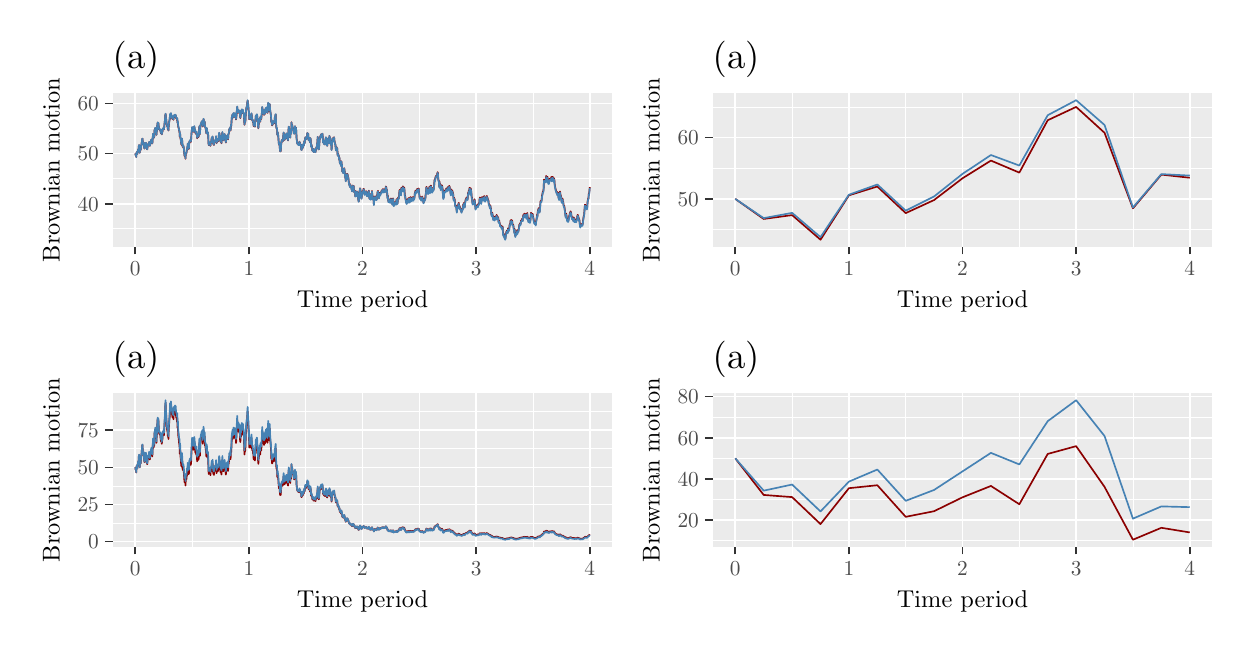
\begin{tikzpicture}[x=1pt,y=1pt]
\definecolor{fillColor}{RGB}{255,255,255}
\path[use as bounding box,fill=fillColor,fill opacity=0.00] (0,0) rectangle (433.62,216.81);
\begin{scope}
\path[clip] (  0.00,108.41) rectangle (216.81,216.81);
\definecolor{drawColor}{RGB}{255,255,255}
\definecolor{fillColor}{RGB}{255,255,255}

\path[draw=drawColor,line width= 0.6pt,line join=round,line cap=round,fill=fillColor] (  0.00,108.41) rectangle (216.81,216.81);
\end{scope}
\begin{scope}
\path[clip] ( 30.68,137.66) rectangle (211.31,193.12);
\definecolor{fillColor}{gray}{0.92}

\path[fill=fillColor] ( 30.68,137.66) rectangle (211.31,193.12);
\definecolor{drawColor}{RGB}{255,255,255}

\path[draw=drawColor,line width= 0.3pt,line join=round] ( 30.68,144.11) --
	(211.31,144.11);

\path[draw=drawColor,line width= 0.3pt,line join=round] ( 30.68,162.24) --
	(211.31,162.24);

\path[draw=drawColor,line width= 0.3pt,line join=round] ( 30.68,180.37) --
	(211.31,180.37);

\path[draw=drawColor,line width= 0.3pt,line join=round] ( 59.42,137.66) --
	( 59.42,193.12);

\path[draw=drawColor,line width= 0.3pt,line join=round] (100.47,137.66) --
	(100.47,193.12);

\path[draw=drawColor,line width= 0.3pt,line join=round] (141.52,137.66) --
	(141.52,193.12);

\path[draw=drawColor,line width= 0.3pt,line join=round] (182.57,137.66) --
	(182.57,193.12);

\path[draw=drawColor,line width= 0.6pt,line join=round] ( 30.68,153.17) --
	(211.31,153.17);

\path[draw=drawColor,line width= 0.6pt,line join=round] ( 30.68,171.30) --
	(211.31,171.30);

\path[draw=drawColor,line width= 0.6pt,line join=round] ( 30.68,189.44) --
	(211.31,189.44);

\path[draw=drawColor,line width= 0.6pt,line join=round] ( 38.89,137.66) --
	( 38.89,193.12);

\path[draw=drawColor,line width= 0.6pt,line join=round] ( 79.94,137.66) --
	( 79.94,193.12);

\path[draw=drawColor,line width= 0.6pt,line join=round] (121.00,137.66) --
	(121.00,193.12);

\path[draw=drawColor,line width= 0.6pt,line join=round] (162.05,137.66) --
	(162.05,193.12);

\path[draw=drawColor,line width= 0.6pt,line join=round] (203.10,137.66) --
	(203.10,193.12);
\definecolor{drawColor}{RGB}{139,0,0}

\path[draw=drawColor,line width= 0.6pt,line join=round] ( 38.89,171.30) --
	( 39.01,170.70) --
	( 39.12,170.87) --
	( 39.23,170.08) --
	( 39.35,171.59) --
	( 39.46,171.90) --
	( 39.58,171.11) --
	( 39.69,171.57) --
	( 39.80,172.27) --
	( 39.92,172.83) --
	( 40.03,172.53) --
	( 40.15,174.00) --
	( 40.26,174.38) --
	( 40.37,173.76) --
	( 40.49,171.60) --
	( 40.60,172.68) --
	( 40.72,172.64) --
	( 40.83,172.62) --
	( 40.94,173.53) --
	( 41.06,174.33) --
	( 41.17,174.91) --
	( 41.29,175.83) --
	( 41.40,176.61) --
	( 41.51,176.68) --
	( 41.63,174.68) --
	( 41.74,175.29) --
	( 41.86,175.23) --
	( 41.97,175.07) --
	( 42.08,173.61) --
	( 42.20,173.14) --
	( 42.31,173.54) --
	( 42.43,174.88) --
	( 42.54,174.77) --
	( 42.65,175.15) --
	( 42.77,175.09) --
	( 42.88,173.73) --
	( 43.00,173.32) --
	( 43.11,172.93) --
	( 43.22,172.86) --
	( 43.34,173.93) --
	( 43.45,174.68) --
	( 43.57,174.51) --
	( 43.68,174.26) --
	( 43.79,174.94) --
	( 43.91,175.49) --
	( 44.02,174.80) --
	( 44.14,174.10) --
	( 44.25,174.45) --
	( 44.36,175.21) --
	( 44.48,175.09) --
	( 44.59,175.97) --
	( 44.71,176.36) --
	( 44.82,175.74) --
	( 44.94,176.08) --
	( 45.05,174.95) --
	( 45.16,176.38) --
	( 45.28,178.39) --
	( 45.39,178.01) --
	( 45.51,176.94) --
	( 45.62,177.51) --
	( 45.73,177.37) --
	( 45.85,179.84) --
	( 45.96,179.79) --
	( 46.08,180.51) --
	( 46.19,180.54) --
	( 46.30,179.75) --
	( 46.42,179.94) --
	( 46.53,178.07) --
	( 46.65,179.58) --
	( 46.76,179.73) --
	( 46.87,182.02) --
	( 46.99,182.53) --
	( 47.10,181.76) --
	( 47.22,182.41) --
	( 47.33,181.40) --
	( 47.44,180.08) --
	( 47.56,180.38) --
	( 47.67,179.91) --
	( 47.79,179.90) --
	( 47.90,179.97) --
	( 48.01,179.35) --
	( 48.13,178.76) --
	( 48.24,178.61) --
	( 48.36,179.83) --
	( 48.47,178.25) --
	( 48.58,178.85) --
	( 48.70,179.19) --
	( 48.81,180.30) --
	( 48.93,179.97) --
	( 49.04,180.36) --
	( 49.15,180.63) --
	( 49.27,180.06) --
	( 49.38,181.32) --
	( 49.50,182.56) --
	( 49.61,183.31) --
	( 49.72,185.03) --
	( 49.84,185.64) --
	( 49.95,184.23) --
	( 50.07,183.60) --
	( 50.18,182.28) --
	( 50.29,181.77) --
	( 50.41,181.10) --
	( 50.52,181.14) --
	( 50.64,180.18) --
	( 50.75,180.34) --
	( 50.86,179.64) --
	( 50.98,181.50) --
	( 51.09,182.26) --
	( 51.21,183.23) --
	( 51.32,183.64) --
	( 51.44,185.48) --
	( 51.55,184.78) --
	( 51.66,184.26) --
	( 51.78,185.83) --
	( 51.89,185.11) --
	( 52.01,184.88) --
	( 52.12,184.44) --
	( 52.23,184.08) --
	( 52.35,183.77) --
	( 52.46,184.31) --
	( 52.58,184.11) --
	( 52.69,183.55) --
	( 52.80,185.01) --
	( 52.92,184.77) --
	( 53.03,184.57) --
	( 53.15,184.45) --
	( 53.26,185.23) --
	( 53.37,185.14) --
	( 53.49,185.10) --
	( 53.60,184.34) --
	( 53.72,183.98) --
	( 53.83,184.04) --
	( 53.94,183.40) --
	( 54.06,183.97) --
	( 54.17,182.32) --
	( 54.29,182.65) --
	( 54.40,181.00) --
	( 54.51,180.68) --
	( 54.63,180.12) --
	( 54.74,179.43) --
	( 54.86,179.37) --
	( 54.97,177.39) --
	( 55.08,178.59) --
	( 55.20,176.88) --
	( 55.31,176.41) --
	( 55.43,175.28) --
	( 55.54,174.53) --
	( 55.65,176.61) --
	( 55.77,176.63) --
	( 55.88,175.33) --
	( 56.00,173.70) --
	( 56.11,174.14) --
	( 56.22,174.11) --
	( 56.34,173.80) --
	( 56.45,172.88) --
	( 56.57,171.44) --
	( 56.68,170.41) --
	( 56.79,171.36) --
	( 56.91,170.76) --
	( 57.02,169.45) --
	( 57.14,171.21) --
	( 57.25,171.62) --
	( 57.36,171.38) --
	( 57.48,172.40) --
	( 57.59,173.25) --
	( 57.71,172.64) --
	( 57.82,174.80) --
	( 57.93,174.55) --
	( 58.05,173.14) --
	( 58.16,173.00) --
	( 58.28,173.19) --
	( 58.39,175.47) --
	( 58.51,175.57) --
	( 58.62,176.02) --
	( 58.73,175.94) --
	( 58.85,175.60) --
	( 58.96,175.56) --
	( 59.08,176.34) --
	( 59.19,178.45) --
	( 59.30,179.51) --
	( 59.42,180.77) --
	( 59.53,179.48) --
	( 59.65,180.50) --
	( 59.76,180.73) --
	( 59.87,179.19) --
	( 59.99,179.72) --
	( 60.10,179.55) --
	( 60.22,181.09) --
	( 60.33,180.27) --
	( 60.44,179.82) --
	( 60.56,178.85) --
	( 60.67,178.66) --
	( 60.79,179.07) --
	( 60.90,178.31) --
	( 61.01,179.16) --
	( 61.13,177.91) --
	( 61.24,176.84) --
	( 61.36,178.30) --
	( 61.47,177.26) --
	( 61.58,177.67) --
	( 61.70,177.28) --
	( 61.81,177.69) --
	( 61.93,179.43) --
	( 62.04,181.09) --
	( 62.15,180.73) --
	( 62.27,178.35) --
	( 62.38,180.95) --
	( 62.50,181.65) --
	( 62.61,182.22) --
	( 62.72,182.20) --
	( 62.84,182.74) --
	( 62.95,182.56) --
	( 63.07,183.01) --
	( 63.18,182.57) --
	( 63.29,181.10) --
	( 63.41,182.15) --
	( 63.52,183.78) --
	( 63.64,183.44) --
	( 63.75,182.09) --
	( 63.86,182.77) --
	( 63.98,182.72) --
	( 64.09,180.86) --
	( 64.21,180.86) --
	( 64.32,180.19) --
	( 64.43,179.83) --
	( 64.55,178.62) --
	( 64.66,180.50) --
	( 64.78,180.14) --
	( 64.89,178.47) --
	( 65.00,178.67) --
	( 65.12,178.93) --
	( 65.23,177.91) --
	( 65.35,174.99) --
	( 65.46,174.35) --
	( 65.58,174.91) --
	( 65.69,174.84) --
	( 65.80,174.74) --
	( 65.92,175.29) --
	( 66.03,174.11) --
	( 66.15,175.19) --
	( 66.26,175.18) --
	( 66.37,175.89) --
	( 66.49,176.92) --
	( 66.60,177.15) --
	( 66.72,176.25) --
	( 66.83,177.42) --
	( 66.94,175.40) --
	( 67.06,174.85) --
	( 67.17,174.59) --
	( 67.29,174.42) --
	( 67.40,175.43) --
	( 67.51,175.56) --
	( 67.63,175.97) --
	( 67.74,175.89) --
	( 67.86,175.64) --
	( 67.97,176.33) --
	( 68.08,177.49) --
	( 68.20,175.06) --
	( 68.31,175.63) --
	( 68.43,176.00) --
	( 68.54,175.57) --
	( 68.65,176.52) --
	( 68.77,176.12) --
	( 68.88,175.83) --
	( 69.00,176.69) --
	( 69.11,178.44) --
	( 69.22,178.71) --
	( 69.34,178.27) --
	( 69.45,177.05) --
	( 69.57,176.71) --
	( 69.68,175.76) --
	( 69.79,175.49) --
	( 69.91,175.88) --
	( 70.02,175.03) --
	( 70.14,177.69) --
	( 70.25,177.85) --
	( 70.36,179.01) --
	( 70.48,176.66) --
	( 70.59,177.40) --
	( 70.71,176.07) --
	( 70.82,176.99) --
	( 70.93,177.39) --
	( 71.05,176.97) --
	( 71.16,178.32) --
	( 71.28,177.59) --
	( 71.39,177.00) --
	( 71.50,175.98) --
	( 71.62,175.31) --
	( 71.73,176.25) --
	( 71.85,176.68) --
	( 71.96,177.70) --
	( 72.08,177.29) --
	( 72.19,177.67) --
	( 72.30,177.92) --
	( 72.42,176.46) --
	( 72.53,178.27) --
	( 72.65,178.40) --
	( 72.76,179.19) --
	( 72.87,180.18) --
	( 72.99,180.12) --
	( 73.10,179.80) --
	( 73.22,180.73) --
	( 73.33,179.62) --
	( 73.44,181.70) --
	( 73.56,181.28) --
	( 73.67,183.05) --
	( 73.79,184.69) --
	( 73.90,184.77) --
	( 74.01,185.39) --
	( 74.13,184.26) --
	( 74.24,184.61) --
	( 74.36,185.75) --
	( 74.47,185.86) --
	( 74.58,185.35) --
	( 74.70,184.62) --
	( 74.81,184.58) --
	( 74.93,185.75) --
	( 75.04,185.21) --
	( 75.15,185.07) --
	( 75.27,183.65) --
	( 75.38,184.18) --
	( 75.50,185.61) --
	( 75.61,187.27) --
	( 75.72,188.19) --
	( 75.84,186.08) --
	( 75.95,186.62) --
	( 76.07,187.12) --
	( 76.18,186.72) --
	( 76.29,186.90) --
	( 76.41,185.93) --
	( 76.52,186.68) --
	( 76.64,186.31) --
	( 76.75,184.57) --
	( 76.86,184.17) --
	( 76.98,185.66) --
	( 77.09,185.29) --
	( 77.21,186.09) --
	( 77.32,187.14) --
	( 77.43,187.14) --
	( 77.55,186.74) --
	( 77.66,186.14) --
	( 77.78,186.96) --
	( 77.89,185.77) --
	( 78.00,186.04) --
	( 78.12,185.71) --
	( 78.23,183.23) --
	( 78.35,181.71) --
	( 78.46,182.69) --
	( 78.57,182.48) --
	( 78.69,183.34) --
	( 78.80,185.39) --
	( 78.92,187.03) --
	( 79.03,187.78) --
	( 79.15,188.21) --
	( 79.26,187.98) --
	( 79.37,189.78) --
	( 79.49,190.46) --
	( 79.60,189.10) --
	( 79.72,188.92) --
	( 79.83,186.75) --
	( 79.94,186.52) --
	( 80.06,183.66) --
	( 80.17,185.09) --
	( 80.29,184.39) --
	( 80.40,183.91) --
	( 80.51,183.72) --
	( 80.63,184.39) --
	( 80.74,185.12) --
	( 80.86,185.75) --
	( 80.97,185.11) --
	( 81.08,183.61) --
	( 81.20,183.19) --
	( 81.31,183.48) --
	( 81.43,182.59) --
	( 81.54,182.51) --
	( 81.65,181.26) --
	( 81.77,181.24) --
	( 81.88,181.37) --
	( 82.00,181.21) --
	( 82.11,181.03) --
	( 82.22,182.91) --
	( 82.34,183.73) --
	( 82.45,184.94) --
	( 82.57,183.92) --
	( 82.68,184.10) --
	( 82.79,185.36) --
	( 82.91,185.29) --
	( 83.02,182.96) --
	( 83.14,183.33) --
	( 83.25,181.28) --
	( 83.36,180.42) --
	( 83.48,181.82) --
	( 83.59,182.47) --
	( 83.71,183.64) --
	( 83.82,183.97) --
	( 83.93,183.84) --
	( 84.05,182.84) --
	( 84.16,184.56) --
	( 84.28,184.61) --
	( 84.39,183.82) --
	( 84.50,184.76) --
	( 84.62,185.94) --
	( 84.73,188.06) --
	( 84.85,187.37) --
	( 84.96,186.93) --
	( 85.07,186.45) --
	( 85.19,186.03) --
	( 85.30,185.62) --
	( 85.42,185.29) --
	( 85.53,186.88) --
	( 85.65,186.10) --
	( 85.76,185.66) --
	( 85.87,186.38) --
	( 85.99,187.64) --
	( 86.10,186.76) --
	( 86.22,186.19) --
	( 86.33,186.77) --
	( 86.44,187.91) --
	( 86.56,187.62) --
	( 86.67,186.01) --
	( 86.79,187.92) --
	( 86.90,189.55) --
	( 87.01,188.73) --
	( 87.13,188.65) --
	( 87.24,186.66) --
	( 87.36,187.29) --
	( 87.47,189.12) --
	( 87.58,187.25) --
	( 87.70,186.38) --
	( 87.81,185.66) --
	( 87.93,184.90) --
	( 88.04,182.68) --
	( 88.15,183.22) --
	( 88.27,181.57) --
	( 88.38,181.54) --
	( 88.50,182.16) --
	( 88.61,181.95) --
	( 88.72,182.90) --
	( 88.84,182.87) --
	( 88.95,182.16) --
	( 89.07,182.85) --
	( 89.18,182.38) --
	( 89.29,184.29) --
	( 89.41,184.27) --
	( 89.52,185.20) --
	( 89.64,185.42) --
	( 89.75,182.14) --
	( 89.86,180.69) --
	( 89.98,180.23) --
	( 90.09,180.48) --
	( 90.21,178.04) --
	( 90.32,179.02) --
	( 90.43,178.39) --
	( 90.55,177.62) --
	( 90.66,176.03) --
	( 90.78,174.58) --
	( 90.89,174.63) --
	( 91.00,175.13) --
	( 91.12,173.06) --
	( 91.23,172.08) --
	( 91.35,172.59) --
	( 91.46,172.15) --
	( 91.57,174.26) --
	( 91.69,175.49) --
	( 91.80,176.08) --
	( 91.92,176.08) --
	( 92.03,176.36) --
	( 92.14,175.64) --
	( 92.26,176.27) --
	( 92.37,177.76) --
	( 92.49,178.87) --
	( 92.60,178.03) --
	( 92.72,176.38) --
	( 92.83,176.26) --
	( 92.94,176.70) --
	( 93.06,178.07) --
	( 93.17,176.72) --
	( 93.29,177.09) --
	( 93.40,177.32) --
	( 93.51,178.54) --
	( 93.63,178.51) --
	( 93.74,178.13) --
	( 93.86,176.96) --
	( 93.97,176.43) --
	( 94.08,176.06) --
	( 94.20,178.44) --
	( 94.31,180.99) --
	( 94.43,180.81) --
	( 94.54,179.71) --
	( 94.65,177.67) --
	( 94.77,178.19) --
	( 94.88,177.07) --
	( 95.00,179.41) --
	( 95.11,178.49) --
	( 95.22,178.60) --
	( 95.34,182.61) --
	( 95.45,181.42) --
	( 95.57,181.74) --
	( 95.68,180.56) --
	( 95.79,180.92) --
	( 95.91,180.00) --
	( 96.02,180.07) --
	( 96.14,179.76) --
	( 96.25,178.52) --
	( 96.36,178.53) --
	( 96.48,179.55) --
	( 96.59,181.22) --
	( 96.71,179.77) --
	( 96.82,179.51) --
	( 96.93,180.72) --
	( 97.05,179.54) --
	( 97.16,176.94) --
	( 97.28,175.99) --
	( 97.39,175.01) --
	( 97.50,175.05) --
	( 97.62,174.65) --
	( 97.73,174.87) --
	( 97.85,174.45) --
	( 97.96,174.81) --
	( 98.07,174.45) --
	( 98.19,175.63) --
	( 98.30,174.89) --
	( 98.42,175.17) --
	( 98.53,174.29) --
	( 98.64,174.49) --
	( 98.76,174.43) --
	( 98.87,172.78) --
	( 98.99,172.63) --
	( 99.10,173.78) --
	( 99.22,174.45) --
	( 99.33,174.58) --
	( 99.44,173.40) --
	( 99.56,174.55) --
	( 99.67,174.62) --
	( 99.79,174.17) --
	( 99.90,175.80) --
	(100.01,175.02) --
	(100.13,175.32) --
	(100.24,176.60) --
	(100.36,177.21) --
	(100.47,176.89) --
	(100.58,176.46) --
	(100.70,176.82) --
	(100.81,177.33) --
	(100.93,177.35) --
	(101.04,178.70) --
	(101.15,178.62) --
	(101.27,177.90) --
	(101.38,178.44) --
	(101.50,176.19) --
	(101.61,176.58) --
	(101.72,177.08) --
	(101.84,176.85) --
	(101.95,175.72) --
	(102.07,175.32) --
	(102.18,176.87) --
	(102.29,176.11) --
	(102.41,173.79) --
	(102.52,174.59) --
	(102.64,174.09) --
	(102.75,173.58) --
	(102.86,172.39) --
	(102.98,172.37) --
	(103.09,173.04) --
	(103.21,172.47) --
	(103.32,171.87) --
	(103.43,172.93) --
	(103.55,172.68) --
	(103.66,172.52) --
	(103.78,171.92) --
	(103.89,172.78) --
	(104.00,171.82) --
	(104.12,172.63) --
	(104.23,173.41) --
	(104.35,172.95) --
	(104.46,173.77) --
	(104.57,174.74) --
	(104.69,175.31) --
	(104.80,177.34) --
	(104.92,175.36) --
	(105.03,174.20) --
	(105.14,172.85) --
	(105.26,173.00) --
	(105.37,174.55) --
	(105.49,176.22) --
	(105.60,176.71) --
	(105.71,177.60) --
	(105.83,177.45) --
	(105.94,177.92) --
	(106.06,178.30) --
	(106.17,177.52) --
	(106.29,177.21) --
	(106.40,177.07) --
	(106.51,178.49) --
	(106.63,177.42) --
	(106.74,175.28) --
	(106.86,176.05) --
	(106.97,175.23) --
	(107.08,174.79) --
	(107.20,175.68) --
	(107.31,174.92) --
	(107.43,174.57) --
	(107.54,176.07) --
	(107.65,176.60) --
	(107.77,177.14) --
	(107.88,177.00) --
	(108.00,175.84) --
	(108.11,174.35) --
	(108.22,174.12) --
	(108.34,176.11) --
	(108.45,176.33) --
	(108.57,176.49) --
	(108.68,176.82) --
	(108.79,176.43) --
	(108.91,175.02) --
	(109.02,177.71) --
	(109.14,177.27) --
	(109.25,176.97) --
	(109.36,175.16) --
	(109.48,174.91) --
	(109.59,174.65) --
	(109.71,174.40) --
	(109.82,172.64) --
	(109.93,174.38) --
	(110.05,176.14) --
	(110.16,176.83) --
	(110.28,175.71) --
	(110.39,176.43) --
	(110.50,176.17) --
	(110.62,175.85) --
	(110.73,177.22) --
	(110.85,175.97) --
	(110.96,175.45) --
	(111.07,174.72) --
	(111.19,174.74) --
	(111.30,173.18) --
	(111.42,172.49) --
	(111.53,173.19) --
	(111.64,173.64) --
	(111.76,172.68) --
	(111.87,173.22) --
	(111.99,170.87) --
	(112.10,170.54) --
	(112.21,171.22) --
	(112.33,170.58) --
	(112.44,170.54) --
	(112.56,169.04) --
	(112.67,169.83) --
	(112.79,168.10) --
	(112.90,167.80) --
	(113.01,167.56) --
	(113.13,167.61) --
	(113.24,166.86) --
	(113.36,168.53) --
	(113.47,167.21) --
	(113.58,167.44) --
	(113.70,164.78) --
	(113.81,164.78) --
	(113.93,165.23) --
	(114.04,164.26) --
	(114.15,164.88) --
	(114.27,165.17) --
	(114.38,166.04) --
	(114.50,165.28) --
	(114.61,164.42) --
	(114.72,162.86) --
	(114.84,162.58) --
	(114.95,161.43) --
	(115.07,162.01) --
	(115.18,162.07) --
	(115.29,163.96) --
	(115.41,162.95) --
	(115.52,163.97) --
	(115.64,163.51) --
	(115.75,162.24) --
	(115.86,162.73) --
	(115.98,161.50) --
	(116.09,160.60) --
	(116.21,159.98) --
	(116.32,160.15) --
	(116.43,159.31) --
	(116.55,160.21) --
	(116.66,159.20) --
	(116.78,159.38) --
	(116.89,159.49) --
	(117.00,158.61) --
	(117.12,158.25) --
	(117.23,157.71) --
	(117.35,158.49) --
	(117.46,159.77) --
	(117.57,158.91) --
	(117.69,159.67) --
	(117.80,159.61) --
	(117.92,157.98) --
	(118.03,157.36) --
	(118.14,157.73) --
	(118.26,157.85) --
	(118.37,155.88) --
	(118.49,156.34) --
	(118.60,156.86) --
	(118.71,156.61) --
	(118.83,156.04) --
	(118.94,157.62) --
	(119.06,157.54) --
	(119.17,157.53) --
	(119.28,156.62) --
	(119.40,155.54) --
	(119.51,154.35) --
	(119.63,154.02) --
	(119.74,155.07) --
	(119.86,156.46) --
	(119.97,157.72) --
	(120.08,158.77) --
	(120.20,158.57) --
	(120.31,157.57) --
	(120.43,157.30) --
	(120.54,155.37) --
	(120.65,155.12) --
	(120.77,156.43) --
	(120.88,156.53) --
	(121.00,157.41) --
	(121.11,157.80) --
	(121.22,157.17) --
	(121.34,158.58) --
	(121.45,158.51) --
	(121.57,157.71) --
	(121.68,157.76) --
	(121.79,156.54) --
	(121.91,157.23) --
	(122.02,157.63) --
	(122.14,157.34) --
	(122.25,156.94) --
	(122.36,157.69) --
	(122.48,156.83) --
	(122.59,156.04) --
	(122.71,156.37) --
	(122.82,156.01) --
	(122.93,156.74) --
	(123.05,156.58) --
	(123.16,157.54) --
	(123.28,157.94) --
	(123.39,156.12) --
	(123.50,155.06) --
	(123.62,156.07) --
	(123.73,156.62) --
	(123.85,155.85) --
	(123.96,154.78) --
	(124.07,155.59) --
	(124.19,154.95) --
	(124.30,156.37) --
	(124.42,157.79) --
	(124.53,156.61) --
	(124.64,155.93) --
	(124.76,154.94) --
	(124.87,155.46) --
	(124.99,154.45) --
	(125.10,152.88) --
	(125.21,154.43) --
	(125.33,155.21) --
	(125.44,155.85) --
	(125.56,155.33) --
	(125.67,155.31) --
	(125.78,155.80) --
	(125.90,154.79) --
	(126.01,154.68) --
	(126.13,154.82) --
	(126.24,156.15) --
	(126.36,156.66) --
	(126.47,157.69) --
	(126.58,157.80) --
	(126.70,156.89) --
	(126.81,156.62) --
	(126.93,155.29) --
	(127.04,156.02) --
	(127.15,157.15) --
	(127.27,157.10) --
	(127.38,156.31) --
	(127.50,157.17) --
	(127.61,157.28) --
	(127.72,156.97) --
	(127.84,157.87) --
	(127.95,157.25) --
	(128.07,158.18) --
	(128.18,157.49) --
	(128.29,157.80) --
	(128.41,158.53) --
	(128.52,157.43) --
	(128.64,157.75) --
	(128.75,157.66) --
	(128.86,158.20) --
	(128.98,157.56) --
	(129.09,157.48) --
	(129.21,158.61) --
	(129.32,158.74) --
	(129.43,159.42) --
	(129.55,159.23) --
	(129.66,158.38) --
	(129.78,158.36) --
	(129.89,157.36) --
	(130.00,155.29) --
	(130.12,156.21) --
	(130.23,155.34) --
	(130.35,153.92) --
	(130.46,154.68) --
	(130.57,154.67) --
	(130.69,154.20) --
	(130.80,154.06) --
	(130.92,153.73) --
	(131.03,154.49) --
	(131.14,155.06) --
	(131.26,153.71) --
	(131.37,153.98) --
	(131.49,154.54) --
	(131.60,155.06) --
	(131.71,153.18) --
	(131.83,152.99) --
	(131.94,154.51) --
	(132.06,155.13) --
	(132.17,153.80) --
	(132.28,152.52) --
	(132.40,152.89) --
	(132.51,152.76) --
	(132.63,153.49) --
	(132.74,153.71) --
	(132.85,153.77) --
	(132.97,153.90) --
	(133.08,154.03) --
	(133.20,153.05) --
	(133.31,154.86) --
	(133.43,153.76) --
	(133.54,153.74) --
	(133.65,153.32) --
	(133.77,154.71) --
	(133.88,155.50) --
	(134.00,155.05) --
	(134.11,155.21) --
	(134.22,156.13) --
	(134.34,157.92) --
	(134.45,158.16) --
	(134.57,157.31) --
	(134.68,156.52) --
	(134.79,158.13) --
	(134.91,156.46) --
	(135.02,158.93) --
	(135.14,158.72) --
	(135.25,158.34) --
	(135.36,158.46) --
	(135.48,159.23) --
	(135.59,159.47) --
	(135.71,157.86) --
	(135.82,158.15) --
	(135.93,158.51) --
	(136.05,159.05) --
	(136.16,158.20) --
	(136.28,156.28) --
	(136.39,156.02) --
	(136.50,155.27) --
	(136.62,154.66) --
	(136.73,153.92) --
	(136.85,153.61) --
	(136.96,153.36) --
	(137.07,153.97) --
	(137.19,154.73) --
	(137.30,154.11) --
	(137.42,153.87) --
	(137.53,154.14) --
	(137.64,155.23) --
	(137.76,155.18) --
	(137.87,153.86) --
	(137.99,154.03) --
	(138.10,153.94) --
	(138.21,155.31) --
	(138.33,155.58) --
	(138.44,155.09) --
	(138.56,154.74) --
	(138.67,154.34) --
	(138.78,154.48) --
	(138.90,154.61) --
	(139.01,155.33) --
	(139.13,155.58) --
	(139.24,155.28) --
	(139.35,154.54) --
	(139.47,155.03) --
	(139.58,154.98) --
	(139.70,155.12) --
	(139.81,155.99) --
	(139.93,157.39) --
	(140.04,156.62) --
	(140.15,157.94) --
	(140.27,157.23) --
	(140.38,157.44) --
	(140.50,157.62) --
	(140.61,157.39) --
	(140.72,158.52) --
	(140.84,157.98) --
	(140.95,158.51) --
	(141.07,158.50) --
	(141.18,157.73) --
	(141.29,158.72) --
	(141.41,157.02) --
	(141.52,156.59) --
	(141.64,155.36) --
	(141.75,155.51) --
	(141.86,155.72) --
	(141.98,154.83) --
	(142.09,155.34) --
	(142.21,154.53) --
	(142.32,155.04) --
	(142.43,155.22) --
	(142.55,155.78) --
	(142.66,155.04) --
	(142.78,155.11) --
	(142.89,154.74) --
	(143.00,153.60) --
	(143.12,153.71) --
	(143.23,155.09) --
	(143.35,154.58) --
	(143.46,154.42) --
	(143.57,154.95) --
	(143.69,154.98) --
	(143.80,156.51) --
	(143.92,157.10) --
	(144.03,158.99) --
	(144.14,159.27) --
	(144.26,158.33) --
	(144.37,158.67) --
	(144.49,157.91) --
	(144.60,157.09) --
	(144.71,156.94) --
	(144.83,157.69) --
	(144.94,157.96) --
	(145.06,158.62) --
	(145.17,159.38) --
	(145.28,159.23) --
	(145.40,157.26) --
	(145.51,157.90) --
	(145.63,159.68) --
	(145.74,159.73) --
	(145.85,158.60) --
	(145.97,158.30) --
	(146.08,157.53) --
	(146.20,157.49) --
	(146.31,158.04) --
	(146.42,158.74) --
	(146.54,158.93) --
	(146.65,158.16) --
	(146.77,158.82) --
	(146.88,159.94) --
	(147.00,161.84) --
	(147.11,161.41) --
	(147.22,161.81) --
	(147.34,162.84) --
	(147.45,162.73) --
	(147.57,163.18) --
	(147.68,163.36) --
	(147.79,163.24) --
	(147.91,163.39) --
	(148.02,164.23) --
	(148.14,164.58) --
	(148.25,164.17) --
	(148.36,162.21) --
	(148.48,161.53) --
	(148.59,161.51) --
	(148.71,159.39) --
	(148.82,161.24) --
	(148.93,159.98) --
	(149.05,159.01) --
	(149.16,160.22) --
	(149.28,158.40) --
	(149.39,159.00) --
	(149.50,158.72) --
	(149.62,159.09) --
	(149.73,159.81) --
	(149.85,159.01) --
	(149.96,158.43) --
	(150.07,156.00) --
	(150.19,155.24) --
	(150.30,155.54) --
	(150.42,155.93) --
	(150.53,157.55) --
	(150.64,157.60) --
	(150.76,157.97) --
	(150.87,158.03) --
	(150.99,157.63) --
	(151.10,158.24) --
	(151.21,158.61) --
	(151.33,158.71) --
	(151.44,158.04) --
	(151.56,158.00) --
	(151.67,158.64) --
	(151.78,159.19) --
	(151.90,158.79) --
	(152.01,158.24) --
	(152.13,158.65) --
	(152.24,159.52) --
	(152.35,159.61) --
	(152.47,159.35) --
	(152.58,158.62) --
	(152.70,158.27) --
	(152.81,157.06) --
	(152.92,156.50) --
	(153.04,157.41) --
	(153.15,158.31) --
	(153.27,157.59) --
	(153.38,157.76) --
	(153.50,157.81) --
	(153.61,156.47) --
	(153.72,157.11) --
	(153.84,155.58) --
	(153.95,154.60) --
	(154.07,155.38) --
	(154.18,154.95) --
	(154.29,154.78) --
	(154.41,153.52) --
	(154.52,152.41) --
	(154.64,152.67) --
	(154.75,152.53) --
	(154.86,152.08) --
	(154.98,151.08) --
	(155.09,150.26) --
	(155.21,151.77) --
	(155.32,151.52) --
	(155.43,152.10) --
	(155.55,152.69) --
	(155.66,153.27) --
	(155.78,153.49) --
	(155.89,152.53) --
	(156.00,151.77) --
	(156.12,152.33) --
	(156.23,151.34) --
	(156.35,151.73) --
	(156.46,151.33) --
	(156.57,151.03) --
	(156.69,150.44) --
	(156.80,150.27) --
	(156.92,150.91) --
	(157.03,151.24) --
	(157.14,151.07) --
	(157.26,151.71) --
	(157.37,152.96) --
	(157.49,152.95) --
	(157.60,153.31) --
	(157.71,153.52) --
	(157.83,152.76) --
	(157.94,152.06) --
	(158.06,153.51) --
	(158.17,154.19) --
	(158.28,154.76) --
	(158.40,154.88) --
	(158.51,155.25) --
	(158.63,155.37) --
	(158.74,155.40) --
	(158.85,155.57) --
	(158.97,154.77) --
	(159.08,156.67) --
	(159.20,157.31) --
	(159.31,157.10) --
	(159.42,158.08) --
	(159.54,157.57) --
	(159.65,158.96) --
	(159.77,158.63) --
	(159.88,156.74) --
	(159.99,157.84) --
	(160.11,158.76) --
	(160.22,158.12) --
	(160.34,156.98) --
	(160.45,155.51) --
	(160.57,155.29) --
	(160.68,153.86) --
	(160.79,153.23) --
	(160.91,153.35) --
	(161.02,154.01) --
	(161.14,153.37) --
	(161.25,153.27) --
	(161.36,153.46) --
	(161.48,154.79) --
	(161.59,154.04) --
	(161.71,152.81) --
	(161.82,151.41) --
	(161.93,151.82) --
	(162.05,151.78) --
	(162.16,152.35) --
	(162.28,152.24) --
	(162.39,152.54) --
	(162.50,152.70) --
	(162.62,152.72) --
	(162.73,152.24) --
	(162.85,153.19) --
	(162.96,152.88) --
	(163.07,153.39) --
	(163.19,153.51) --
	(163.30,154.89) --
	(163.42,155.44) --
	(163.53,155.17) --
	(163.64,155.16) --
	(163.76,155.06) --
	(163.87,153.43) --
	(163.99,154.74) --
	(164.10,155.57) --
	(164.21,154.96) --
	(164.33,155.26) --
	(164.44,155.45) --
	(164.56,154.55) --
	(164.67,155.72) --
	(164.78,155.52) --
	(164.90,155.66) --
	(165.01,155.98) --
	(165.13,155.19) --
	(165.24,154.34) --
	(165.35,154.29) --
	(165.47,154.74) --
	(165.58,154.79) --
	(165.70,155.34) --
	(165.81,155.60) --
	(165.92,156.03) --
	(166.04,154.92) --
	(166.15,155.45) --
	(166.27,154.82) --
	(166.38,154.46) --
	(166.49,154.37) --
	(166.61,153.10) --
	(166.72,153.02) --
	(166.84,152.68) --
	(166.95,152.13) --
	(167.06,151.71) --
	(167.18,152.64) --
	(167.29,151.69) --
	(167.41,151.53) --
	(167.52,149.70) --
	(167.64,149.21) --
	(167.75,148.84) --
	(167.86,149.96) --
	(167.98,149.25) --
	(168.09,148.62) --
	(168.21,147.62) --
	(168.32,147.75) --
	(168.43,148.56) --
	(168.55,147.71) --
	(168.66,147.40) --
	(168.78,148.37) --
	(168.89,147.88) --
	(169.00,148.36) --
	(169.12,148.64) --
	(169.23,147.70) --
	(169.35,148.57) --
	(169.46,149.13) --
	(169.57,148.78) --
	(169.69,148.13) --
	(169.80,147.85) --
	(169.92,148.42) --
	(170.03,148.02) --
	(170.14,146.70) --
	(170.26,146.59) --
	(170.37,147.13) --
	(170.49,146.32) --
	(170.60,146.15) --
	(170.71,145.31) --
	(170.83,145.38) --
	(170.94,145.29) --
	(171.06,145.26) --
	(171.17,144.84) --
	(171.28,144.35) --
	(171.40,144.94) --
	(171.51,145.01) --
	(171.63,144.88) --
	(171.74,142.73) --
	(171.85,141.90) --
	(171.97,142.39) --
	(172.08,142.12) --
	(172.20,141.34) --
	(172.31,141.06) --
	(172.42,140.82) --
	(172.54,140.50) --
	(172.65,140.81) --
	(172.77,141.78) --
	(172.88,142.41) --
	(172.99,143.23) --
	(173.11,143.01) --
	(173.22,143.56) --
	(173.34,142.91) --
	(173.45,142.81) --
	(173.56,144.26) --
	(173.68,144.25) --
	(173.79,144.04) --
	(173.91,143.65) --
	(174.02,144.16) --
	(174.14,145.58) --
	(174.25,145.86) --
	(174.36,145.68) --
	(174.48,147.11) --
	(174.59,146.56) --
	(174.71,147.35) --
	(174.82,147.05) --
	(174.93,146.33) --
	(175.05,147.18) --
	(175.16,145.93) --
	(175.28,145.71) --
	(175.39,145.72) --
	(175.50,145.41) --
	(175.62,144.30) --
	(175.73,143.87) --
	(175.85,142.83) --
	(175.96,144.10) --
	(176.07,142.87) --
	(176.19,141.50) --
	(176.30,141.95) --
	(176.42,142.53) --
	(176.53,142.40) --
	(176.64,142.26) --
	(176.76,142.73) --
	(176.87,143.65) --
	(176.99,142.60) --
	(177.10,143.46) --
	(177.21,143.58) --
	(177.33,143.35) --
	(177.44,144.19) --
	(177.56,144.82) --
	(177.67,145.69) --
	(177.78,145.48) --
	(177.90,146.01) --
	(178.01,146.21) --
	(178.13,145.85) --
	(178.24,147.07) --
	(178.35,147.18) --
	(178.47,147.14) --
	(178.58,147.50) --
	(178.70,147.78) --
	(178.81,147.28) --
	(178.92,147.23) --
	(179.04,149.08) --
	(179.15,149.03) --
	(179.27,148.81) --
	(179.38,149.34) --
	(179.49,149.63) --
	(179.61,149.23) --
	(179.72,148.45) --
	(179.84,149.05) --
	(179.95,149.14) --
	(180.06,149.48) --
	(180.18,149.27) --
	(180.29,148.08) --
	(180.41,148.12) --
	(180.52,149.84) --
	(180.63,148.78) --
	(180.75,148.07) --
	(180.86,147.13) --
	(180.98,146.87) --
	(181.09,147.83) --
	(181.21,147.72) --
	(181.32,147.54) --
	(181.43,146.63) --
	(181.55,146.67) --
	(181.66,147.39) --
	(181.78,149.00) --
	(181.89,149.95) --
	(182.00,149.31) --
	(182.12,148.95) --
	(182.23,149.38) --
	(182.35,149.37) --
	(182.46,149.57) --
	(182.57,148.62) --
	(182.69,148.31) --
	(182.80,147.65) --
	(182.92,146.99) --
	(183.03,146.48) --
	(183.14,146.19) --
	(183.26,146.19) --
	(183.37,146.62) --
	(183.49,146.26) --
	(183.60,145.67) --
	(183.71,146.78) --
	(183.83,147.48) --
	(183.94,147.97) --
	(184.06,149.18) --
	(184.17,148.47) --
	(184.28,149.95) --
	(184.40,150.85) --
	(184.51,151.07) --
	(184.63,151.53) --
	(184.74,151.57) --
	(184.85,151.49) --
	(184.97,150.32) --
	(185.08,150.86) --
	(185.20,152.46) --
	(185.31,154.06) --
	(185.42,154.18) --
	(185.54,154.10) --
	(185.65,154.23) --
	(185.77,155.12) --
	(185.88,156.29) --
	(185.99,156.61) --
	(186.11,157.50) --
	(186.22,157.48) --
	(186.34,157.88) --
	(186.45,158.84) --
	(186.56,161.90) --
	(186.68,161.85) --
	(186.79,161.27) --
	(186.91,161.65) --
	(187.02,161.30) --
	(187.13,161.83) --
	(187.25,162.12) --
	(187.36,163.25) --
	(187.48,162.42) --
	(187.59,161.38) --
	(187.71,162.72) --
	(187.82,162.91) --
	(187.93,162.11) --
	(188.05,161.19) --
	(188.16,160.72) --
	(188.28,161.21) --
	(188.39,160.76) --
	(188.50,161.90) --
	(188.62,162.10) --
	(188.73,162.27) --
	(188.85,162.25) --
	(188.96,161.99) --
	(189.07,161.84) --
	(189.19,162.83) --
	(189.30,161.68) --
	(189.42,162.61) --
	(189.53,162.30) --
	(189.64,162.93) --
	(189.76,162.87) --
	(189.87,161.71) --
	(189.99,162.00) --
	(190.10,161.45) --
	(190.21,162.41) --
	(190.33,161.70) --
	(190.44,160.18) --
	(190.56,159.46) --
	(190.67,158.99) --
	(190.78,158.30) --
	(190.90,158.10) --
	(191.01,157.61) --
	(191.13,157.28) --
	(191.24,157.54) --
	(191.35,156.60) --
	(191.47,157.20) --
	(191.58,157.20) --
	(191.70,157.16) --
	(191.81,155.53) --
	(191.92,155.29) --
	(192.04,154.85) --
	(192.15,155.51) --
	(192.27,156.62) --
	(192.38,157.60) --
	(192.49,156.70) --
	(192.61,156.06) --
	(192.72,155.99) --
	(192.84,155.15) --
	(192.95,153.89) --
	(193.06,154.50) --
	(193.18,154.55) --
	(193.29,155.03) --
	(193.41,154.09) --
	(193.52,153.82) --
	(193.63,152.92) --
	(193.75,152.28) --
	(193.86,152.45) --
	(193.98,151.83) --
	(194.09,151.09) --
	(194.20,150.12) --
	(194.32,149.08) --
	(194.43,148.45) --
	(194.55,149.68) --
	(194.66,149.20) --
	(194.78,148.39) --
	(194.89,147.39) --
	(195.00,147.28) --
	(195.12,147.00) --
	(195.23,147.18) --
	(195.35,146.98) --
	(195.46,147.58) --
	(195.57,148.09) --
	(195.69,148.84) --
	(195.80,149.01) --
	(195.92,149.81) --
	(196.03,149.75) --
	(196.14,150.43) --
	(196.26,150.31) --
	(196.37,149.81) --
	(196.49,148.92) --
	(196.60,148.41) --
	(196.71,147.88) --
	(196.83,148.28) --
	(196.94,148.24) --
	(197.06,147.79) --
	(197.17,147.15) --
	(197.28,148.22) --
	(197.40,148.05) --
	(197.51,147.16) --
	(197.63,146.86) --
	(197.74,146.92) --
	(197.85,147.50) --
	(197.97,147.43) --
	(198.08,147.51) --
	(198.20,146.78) --
	(198.31,147.33) --
	(198.42,147.40) --
	(198.54,147.91) --
	(198.65,149.02) --
	(198.77,149.14) --
	(198.88,148.93) --
	(198.99,148.38) --
	(199.11,147.97) --
	(199.22,147.32) --
	(199.34,147.57) --
	(199.45,146.54) --
	(199.56,145.34) --
	(199.68,144.88) --
	(199.79,145.62) --
	(199.91,145.70) --
	(200.02,145.35) --
	(200.13,145.81) --
	(200.25,145.56) --
	(200.36,145.48) --
	(200.48,145.53) --
	(200.59,146.27) --
	(200.70,147.17) --
	(200.82,148.07) --
	(200.93,148.77) --
	(201.05,149.00) --
	(201.16,150.36) --
	(201.28,151.88) --
	(201.39,152.88) --
	(201.50,152.71) --
	(201.62,151.92) --
	(201.73,152.06) --
	(201.85,151.64) --
	(201.96,151.84) --
	(202.07,151.42) --
	(202.19,152.11) --
	(202.30,153.78) --
	(202.42,154.52) --
	(202.53,155.09) --
	(202.64,155.12) --
	(202.76,156.85) --
	(202.87,156.78) --
	(202.99,157.89) --
	(203.10,159.18);
\definecolor{drawColor}{RGB}{70,130,180}

\path[draw=drawColor,line width= 0.6pt,line join=round] ( 38.89,171.30) --
	( 39.01,170.71) --
	( 39.12,170.88) --
	( 39.23,170.09) --
	( 39.35,171.59) --
	( 39.46,171.90) --
	( 39.58,171.12) --
	( 39.69,171.58) --
	( 39.80,172.29) --
	( 39.92,172.84) --
	( 40.03,172.55) --
	( 40.15,174.01) --
	( 40.26,174.40) --
	( 40.37,173.78) --
	( 40.49,171.61) --
	( 40.60,172.69) --
	( 40.72,172.64) --
	( 40.83,172.63) --
	( 40.94,173.54) --
	( 41.06,174.35) --
	( 41.17,174.93) --
	( 41.29,175.85) --
	( 41.40,176.63) --
	( 41.51,176.71) --
	( 41.63,174.69) --
	( 41.74,175.31) --
	( 41.86,175.25) --
	( 41.97,175.10) --
	( 42.08,173.63) --
	( 42.20,173.16) --
	( 42.31,173.57) --
	( 42.43,174.90) --
	( 42.54,174.80) --
	( 42.65,175.18) --
	( 42.77,175.13) --
	( 42.88,173.76) --
	( 43.00,173.35) --
	( 43.11,172.97) --
	( 43.22,172.91) --
	( 43.34,173.98) --
	( 43.45,174.73) --
	( 43.57,174.57) --
	( 43.68,174.31) --
	( 43.79,175.00) --
	( 43.91,175.56) --
	( 44.02,174.87) --
	( 44.14,174.16) --
	( 44.25,174.52) --
	( 44.36,175.28) --
	( 44.48,175.17) --
	( 44.59,176.05) --
	( 44.71,176.45) --
	( 44.82,175.83) --
	( 44.94,176.17) --
	( 45.05,175.04) --
	( 45.16,176.46) --
	( 45.28,178.46) --
	( 45.39,178.08) --
	( 45.51,177.01) --
	( 45.62,177.59) --
	( 45.73,177.45) --
	( 45.85,179.90) --
	( 45.96,179.86) --
	( 46.08,180.58) --
	( 46.19,180.61) --
	( 46.30,179.83) --
	( 46.42,180.02) --
	( 46.53,178.13) --
	( 46.65,179.64) --
	( 46.76,179.80) --
	( 46.87,182.07) --
	( 46.99,182.58) --
	( 47.10,181.81) --
	( 47.22,182.46) --
	( 47.33,181.46) --
	( 47.44,180.13) --
	( 47.56,180.44) --
	( 47.67,179.97) --
	( 47.79,179.97) --
	( 47.90,180.05) --
	( 48.01,179.43) --
	( 48.13,178.84) --
	( 48.24,178.70) --
	( 48.36,179.92) --
	( 48.47,178.32) --
	( 48.58,178.94) --
	( 48.70,179.28) --
	( 48.81,180.38) --
	( 48.93,180.06) --
	( 49.04,180.45) --
	( 49.15,180.73) --
	( 49.27,180.16) --
	( 49.38,181.43) --
	( 49.50,182.66) --
	( 49.61,183.41) --
	( 49.72,185.13) --
	( 49.84,185.74) --
	( 49.95,184.33) --
	( 50.07,183.70) --
	( 50.18,182.37) --
	( 50.29,181.87) --
	( 50.41,181.21) --
	( 50.52,181.25) --
	( 50.64,180.29) --
	( 50.75,180.45) --
	( 50.86,179.76) --
	( 50.98,181.61) --
	( 51.09,182.37) --
	( 51.21,183.34) --
	( 51.32,183.76) --
	( 51.44,185.59) --
	( 51.55,184.88) --
	( 51.66,184.38) --
	( 51.78,185.94) --
	( 51.89,185.22) --
	( 52.01,184.99) --
	( 52.12,184.56) --
	( 52.23,184.21) --
	( 52.35,183.91) --
	( 52.46,184.44) --
	( 52.58,184.25) --
	( 52.69,183.70) --
	( 52.80,185.15) --
	( 52.92,184.92) --
	( 53.03,184.72) --
	( 53.15,184.61) --
	( 53.26,185.39) --
	( 53.37,185.31) --
	( 53.49,185.27) --
	( 53.60,184.52) --
	( 53.72,184.16) --
	( 53.83,184.23) --
	( 53.94,183.59) --
	( 54.06,184.16) --
	( 54.17,182.51) --
	( 54.29,182.84) --
	( 54.40,181.19) --
	( 54.51,180.87) --
	( 54.63,180.31) --
	( 54.74,179.63) --
	( 54.86,179.57) --
	( 54.97,177.58) --
	( 55.08,178.78) --
	( 55.20,177.06) --
	( 55.31,176.59) --
	( 55.43,175.46) --
	( 55.54,174.71) --
	( 55.65,176.78) --
	( 55.77,176.79) --
	( 55.88,175.49) --
	( 56.00,173.86) --
	( 56.11,174.30) --
	( 56.22,174.28) --
	( 56.34,173.97) --
	( 56.45,173.05) --
	( 56.57,171.61) --
	( 56.68,170.58) --
	( 56.79,171.52) --
	( 56.91,170.93) --
	( 57.02,169.61) --
	( 57.14,171.36) --
	( 57.25,171.77) --
	( 57.36,171.54) --
	( 57.48,172.55) --
	( 57.59,173.41) --
	( 57.71,172.81) --
	( 57.82,174.95) --
	( 57.93,174.69) --
	( 58.05,173.28) --
	( 58.16,173.14) --
	( 58.28,173.34) --
	( 58.39,175.60) --
	( 58.51,175.70) --
	( 58.62,176.16) --
	( 58.73,176.08) --
	( 58.85,175.75) --
	( 58.96,175.71) --
	( 59.08,176.50) --
	( 59.19,178.59) --
	( 59.30,179.65) --
	( 59.42,180.91) --
	( 59.53,179.61) --
	( 59.65,180.64) --
	( 59.76,180.87) --
	( 59.87,179.32) --
	( 59.99,179.86) --
	( 60.10,179.69) --
	( 60.22,181.22) --
	( 60.33,180.41) --
	( 60.44,179.96) --
	( 60.56,178.99) --
	( 60.67,178.81) --
	( 60.79,179.22) --
	( 60.90,178.46) --
	( 61.01,179.32) --
	( 61.13,178.06) --
	( 61.24,176.99) --
	( 61.36,178.45) --
	( 61.47,177.40) --
	( 61.58,177.82) --
	( 61.70,177.43) --
	( 61.81,177.85) --
	( 61.93,179.58) --
	( 62.04,181.23) --
	( 62.15,180.88) --
	( 62.27,178.47) --
	( 62.38,181.04) --
	( 62.50,181.75) --
	( 62.61,182.32) --
	( 62.72,182.31) --
	( 62.84,182.86) --
	( 62.95,182.68) --
	( 63.07,183.13) --
	( 63.18,182.70) --
	( 63.29,181.23) --
	( 63.41,182.27) --
	( 63.52,183.90) --
	( 63.64,183.56) --
	( 63.75,182.20) --
	( 63.86,182.89) --
	( 63.98,182.84) --
	( 64.09,180.98) --
	( 64.21,180.98) --
	( 64.32,180.31) --
	( 64.43,179.96) --
	( 64.55,178.75) --
	( 64.66,180.61) --
	( 64.78,180.26) --
	( 64.89,178.58) --
	( 65.00,178.78) --
	( 65.12,179.05) --
	( 65.23,178.03) --
	( 65.35,175.07) --
	( 65.46,174.43) --
	( 65.58,175.00) --
	( 65.69,174.94) --
	( 65.80,174.84) --
	( 65.92,175.40) --
	( 66.03,174.21) --
	( 66.15,175.29) --
	( 66.26,175.29) --
	( 66.37,175.99) --
	( 66.49,177.03) --
	( 66.60,177.26) --
	( 66.72,176.36) --
	( 66.83,177.54) --
	( 66.94,175.49) --
	( 67.06,174.95) --
	( 67.17,174.70) --
	( 67.29,174.53) --
	( 67.40,175.54) --
	( 67.51,175.68) --
	( 67.63,176.08) --
	( 67.74,176.01) --
	( 67.86,175.77) --
	( 67.97,176.46) --
	( 68.08,177.62) --
	( 68.20,175.17) --
	( 68.31,175.74) --
	( 68.43,176.11) --
	( 68.54,175.68) --
	( 68.65,176.63) --
	( 68.77,176.24) --
	( 68.88,175.96) --
	( 69.00,176.82) --
	( 69.11,178.56) --
	( 69.22,178.83) --
	( 69.34,178.40) --
	( 69.45,177.17) --
	( 69.57,176.84) --
	( 69.68,175.89) --
	( 69.79,175.63) --
	( 69.91,176.02) --
	( 70.02,175.17) --
	( 70.14,177.80) --
	( 70.25,177.96) --
	( 70.36,179.12) --
	( 70.48,176.75) --
	( 70.59,177.50) --
	( 70.71,176.15) --
	( 70.82,177.08) --
	( 70.93,177.48) --
	( 71.05,177.07) --
	( 71.16,178.41) --
	( 71.28,177.69) --
	( 71.39,177.10) --
	( 71.50,176.08) --
	( 71.62,175.41) --
	( 71.73,176.35) --
	( 71.85,176.79) --
	( 71.96,177.81) --
	( 72.08,177.41) --
	( 72.19,177.79) --
	( 72.30,178.04) --
	( 72.42,176.58) --
	( 72.53,178.37) --
	( 72.65,178.51) --
	( 72.76,179.30) --
	( 72.87,180.29) --
	( 72.99,180.24) --
	( 73.10,179.92) --
	( 73.22,180.85) --
	( 73.33,179.75) --
	( 73.44,181.81) --
	( 73.56,181.40) --
	( 73.67,183.15) --
	( 73.79,184.78) --
	( 73.90,184.87) --
	( 74.01,185.50) --
	( 74.13,184.37) --
	( 74.24,184.72) --
	( 74.36,185.86) --
	( 74.47,185.97) --
	( 74.58,185.47) --
	( 74.70,184.74) --
	( 74.81,184.71) --
	( 74.93,185.88) --
	( 75.04,185.34) --
	( 75.15,185.21) --
	( 75.27,183.78) --
	( 75.38,184.32) --
	( 75.50,185.75) --
	( 75.61,187.40) --
	( 75.72,188.32) --
	( 75.84,186.20) --
	( 75.95,186.73) --
	( 76.07,187.24) --
	( 76.18,186.85) --
	( 76.29,187.04) --
	( 76.41,186.07) --
	( 76.52,186.82) --
	( 76.64,186.46) --
	( 76.75,184.71) --
	( 76.86,184.31) --
	( 76.98,185.80) --
	( 77.09,185.43) --
	( 77.21,186.24) --
	( 77.32,187.29) --
	( 77.43,187.29) --
	( 77.55,186.90) --
	( 77.66,186.30) --
	( 77.78,187.13) --
	( 77.89,185.94) --
	( 78.00,186.21) --
	( 78.12,185.89) --
	( 78.23,183.38) --
	( 78.35,181.85) --
	( 78.46,182.83) --
	( 78.57,182.63) --
	( 78.69,183.49) --
	( 78.80,185.53) --
	( 78.92,187.16) --
	( 79.03,187.92) --
	( 79.15,188.35) --
	( 79.26,188.13) --
	( 79.37,189.91) --
	( 79.49,190.60) --
	( 79.60,189.24) --
	( 79.72,189.06) --
	( 79.83,186.87) --
	( 79.94,186.65) --
	( 80.06,183.76) --
	( 80.17,185.19) --
	( 80.29,184.49) --
	( 80.40,184.02) --
	( 80.51,183.83) --
	( 80.63,184.50) --
	( 80.74,185.24) --
	( 80.86,185.87) --
	( 80.97,185.23) --
	( 81.08,183.73) --
	( 81.20,183.31) --
	( 81.31,183.61) --
	( 81.43,182.72) --
	( 81.54,182.64) --
	( 81.65,181.39) --
	( 81.77,181.38) --
	( 81.88,181.52) --
	( 82.00,181.36) --
	( 82.11,181.19) --
	( 82.22,183.05) --
	( 82.34,183.88) --
	( 82.45,185.08) --
	( 82.57,184.07) --
	( 82.68,184.25) --
	( 82.79,185.51) --
	( 82.91,185.45) --
	( 83.02,183.10) --
	( 83.14,183.47) --
	( 83.25,181.41) --
	( 83.36,180.55) --
	( 83.48,181.94) --
	( 83.59,182.59) --
	( 83.71,183.77) --
	( 83.82,184.10) --
	( 83.93,183.98) --
	( 84.05,182.97) --
	( 84.16,184.69) --
	( 84.28,184.74) --
	( 84.39,183.96) --
	( 84.50,184.90) --
	( 84.62,186.08) --
	( 84.73,188.18) --
	( 84.85,187.50) --
	( 84.96,187.06) --
	( 85.07,186.59) --
	( 85.19,186.17) --
	( 85.30,185.76) --
	( 85.42,185.44) --
	( 85.53,187.03) --
	( 85.65,186.25) --
	( 85.76,185.82) --
	( 85.87,186.54) --
	( 85.99,187.79) --
	( 86.10,186.92) --
	( 86.22,186.35) --
	( 86.33,186.93) --
	( 86.44,188.07) --
	( 86.56,187.79) --
	( 86.67,186.18) --
	( 86.79,188.07) --
	( 86.90,189.70) --
	( 87.01,188.88) --
	( 87.13,188.81) --
	( 87.24,186.80) --
	( 87.36,187.44) --
	( 87.47,189.25) --
	( 87.58,187.38) --
	( 87.70,186.51) --
	( 87.81,185.79) --
	( 87.93,185.04) --
	( 88.04,182.80) --
	( 88.15,183.34) --
	( 88.27,181.69) --
	( 88.38,181.66) --
	( 88.50,182.29) --
	( 88.61,182.08) --
	( 88.72,183.03) --
	( 88.84,183.00) --
	( 88.95,182.30) --
	( 89.07,183.00) --
	( 89.18,182.53) --
	( 89.29,184.43) --
	( 89.41,184.41) --
	( 89.52,185.34) --
	( 89.64,185.57) --
	( 89.75,182.25) --
	( 89.86,180.78) --
	( 89.98,180.34) --
	( 90.09,180.59) --
	( 90.21,178.12) --
	( 90.32,179.11) --
	( 90.43,178.48) --
	( 90.55,177.70) --
	( 90.66,176.11) --
	( 90.78,174.65) --
	( 90.89,174.71) --
	( 91.00,175.21) --
	( 91.12,173.12) --
	( 91.23,172.15) --
	( 91.35,172.66) --
	( 91.46,172.22) --
	( 91.57,174.31) --
	( 91.69,175.54) --
	( 91.80,176.14) --
	( 91.92,176.14) --
	( 92.03,176.42) --
	( 92.14,175.71) --
	( 92.26,176.34) --
	( 92.37,177.83) --
	( 92.49,178.94) --
	( 92.60,178.10) --
	( 92.72,176.44) --
	( 92.83,176.33) --
	( 92.94,176.77) --
	( 93.06,178.14) --
	( 93.17,176.78) --
	( 93.29,177.15) --
	( 93.40,177.39) --
	( 93.51,178.61) --
	( 93.63,178.58) --
	( 93.74,178.21) --
	( 93.86,177.03) --
	( 93.97,176.51) --
	( 94.08,176.14) --
	( 94.20,178.50) --
	( 94.31,181.03) --
	( 94.43,180.85) --
	( 94.54,179.75) --
	( 94.65,177.69) --
	( 94.77,178.21) --
	( 94.88,177.09) --
	( 95.00,179.41) --
	( 95.11,178.49) --
	( 95.22,178.61) --
	( 95.34,182.54) --
	( 95.45,181.35) --
	( 95.57,181.68) --
	( 95.68,180.50) --
	( 95.79,180.86) --
	( 95.91,179.94) --
	( 96.02,180.02) --
	( 96.14,179.71) --
	( 96.25,178.47) --
	( 96.36,178.48) --
	( 96.48,179.51) --
	( 96.59,181.17) --
	( 96.71,179.71) --
	( 96.82,179.45) --
	( 96.93,180.66) --
	( 97.05,179.49) --
	( 97.16,176.85) --
	( 97.28,175.90) --
	( 97.39,174.93) --
	( 97.50,174.98) --
	( 97.62,174.57) --
	( 97.73,174.80) --
	( 97.85,174.38) --
	( 97.96,174.75) --
	( 98.07,174.39) --
	( 98.19,175.57) --
	( 98.30,174.83) --
	( 98.42,175.12) --
	( 98.53,174.24) --
	( 98.64,174.44) --
	( 98.76,174.39) --
	( 98.87,172.73) --
	( 98.99,172.59) --
	( 99.10,173.73) --
	( 99.22,174.40) --
	( 99.33,174.54) --
	( 99.44,173.36) --
	( 99.56,174.51) --
	( 99.67,174.58) --
	( 99.79,174.14) --
	( 99.90,175.76) --
	(100.01,174.98) --
	(100.13,175.29) --
	(100.24,176.57) --
	(100.36,177.17) --
	(100.47,176.86) --
	(100.58,176.44) --
	(100.70,176.80) --
	(100.81,177.32) --
	(100.93,177.34) --
	(101.04,178.68) --
	(101.15,178.61) --
	(101.27,177.89) --
	(101.38,178.44) --
	(101.50,176.17) --
	(101.61,176.56) --
	(101.72,177.07) --
	(101.84,176.84) --
	(101.95,175.71) --
	(102.07,175.31) --
	(102.18,176.86) --
	(102.29,176.10) --
	(102.41,173.76) --
	(102.52,174.55) --
	(102.64,174.06) --
	(102.75,173.55) --
	(102.86,172.36) --
	(102.98,172.34) --
	(103.09,173.02) --
	(103.21,172.45) --
	(103.32,171.86) --
	(103.43,172.91) --
	(103.55,172.67) --
	(103.66,172.52) --
	(103.78,171.91) --
	(103.89,172.78) --
	(104.00,171.81) --
	(104.12,172.63) --
	(104.23,173.41) --
	(104.35,172.95) --
	(104.46,173.78) --
	(104.57,174.75) --
	(104.69,175.32) --
	(104.80,177.34) --
	(104.92,175.34) --
	(105.03,174.17) --
	(105.14,172.82) --
	(105.26,172.98) --
	(105.37,174.52) --
	(105.49,176.18) --
	(105.60,176.68) --
	(105.71,177.57) --
	(105.83,177.42) --
	(105.94,177.90) --
	(106.06,178.28) --
	(106.17,177.50) --
	(106.29,177.20) --
	(106.40,177.06) --
	(106.51,178.48) --
	(106.63,177.41) --
	(106.74,175.25) --
	(106.86,176.02) --
	(106.97,175.20) --
	(107.08,174.76) --
	(107.20,175.66) --
	(107.31,174.90) --
	(107.43,174.56) --
	(107.54,176.04) --
	(107.65,176.58) --
	(107.77,177.12) --
	(107.88,176.99) --
	(108.00,175.83) --
	(108.11,174.33) --
	(108.22,174.11) --
	(108.34,176.08) --
	(108.45,176.30) --
	(108.57,176.47) --
	(108.68,176.81) --
	(108.79,176.42) --
	(108.91,175.00) --
	(109.02,177.67) --
	(109.14,177.23) --
	(109.25,176.93) --
	(109.36,175.11) --
	(109.48,174.86) --
	(109.59,174.61) --
	(109.71,174.36) --
	(109.82,172.60) --
	(109.93,174.33) --
	(110.05,176.07) --
	(110.16,176.76) --
	(110.28,175.65) --
	(110.39,176.36) --
	(110.50,176.11) --
	(110.62,175.79) --
	(110.73,177.16) --
	(110.85,175.91) --
	(110.96,175.40) --
	(111.07,174.67) --
	(111.19,174.69) --
	(111.30,173.13) --
	(111.42,172.44) --
	(111.53,173.13) --
	(111.64,173.59) --
	(111.76,172.63) --
	(111.87,173.17) --
	(111.99,170.80) --
	(112.10,170.48) --
	(112.21,171.15) --
	(112.33,170.52) --
	(112.44,170.49) --
	(112.56,168.98) --
	(112.67,169.77) --
	(112.79,168.03) --
	(112.90,167.73) --
	(113.01,167.50) --
	(113.13,167.55) --
	(113.24,166.80) --
	(113.36,168.46) --
	(113.47,167.14) --
	(113.58,167.37) --
	(113.70,164.68) --
	(113.81,164.68) --
	(113.93,165.13) --
	(114.04,164.16) --
	(114.15,164.79) --
	(114.27,165.08) --
	(114.38,165.95) --
	(114.50,165.19) --
	(114.61,164.32) --
	(114.72,162.76) --
	(114.84,162.48) --
	(114.95,161.32) --
	(115.07,161.91) --
	(115.18,161.97) --
	(115.29,163.85) --
	(115.41,162.83) --
	(115.52,163.86) --
	(115.64,163.40) --
	(115.75,162.12) --
	(115.86,162.62) --
	(115.98,161.38) --
	(116.09,160.48) --
	(116.21,159.86) --
	(116.32,160.04) --
	(116.43,159.20) --
	(116.55,160.09) --
	(116.66,159.09) --
	(116.78,159.27) --
	(116.89,159.39) --
	(117.00,158.50) --
	(117.12,158.15) --
	(117.23,157.61) --
	(117.35,158.39) --
	(117.46,159.67) --
	(117.57,158.80) --
	(117.69,159.57) --
	(117.80,159.50) --
	(117.92,157.87) --
	(118.03,157.25) --
	(118.14,157.62) --
	(118.26,157.74) --
	(118.37,155.75) --
	(118.49,156.21) --
	(118.60,156.74) --
	(118.71,156.49) --
	(118.83,155.92) --
	(118.94,157.49) --
	(119.06,157.42) --
	(119.17,157.41) --
	(119.28,156.50) --
	(119.40,155.42) --
	(119.51,154.22) --
	(119.63,153.89) --
	(119.74,154.94) --
	(119.86,156.32) --
	(119.97,157.57) --
	(120.08,158.63) --
	(120.20,158.43) --
	(120.31,157.42) --
	(120.43,157.16) --
	(120.54,155.21) --
	(120.65,154.96) --
	(120.77,156.26) --
	(120.88,156.37) --
	(121.00,157.25) --
	(121.11,157.64) --
	(121.22,157.01) --
	(121.34,158.41) --
	(121.45,158.35) --
	(121.57,157.55) --
	(121.68,157.61) --
	(121.79,156.37) --
	(121.91,157.06) --
	(122.02,157.47) --
	(122.14,157.18) --
	(122.25,156.79) --
	(122.36,157.54) --
	(122.48,156.68) --
	(122.59,155.89) --
	(122.71,156.22) --
	(122.82,155.86) --
	(122.93,156.60) --
	(123.05,156.44) --
	(123.16,157.39) --
	(123.28,157.80) --
	(123.39,155.97) --
	(123.50,154.90) --
	(123.62,155.91) --
	(123.73,156.46) --
	(123.85,155.69) --
	(123.96,154.62) --
	(124.07,155.43) --
	(124.19,154.79) --
	(124.30,156.20) --
	(124.42,157.61) --
	(124.53,156.43) --
	(124.64,155.75) --
	(124.76,154.76) --
	(124.87,155.28) --
	(124.99,154.26) --
	(125.10,152.68) --
	(125.21,154.22) --
	(125.33,155.00) --
	(125.44,155.64) --
	(125.56,155.12) --
	(125.67,155.11) --
	(125.78,155.60) --
	(125.90,154.58) --
	(126.01,154.48) --
	(126.13,154.62) --
	(126.24,155.94) --
	(126.36,156.46) --
	(126.47,157.48) --
	(126.58,157.60) --
	(126.70,156.69) --
	(126.81,156.42) --
	(126.93,155.09) --
	(127.04,155.82) --
	(127.15,156.94) --
	(127.27,156.89) --
	(127.38,156.10) --
	(127.50,156.97) --
	(127.61,157.08) --
	(127.72,156.77) --
	(127.84,157.67) --
	(127.95,157.05) --
	(128.07,157.98) --
	(128.18,157.29) --
	(128.29,157.61) --
	(128.41,158.34) --
	(128.52,157.24) --
	(128.64,157.56) --
	(128.75,157.47) --
	(128.86,158.02) --
	(128.98,157.37) --
	(129.09,157.30) --
	(129.21,158.42) --
	(129.32,158.56) --
	(129.43,159.24) --
	(129.55,159.06) --
	(129.66,158.20) --
	(129.78,158.20) --
	(129.89,157.19) --
	(130.00,155.09) --
	(130.12,156.01) --
	(130.23,155.15) --
	(130.35,153.71) --
	(130.46,154.48) --
	(130.57,154.47) --
	(130.69,154.00) --
	(130.80,153.86) --
	(130.92,153.53) --
	(131.03,154.30) --
	(131.14,154.87) --
	(131.26,153.51) --
	(131.37,153.78) --
	(131.49,154.35) --
	(131.60,154.87) --
	(131.71,152.97) --
	(131.83,152.79) --
	(131.94,154.29) --
	(132.06,154.92) --
	(132.17,153.57) --
	(132.28,152.29) --
	(132.40,152.66) --
	(132.51,152.53) --
	(132.63,153.26) --
	(132.74,153.49) --
	(132.85,153.55) --
	(132.97,153.69) --
	(133.08,153.82) --
	(133.20,152.84) --
	(133.31,154.63) --
	(133.43,153.53) --
	(133.54,153.51) --
	(133.65,153.09) --
	(133.77,154.47) --
	(133.88,155.26) --
	(134.00,154.82) --
	(134.11,154.98) --
	(134.22,155.89) --
	(134.34,157.67) --
	(134.45,157.92) --
	(134.57,157.07) --
	(134.68,156.27) --
	(134.79,157.88) --
	(134.91,156.19) --
	(135.02,158.63) --
	(135.14,158.41) --
	(135.25,158.04) --
	(135.36,158.17) --
	(135.48,158.93) --
	(135.59,159.18) --
	(135.71,157.56) --
	(135.82,157.85) --
	(135.93,158.21) --
	(136.05,158.75) --
	(136.16,157.90) --
	(136.28,155.96) --
	(136.39,155.71) --
	(136.50,154.96) --
	(136.62,154.35) --
	(136.73,153.61) --
	(136.85,153.30) --
	(136.96,153.06) --
	(137.07,153.67) --
	(137.19,154.43) --
	(137.30,153.81) --
	(137.42,153.57) --
	(137.53,153.85) --
	(137.64,154.94) --
	(137.76,154.89) --
	(137.87,153.56) --
	(137.99,153.74) --
	(138.10,153.65) --
	(138.21,155.01) --
	(138.33,155.28) --
	(138.44,154.79) --
	(138.56,154.45) --
	(138.67,154.05) --
	(138.78,154.20) --
	(138.90,154.34) --
	(139.01,155.05) --
	(139.13,155.30) --
	(139.24,155.01) --
	(139.35,154.27) --
	(139.47,154.77) --
	(139.58,154.72) --
	(139.70,154.86) --
	(139.81,155.73) --
	(139.93,157.12) --
	(140.04,156.35) --
	(140.15,157.66) --
	(140.27,156.96) --
	(140.38,157.17) --
	(140.50,157.35) --
	(140.61,157.13) --
	(140.72,158.26) --
	(140.84,157.71) --
	(140.95,158.25) --
	(141.07,158.24) --
	(141.18,157.48) --
	(141.29,158.46) --
	(141.41,156.75) --
	(141.52,156.32) --
	(141.64,155.09) --
	(141.75,155.24) --
	(141.86,155.45) --
	(141.98,154.56) --
	(142.09,155.07) --
	(142.21,154.26) --
	(142.32,154.77) --
	(142.43,154.96) --
	(142.55,155.52) --
	(142.66,154.78) --
	(142.78,154.85) --
	(142.89,154.49) --
	(143.00,153.34) --
	(143.12,153.46) --
	(143.23,154.83) --
	(143.35,154.32) --
	(143.46,154.16) --
	(143.57,154.70) --
	(143.69,154.73) --
	(143.80,156.25) --
	(143.92,156.84) --
	(144.03,158.71) --
	(144.14,159.00) --
	(144.26,158.06) --
	(144.37,158.40) --
	(144.49,157.64) --
	(144.60,156.82) --
	(144.71,156.67) --
	(144.83,157.42) --
	(144.94,157.70) --
	(145.06,158.36) --
	(145.17,159.12) --
	(145.28,158.97) --
	(145.40,156.98) --
	(145.51,157.63) --
	(145.63,159.39) --
	(145.74,159.44) --
	(145.85,158.31) --
	(145.97,158.01) --
	(146.08,157.25) --
	(146.20,157.21) --
	(146.31,157.76) --
	(146.42,158.47) --
	(146.54,158.66) --
	(146.65,157.89) --
	(146.77,158.55) --
	(146.88,159.66) --
	(147.00,161.55) --
	(147.11,161.12) --
	(147.22,161.53) --
	(147.34,162.55) --
	(147.45,162.45) --
	(147.57,162.90) --
	(147.68,163.09) --
	(147.79,162.97) --
	(147.91,163.12) --
	(148.02,163.96) --
	(148.14,164.32) --
	(148.25,163.91) --
	(148.36,161.94) --
	(148.48,161.25) --
	(148.59,161.23) --
	(148.71,159.09) --
	(148.82,160.93) --
	(148.93,159.66) --
	(149.05,158.69) --
	(149.16,159.90) --
	(149.28,158.06) --
	(149.39,158.66) --
	(149.50,158.38) --
	(149.62,158.76) --
	(149.73,159.48) --
	(149.85,158.68) --
	(149.96,158.10) --
	(150.07,155.64) --
	(150.19,154.88) --
	(150.30,155.18) --
	(150.42,155.58) --
	(150.53,157.18) --
	(150.64,157.24) --
	(150.76,157.61) --
	(150.87,157.67) --
	(150.99,157.28) --
	(151.10,157.88) --
	(151.21,158.26) --
	(151.33,158.37) --
	(151.44,157.70) --
	(151.56,157.67) --
	(151.67,158.30) --
	(151.78,158.86) --
	(151.90,158.46) --
	(152.01,157.91) --
	(152.13,158.33) --
	(152.24,159.19) --
	(152.35,159.29) --
	(152.47,159.03) --
	(152.58,158.30) --
	(152.70,157.96) --
	(152.81,156.74) --
	(152.92,156.18) --
	(153.04,157.09) --
	(153.15,157.99) --
	(153.27,157.27) --
	(153.38,157.45) --
	(153.50,157.50) --
	(153.61,156.15) --
	(153.72,156.80) --
	(153.84,155.26) --
	(153.95,154.27) --
	(154.07,155.05) --
	(154.18,154.62) --
	(154.29,154.45) --
	(154.41,153.19) --
	(154.52,152.07) --
	(154.64,152.34) --
	(154.75,152.21) --
	(154.86,151.76) --
	(154.98,150.75) --
	(155.09,149.94) --
	(155.21,151.43) --
	(155.32,151.19) --
	(155.43,151.77) --
	(155.55,152.36) --
	(155.66,152.94) --
	(155.78,153.16) --
	(155.89,152.20) --
	(156.00,151.44) --
	(156.12,152.00) --
	(156.23,151.01) --
	(156.35,151.40) --
	(156.46,151.00) --
	(156.57,150.71) --
	(156.69,150.12) --
	(156.80,149.95) --
	(156.92,150.60) --
	(157.03,150.93) --
	(157.14,150.76) --
	(157.26,151.40) --
	(157.37,152.65) --
	(157.49,152.64) --
	(157.60,153.00) --
	(157.71,153.21) --
	(157.83,152.46) --
	(157.94,151.76) --
	(158.06,153.20) --
	(158.17,153.88) --
	(158.28,154.45) --
	(158.40,154.57) --
	(158.51,154.95) --
	(158.63,155.07) --
	(158.74,155.10) --
	(158.85,155.28) --
	(158.97,154.48) --
	(159.08,156.36) --
	(159.20,157.00) --
	(159.31,156.80) --
	(159.42,157.77) --
	(159.54,157.26) --
	(159.65,158.65) --
	(159.77,158.32) --
	(159.88,156.41) --
	(159.99,157.51) --
	(160.11,158.43) --
	(160.22,157.79) --
	(160.34,156.64) --
	(160.45,155.16) --
	(160.57,154.95) --
	(160.68,153.51) --
	(160.79,152.88) --
	(160.91,153.01) --
	(161.02,153.66) --
	(161.14,153.03) --
	(161.25,152.93) --
	(161.36,153.13) --
	(161.48,154.45) --
	(161.59,153.70) --
	(161.71,152.46) --
	(161.82,151.05) --
	(161.93,151.47) --
	(162.05,151.42) --
	(162.16,152.00) --
	(162.28,151.89) --
	(162.39,152.19) --
	(162.50,152.36) --
	(162.62,152.38) --
	(162.73,151.91) --
	(162.85,152.86) --
	(162.96,152.55) --
	(163.07,153.06) --
	(163.19,153.18) --
	(163.30,154.55) --
	(163.42,155.11) --
	(163.53,154.84) --
	(163.64,154.83) --
	(163.76,154.73) --
	(163.87,153.09) --
	(163.99,154.40) --
	(164.10,155.23) --
	(164.21,154.62) --
	(164.33,154.92) --
	(164.44,155.11) --
	(164.56,154.22) --
	(164.67,155.38) --
	(164.78,155.18) --
	(164.90,155.33) --
	(165.01,155.65) --
	(165.13,154.86) --
	(165.24,154.01) --
	(165.35,153.97) --
	(165.47,154.42) --
	(165.58,154.47) --
	(165.70,155.02) --
	(165.81,155.29) --
	(165.92,155.72) --
	(166.04,154.60) --
	(166.15,155.13) --
	(166.27,154.51) --
	(166.38,154.15) --
	(166.49,154.07) --
	(166.61,152.79) --
	(166.72,152.71) --
	(166.84,152.37) --
	(166.95,151.83) --
	(167.06,151.41) --
	(167.18,152.34) --
	(167.29,151.39) --
	(167.41,151.23) --
	(167.52,149.38) --
	(167.64,148.89) --
	(167.75,148.53) --
	(167.86,149.64) --
	(167.98,148.93) --
	(168.09,148.30) --
	(168.21,147.30) --
	(168.32,147.43) --
	(168.43,148.24) --
	(168.55,147.39) --
	(168.66,147.09) --
	(168.78,148.05) --
	(168.89,147.56) --
	(169.00,148.04) --
	(169.12,148.32) --
	(169.23,147.39) --
	(169.35,148.25) --
	(169.46,148.82) --
	(169.57,148.46) --
	(169.69,147.81) --
	(169.80,147.54) --
	(169.92,148.11) --
	(170.03,147.71) --
	(170.14,146.38) --
	(170.26,146.28) --
	(170.37,146.82) --
	(170.49,146.00) --
	(170.60,145.84) --
	(170.71,145.00) --
	(170.83,145.07) --
	(170.94,144.98) --
	(171.06,144.96) --
	(171.17,144.54) --
	(171.28,144.06) --
	(171.40,144.64) --
	(171.51,144.71) --
	(171.63,144.59) --
	(171.74,142.41) --
	(171.85,141.58) --
	(171.97,142.07) --
	(172.08,141.80) --
	(172.20,141.02) --
	(172.31,140.74) --
	(172.42,140.50) --
	(172.54,140.18) --
	(172.65,140.50) --
	(172.77,141.46) --
	(172.88,142.10) --
	(172.99,142.91) --
	(173.11,142.69) --
	(173.22,143.25) --
	(173.34,142.60) --
	(173.45,142.50) --
	(173.56,143.94) --
	(173.68,143.93) --
	(173.79,143.72) --
	(173.91,143.33) --
	(174.02,143.85) --
	(174.14,145.26) --
	(174.25,145.54) --
	(174.36,145.36) --
	(174.48,146.78) --
	(174.59,146.23) --
	(174.71,147.02) --
	(174.82,146.72) --
	(174.93,146.01) --
	(175.05,146.85) --
	(175.16,145.59) --
	(175.28,145.38) --
	(175.39,145.39) --
	(175.50,145.09) --
	(175.62,143.97) --
	(175.73,143.54) --
	(175.85,142.50) --
	(175.96,143.76) --
	(176.07,142.52) --
	(176.19,141.14) --
	(176.30,141.58) --
	(176.42,142.17) --
	(176.53,142.04) --
	(176.64,141.91) --
	(176.76,142.38) --
	(176.87,143.29) --
	(176.99,142.24) --
	(177.10,143.09) --
	(177.21,143.22) --
	(177.33,142.99) --
	(177.44,143.83) --
	(177.56,144.46) --
	(177.67,145.32) --
	(177.78,145.12) --
	(177.90,145.66) --
	(178.01,145.86) --
	(178.13,145.50) --
	(178.24,146.71) --
	(178.35,146.82) --
	(178.47,146.78) --
	(178.58,147.15) --
	(178.70,147.43) --
	(178.81,146.93) --
	(178.92,146.89) --
	(179.04,148.72) --
	(179.15,148.67) --
	(179.27,148.46) --
	(179.38,148.98) --
	(179.49,149.27) --
	(179.61,148.88) --
	(179.72,148.10) --
	(179.84,148.71) --
	(179.95,148.79) --
	(180.06,149.14) --
	(180.18,148.93) --
	(180.29,147.73) --
	(180.41,147.78) --
	(180.52,149.48) --
	(180.63,148.42) --
	(180.75,147.71) --
	(180.86,146.76) --
	(180.98,146.50) --
	(181.09,147.47) --
	(181.21,147.36) --
	(181.32,147.18) --
	(181.43,146.27) --
	(181.55,146.32) --
	(181.66,147.04) --
	(181.78,148.63) --
	(181.89,149.57) --
	(182.00,148.94) --
	(182.12,148.57) --
	(182.23,149.01) --
	(182.35,149.00) --
	(182.46,149.20) --
	(182.57,148.25) --
	(182.69,147.95) --
	(182.80,147.28) --
	(182.92,146.63) --
	(183.03,146.13) --
	(183.14,145.84) --
	(183.26,145.83) --
	(183.37,146.27) --
	(183.49,145.92) --
	(183.60,145.32) --
	(183.71,146.43) --
	(183.83,147.13) --
	(183.94,147.62) --
	(184.06,148.82) --
	(184.17,148.12) --
	(184.28,149.58) --
	(184.40,150.48) --
	(184.51,150.70) --
	(184.63,151.17) --
	(184.74,151.21) --
	(184.85,151.13) --
	(184.97,149.95) --
	(185.08,150.50) --
	(185.20,152.08) --
	(185.31,153.67) --
	(185.42,153.80) --
	(185.54,153.71) --
	(185.65,153.86) --
	(185.77,154.74) --
	(185.88,155.90) --
	(185.99,156.23) --
	(186.11,157.12) --
	(186.22,157.10) --
	(186.34,157.50) --
	(186.45,158.47) --
	(186.56,161.47) --
	(186.68,161.42) --
	(186.79,160.85) --
	(186.91,161.23) --
	(187.02,160.88) --
	(187.13,161.42) --
	(187.25,161.71) --
	(187.36,162.84) --
	(187.48,162.01) --
	(187.59,160.97) --
	(187.71,162.30) --
	(187.82,162.50) --
	(187.93,161.70) --
	(188.05,160.78) --
	(188.16,160.31) --
	(188.28,160.81) --
	(188.39,160.36) --
	(188.50,161.49) --
	(188.62,161.70) --
	(188.73,161.87) --
	(188.85,161.85) --
	(188.96,161.60) --
	(189.07,161.45) --
	(189.19,162.44) --
	(189.30,161.28) --
	(189.42,162.21) --
	(189.53,161.91) --
	(189.64,162.54) --
	(189.76,162.49) --
	(189.87,161.33) --
	(189.99,161.62) --
	(190.10,161.07) --
	(190.21,162.03) --
	(190.33,161.32) --
	(190.44,159.79) --
	(190.56,159.08) --
	(190.67,158.60) --
	(190.78,157.92) --
	(190.90,157.72) --
	(191.01,157.24) --
	(191.13,156.90) --
	(191.24,157.17) --
	(191.35,156.23) --
	(191.47,156.83) --
	(191.58,156.83) --
	(191.70,156.80) --
	(191.81,155.16) --
	(191.92,154.92) --
	(192.04,154.48) --
	(192.15,155.15) --
	(192.27,156.24) --
	(192.38,157.23) --
	(192.49,156.33) --
	(192.61,155.69) --
	(192.72,155.62) --
	(192.84,154.78) --
	(192.95,153.52) --
	(193.06,154.13) --
	(193.18,154.18) --
	(193.29,154.66) --
	(193.41,153.72) --
	(193.52,153.45) --
	(193.63,152.55) --
	(193.75,151.92) --
	(193.86,152.09) --
	(193.98,151.47) --
	(194.09,150.73) --
	(194.20,149.76) --
	(194.32,148.71) --
	(194.43,148.09) --
	(194.55,149.30) --
	(194.66,148.83) --
	(194.78,148.02) --
	(194.89,147.02) --
	(195.00,146.91) --
	(195.12,146.64) --
	(195.23,146.81) --
	(195.35,146.61) --
	(195.46,147.22) --
	(195.57,147.73) --
	(195.69,148.48) --
	(195.80,148.65) --
	(195.92,149.46) --
	(196.03,149.40) --
	(196.14,150.08) --
	(196.26,149.96) --
	(196.37,149.46) --
	(196.49,148.57) --
	(196.60,148.06) --
	(196.71,147.53) --
	(196.83,147.94) --
	(196.94,147.90) --
	(197.06,147.45) --
	(197.17,146.82) --
	(197.28,147.88) --
	(197.40,147.71) --
	(197.51,146.82) --
	(197.63,146.52) --
	(197.74,146.58) --
	(197.85,147.17) --
	(197.97,147.11) --
	(198.08,147.19) --
	(198.20,146.45) --
	(198.31,147.01) --
	(198.42,147.08) --
	(198.54,147.60) --
	(198.65,148.69) --
	(198.77,148.82) --
	(198.88,148.62) --
	(198.99,148.07) --
	(199.11,147.65) --
	(199.22,147.01) --
	(199.34,147.27) --
	(199.45,146.23) --
	(199.56,145.02) --
	(199.68,144.56) --
	(199.79,145.30) --
	(199.91,145.38) --
	(200.02,145.04) --
	(200.13,145.50) --
	(200.25,145.26) --
	(200.36,145.18) --
	(200.48,145.23) --
	(200.59,145.97) --
	(200.70,146.87) --
	(200.82,147.77) --
	(200.93,148.46) --
	(201.05,148.70) --
	(201.16,150.05) --
	(201.28,151.55) --
	(201.39,152.55) --
	(201.50,152.38) --
	(201.62,151.59) --
	(201.73,151.74) --
	(201.85,151.32) --
	(201.96,151.53) --
	(202.07,151.11) --
	(202.19,151.80) --
	(202.30,153.45) --
	(202.42,154.19) --
	(202.53,154.77) --
	(202.64,154.80) --
	(202.76,156.51) --
	(202.87,156.45) --
	(202.99,157.55) --
	(203.10,158.84);
\end{scope}
\begin{scope}
\path[clip] (  0.00,  0.00) rectangle (433.62,216.81);
\definecolor{drawColor}{gray}{0.30}

\node[text=drawColor,anchor=base east,inner sep=0pt, outer sep=0pt, scale=  0.77] at ( 25.73,150.52) {40};

\node[text=drawColor,anchor=base east,inner sep=0pt, outer sep=0pt, scale=  0.77] at ( 25.73,168.65) {50};

\node[text=drawColor,anchor=base east,inner sep=0pt, outer sep=0pt, scale=  0.77] at ( 25.73,186.78) {60};
\end{scope}
\begin{scope}
\path[clip] (  0.00,  0.00) rectangle (433.62,216.81);
\definecolor{drawColor}{gray}{0.20}

\path[draw=drawColor,line width= 0.6pt,line join=round] ( 27.93,153.17) --
	( 30.68,153.17);

\path[draw=drawColor,line width= 0.6pt,line join=round] ( 27.93,171.30) --
	( 30.68,171.30);

\path[draw=drawColor,line width= 0.6pt,line join=round] ( 27.93,189.44) --
	( 30.68,189.44);
\end{scope}
\begin{scope}
\path[clip] (  0.00,  0.00) rectangle (433.62,216.81);
\definecolor{drawColor}{gray}{0.20}

\path[draw=drawColor,line width= 0.6pt,line join=round] ( 38.89,134.91) --
	( 38.89,137.66);

\path[draw=drawColor,line width= 0.6pt,line join=round] ( 79.94,134.91) --
	( 79.94,137.66);

\path[draw=drawColor,line width= 0.6pt,line join=round] (121.00,134.91) --
	(121.00,137.66);

\path[draw=drawColor,line width= 0.6pt,line join=round] (162.05,134.91) --
	(162.05,137.66);

\path[draw=drawColor,line width= 0.6pt,line join=round] (203.10,134.91) --
	(203.10,137.66);
\end{scope}
\begin{scope}
\path[clip] (  0.00,  0.00) rectangle (433.62,216.81);
\definecolor{drawColor}{gray}{0.30}

\node[text=drawColor,anchor=base,inner sep=0pt, outer sep=0pt, scale=  0.77] at ( 38.89,127.41) {0};

\node[text=drawColor,anchor=base,inner sep=0pt, outer sep=0pt, scale=  0.77] at ( 79.94,127.41) {1};

\node[text=drawColor,anchor=base,inner sep=0pt, outer sep=0pt, scale=  0.77] at (121.00,127.41) {2};

\node[text=drawColor,anchor=base,inner sep=0pt, outer sep=0pt, scale=  0.77] at (162.05,127.41) {3};

\node[text=drawColor,anchor=base,inner sep=0pt, outer sep=0pt, scale=  0.77] at (203.10,127.41) {4};
\end{scope}
\begin{scope}
\path[clip] (  0.00,  0.00) rectangle (433.62,216.81);
\definecolor{drawColor}{RGB}{0,0,0}

\node[text=drawColor,anchor=base,inner sep=0pt, outer sep=0pt, scale=  0.88] at (121.00,115.85) {Time period};
\end{scope}
\begin{scope}
\path[clip] (  0.00,  0.00) rectangle (433.62,216.81);
\definecolor{drawColor}{RGB}{0,0,0}

\node[text=drawColor,rotate= 90.00,anchor=base,inner sep=0pt, outer sep=0pt, scale=  0.88] at ( 11.56,165.39) {Brownian motion};
\end{scope}
\begin{scope}
\path[clip] (  0.00,  0.00) rectangle (433.62,216.81);
\definecolor{drawColor}{RGB}{0,0,0}

\node[text=drawColor,anchor=base west,inner sep=0pt, outer sep=0pt, scale=  1.32] at ( 30.68,202.22) {(a)};
\end{scope}
\begin{scope}
\path[clip] (216.81,108.41) rectangle (433.62,216.81);
\definecolor{drawColor}{RGB}{255,255,255}
\definecolor{fillColor}{RGB}{255,255,255}

\path[draw=drawColor,line width= 0.6pt,line join=round,line cap=round,fill=fillColor] (216.81,108.41) rectangle (433.62,216.81);
\end{scope}
\begin{scope}
\path[clip] (247.49,137.66) rectangle (428.12,193.12);
\definecolor{fillColor}{gray}{0.92}

\path[fill=fillColor] (247.49,137.66) rectangle (428.12,193.12);
\definecolor{drawColor}{RGB}{255,255,255}

\path[draw=drawColor,line width= 0.3pt,line join=round] (247.49,143.85) --
	(428.12,143.85);

\path[draw=drawColor,line width= 0.3pt,line join=round] (247.49,166.01) --
	(428.12,166.01);

\path[draw=drawColor,line width= 0.3pt,line join=round] (247.49,188.17) --
	(428.12,188.17);

\path[draw=drawColor,line width= 0.3pt,line join=round] (276.23,137.66) --
	(276.23,193.12);

\path[draw=drawColor,line width= 0.3pt,line join=round] (317.28,137.66) --
	(317.28,193.12);

\path[draw=drawColor,line width= 0.3pt,line join=round] (358.33,137.66) --
	(358.33,193.12);

\path[draw=drawColor,line width= 0.3pt,line join=round] (399.38,137.66) --
	(399.38,193.12);

\path[draw=drawColor,line width= 0.6pt,line join=round] (247.49,154.93) --
	(428.12,154.93);

\path[draw=drawColor,line width= 0.6pt,line join=round] (247.49,177.09) --
	(428.12,177.09);

\path[draw=drawColor,line width= 0.6pt,line join=round] (255.70,137.66) --
	(255.70,193.12);

\path[draw=drawColor,line width= 0.6pt,line join=round] (296.75,137.66) --
	(296.75,193.12);

\path[draw=drawColor,line width= 0.6pt,line join=round] (337.81,137.66) --
	(337.81,193.12);

\path[draw=drawColor,line width= 0.6pt,line join=round] (378.86,137.66) --
	(378.86,193.12);

\path[draw=drawColor,line width= 0.6pt,line join=round] (419.91,137.66) --
	(419.91,193.12);
\definecolor{drawColor}{RGB}{139,0,0}

\path[draw=drawColor,line width= 0.6pt,line join=round] (255.70,154.93) --
	(265.96,147.69) --
	(276.23,149.08) --
	(286.49,140.18) --
	(296.75,156.23) --
	(307.02,159.41) --
	(317.28,149.80) --
	(327.54,154.53) --
	(337.81,162.39) --
	(348.07,168.78) --
	(358.33,164.43) --
	(368.59,183.36) --
	(378.86,188.17) --
	(389.12,178.82) --
	(399.38,151.53) --
	(409.65,163.71) --
	(419.91,162.58);
\definecolor{drawColor}{RGB}{70,130,180}

\path[draw=drawColor,line width= 0.6pt,line join=round] (255.70,154.93) --
	(265.96,147.99) --
	(276.23,149.89) --
	(286.49,141.12) --
	(296.75,156.45) --
	(307.02,160.14) --
	(317.28,150.68) --
	(327.54,155.83) --
	(337.81,163.98) --
	(348.07,170.79) --
	(358.33,166.99) --
	(368.59,185.17) --
	(378.86,190.60) --
	(389.12,181.65) --
	(399.38,151.82) --
	(409.65,163.90) --
	(419.91,163.36);
\end{scope}
\begin{scope}
\path[clip] (  0.00,  0.00) rectangle (433.62,216.81);
\definecolor{drawColor}{gray}{0.30}

\node[text=drawColor,anchor=base east,inner sep=0pt, outer sep=0pt, scale=  0.77] at (242.54,152.28) {50};

\node[text=drawColor,anchor=base east,inner sep=0pt, outer sep=0pt, scale=  0.77] at (242.54,174.44) {60};
\end{scope}
\begin{scope}
\path[clip] (  0.00,  0.00) rectangle (433.62,216.81);
\definecolor{drawColor}{gray}{0.20}

\path[draw=drawColor,line width= 0.6pt,line join=round] (244.74,154.93) --
	(247.49,154.93);

\path[draw=drawColor,line width= 0.6pt,line join=round] (244.74,177.09) --
	(247.49,177.09);
\end{scope}
\begin{scope}
\path[clip] (  0.00,  0.00) rectangle (433.62,216.81);
\definecolor{drawColor}{gray}{0.20}

\path[draw=drawColor,line width= 0.6pt,line join=round] (255.70,134.91) --
	(255.70,137.66);

\path[draw=drawColor,line width= 0.6pt,line join=round] (296.75,134.91) --
	(296.75,137.66);

\path[draw=drawColor,line width= 0.6pt,line join=round] (337.81,134.91) --
	(337.81,137.66);

\path[draw=drawColor,line width= 0.6pt,line join=round] (378.86,134.91) --
	(378.86,137.66);

\path[draw=drawColor,line width= 0.6pt,line join=round] (419.91,134.91) --
	(419.91,137.66);
\end{scope}
\begin{scope}
\path[clip] (  0.00,  0.00) rectangle (433.62,216.81);
\definecolor{drawColor}{gray}{0.30}

\node[text=drawColor,anchor=base,inner sep=0pt, outer sep=0pt, scale=  0.77] at (255.70,127.41) {0};

\node[text=drawColor,anchor=base,inner sep=0pt, outer sep=0pt, scale=  0.77] at (296.75,127.41) {1};

\node[text=drawColor,anchor=base,inner sep=0pt, outer sep=0pt, scale=  0.77] at (337.81,127.41) {2};

\node[text=drawColor,anchor=base,inner sep=0pt, outer sep=0pt, scale=  0.77] at (378.86,127.41) {3};

\node[text=drawColor,anchor=base,inner sep=0pt, outer sep=0pt, scale=  0.77] at (419.91,127.41) {4};
\end{scope}
\begin{scope}
\path[clip] (  0.00,  0.00) rectangle (433.62,216.81);
\definecolor{drawColor}{RGB}{0,0,0}

\node[text=drawColor,anchor=base,inner sep=0pt, outer sep=0pt, scale=  0.88] at (337.81,115.85) {Time period};
\end{scope}
\begin{scope}
\path[clip] (  0.00,  0.00) rectangle (433.62,216.81);
\definecolor{drawColor}{RGB}{0,0,0}

\node[text=drawColor,rotate= 90.00,anchor=base,inner sep=0pt, outer sep=0pt, scale=  0.88] at (228.37,165.39) {Brownian motion};
\end{scope}
\begin{scope}
\path[clip] (  0.00,  0.00) rectangle (433.62,216.81);
\definecolor{drawColor}{RGB}{0,0,0}

\node[text=drawColor,anchor=base west,inner sep=0pt, outer sep=0pt, scale=  1.32] at (247.49,202.22) {(a)};
\end{scope}
\begin{scope}
\path[clip] (  0.00,  0.00) rectangle (216.81,108.41);
\definecolor{drawColor}{RGB}{255,255,255}
\definecolor{fillColor}{RGB}{255,255,255}

\path[draw=drawColor,line width= 0.6pt,line join=round,line cap=round,fill=fillColor] (  0.00,  0.00) rectangle (216.81,108.41);
\end{scope}
\begin{scope}
\path[clip] ( 30.68, 29.26) rectangle (211.31, 84.71);
\definecolor{fillColor}{gray}{0.92}

\path[fill=fillColor] ( 30.68, 29.26) rectangle (211.31, 84.71);
\definecolor{drawColor}{RGB}{255,255,255}

\path[draw=drawColor,line width= 0.3pt,line join=round] ( 30.68, 37.81) --
	(211.31, 37.81);

\path[draw=drawColor,line width= 0.3pt,line join=round] ( 30.68, 51.22) --
	(211.31, 51.22);

\path[draw=drawColor,line width= 0.3pt,line join=round] ( 30.68, 64.63) --
	(211.31, 64.63);

\path[draw=drawColor,line width= 0.3pt,line join=round] ( 30.68, 78.04) --
	(211.31, 78.04);

\path[draw=drawColor,line width= 0.3pt,line join=round] ( 59.42, 29.26) --
	( 59.42, 84.71);

\path[draw=drawColor,line width= 0.3pt,line join=round] (100.47, 29.26) --
	(100.47, 84.71);

\path[draw=drawColor,line width= 0.3pt,line join=round] (141.52, 29.26) --
	(141.52, 84.71);

\path[draw=drawColor,line width= 0.3pt,line join=round] (182.57, 29.26) --
	(182.57, 84.71);

\path[draw=drawColor,line width= 0.6pt,line join=round] ( 30.68, 31.10) --
	(211.31, 31.10);

\path[draw=drawColor,line width= 0.6pt,line join=round] ( 30.68, 44.51) --
	(211.31, 44.51);

\path[draw=drawColor,line width= 0.6pt,line join=round] ( 30.68, 57.92) --
	(211.31, 57.92);

\path[draw=drawColor,line width= 0.6pt,line join=round] ( 30.68, 71.33) --
	(211.31, 71.33);

\path[draw=drawColor,line width= 0.6pt,line join=round] ( 38.89, 29.26) --
	( 38.89, 84.71);

\path[draw=drawColor,line width= 0.6pt,line join=round] ( 79.94, 29.26) --
	( 79.94, 84.71);

\path[draw=drawColor,line width= 0.6pt,line join=round] (121.00, 29.26) --
	(121.00, 84.71);

\path[draw=drawColor,line width= 0.6pt,line join=round] (162.05, 29.26) --
	(162.05, 84.71);

\path[draw=drawColor,line width= 0.6pt,line join=round] (203.10, 29.26) --
	(203.10, 84.71);
\definecolor{drawColor}{RGB}{139,0,0}

\path[draw=drawColor,line width= 0.6pt,line join=round] ( 38.89, 57.92) --
	( 39.01, 57.02) --
	( 39.12, 57.23) --
	( 39.23, 56.07) --
	( 39.35, 58.22) --
	( 39.46, 58.66) --
	( 39.58, 57.46) --
	( 39.69, 58.11) --
	( 39.80, 59.14) --
	( 39.92, 59.96) --
	( 40.03, 59.46) --
	( 40.15, 61.77) --
	( 40.26, 62.37) --
	( 40.37, 61.32) --
	( 40.49, 57.95) --
	( 40.60, 59.55) --
	( 40.72, 59.44) --
	( 40.83, 59.38) --
	( 40.94, 60.78) --
	( 41.06, 62.05) --
	( 41.17, 62.99) --
	( 41.29, 64.53) --
	( 41.40, 65.89) --
	( 41.51, 65.97) --
	( 41.63, 62.46) --
	( 41.74, 63.46) --
	( 41.86, 63.32) --
	( 41.97, 63.01) --
	( 42.08, 60.59) --
	( 42.20, 59.81) --
	( 42.31, 60.41) --
	( 42.43, 62.54) --
	( 42.54, 62.33) --
	( 42.65, 62.93) --
	( 42.77, 62.80) --
	( 42.88, 60.54) --
	( 43.00, 59.86) --
	( 43.11, 59.23) --
	( 43.22, 59.10) --
	( 43.34, 60.73) --
	( 43.45, 61.91) --
	( 43.57, 61.60) --
	( 43.68, 61.15) --
	( 43.79, 62.23) --
	( 43.91, 63.12) --
	( 44.02, 61.93) --
	( 44.14, 60.76) --
	( 44.25, 61.30) --
	( 44.36, 62.50) --
	( 44.48, 62.27) --
	( 44.59, 63.71) --
	( 44.71, 64.35) --
	( 44.82, 63.25) --
	( 44.94, 63.79) --
	( 45.05, 61.86) --
	( 45.16, 64.22) --
	( 45.28, 67.82) --
	( 45.39, 67.06) --
	( 45.51, 65.09) --
	( 45.62, 66.08) --
	( 45.73, 65.78) --
	( 45.85, 70.41) --
	( 45.96, 70.27) --
	( 46.08, 71.67) --
	( 46.19, 71.67) --
	( 46.30, 70.06) --
	( 46.42, 70.39) --
	( 46.53, 66.78) --
	( 46.65, 69.59) --
	( 46.76, 69.85) --
	( 46.87, 74.49) --
	( 46.99, 75.52) --
	( 47.10, 73.83) --
	( 47.22, 75.17) --
	( 47.33, 73.00) --
	( 47.44, 70.26) --
	( 47.56, 70.81) --
	( 47.67, 69.84) --
	( 47.79, 69.79) --
	( 47.90, 69.89) --
	( 48.01, 68.65) --
	( 48.13, 67.49) --
	( 48.24, 67.18) --
	( 48.36, 69.44) --
	( 48.47, 66.43) --
	( 48.58, 67.51) --
	( 48.70, 68.10) --
	( 48.81, 70.18) --
	( 48.93, 69.50) --
	( 49.04, 70.20) --
	( 49.15, 70.70) --
	( 49.27, 69.53) --
	( 49.38, 72.00) --
	( 49.50, 74.52) --
	( 49.61, 76.09) --
	( 49.72, 79.95) --
	( 49.84, 81.34) --
	( 49.95, 78.00) --
	( 50.07, 76.54) --
	( 50.18, 73.65) --
	( 50.29, 72.54) --
	( 50.41, 71.15) --
	( 50.52, 71.18) --
	( 50.64, 69.25) --
	( 50.75, 69.52) --
	( 50.86, 68.16) --
	( 50.98, 71.73) --
	( 51.09, 73.23) --
	( 51.21, 75.24) --
	( 51.32, 76.08) --
	( 51.44, 80.18) --
	( 51.55, 78.50) --
	( 51.66, 77.29) --
	( 51.78, 80.85) --
	( 51.89, 79.10) --
	( 52.01, 78.52) --
	( 52.12, 77.48) --
	( 52.23, 76.64) --
	( 52.35, 75.91) --
	( 52.46, 77.03) --
	( 52.58, 76.54) --
	( 52.69, 75.28) --
	( 52.80, 78.46) --
	( 52.92, 77.86) --
	( 53.03, 77.36) --
	( 53.15, 77.05) --
	( 53.26, 78.74) --
	( 53.37, 78.49) --
	( 53.49, 78.33) --
	( 53.60, 76.60) --
	( 53.72, 75.77) --
	( 53.83, 75.85) --
	( 53.94, 74.42) --
	( 54.06, 75.59) --
	( 54.17, 72.11) --
	( 54.29, 72.72) --
	( 54.40, 69.43) --
	( 54.51, 68.78) --
	( 54.63, 67.69) --
	( 54.74, 66.41) --
	( 54.86, 66.25) --
	( 54.97, 62.83) --
	( 55.08, 64.82) --
	( 55.20, 61.94) --
	( 55.31, 61.16) --
	( 55.43, 59.40) --
	( 55.54, 58.26) --
	( 55.65, 61.38) --
	( 55.77, 61.37) --
	( 55.88, 59.34) --
	( 56.00, 56.97) --
	( 56.11, 57.55) --
	( 56.22, 57.49) --
	( 56.34, 57.02) --
	( 56.45, 55.74) --
	( 56.57, 53.85) --
	( 56.68, 52.57) --
	( 56.79, 53.70) --
	( 56.91, 52.94) --
	( 57.02, 51.38) --
	( 57.14, 53.45) --
	( 57.25, 53.92) --
	( 57.36, 53.60) --
	( 57.48, 54.86) --
	( 57.59, 55.96) --
	( 57.71, 55.13) --
	( 57.82, 58.06) --
	( 57.93, 57.66) --
	( 58.05, 55.70) --
	( 58.16, 55.48) --
	( 58.28, 55.72) --
	( 58.39, 58.86) --
	( 58.51, 58.98) --
	( 58.62, 59.62) --
	( 58.73, 59.46) --
	( 58.85, 58.93) --
	( 58.96, 58.84) --
	( 59.08, 59.98) --
	( 59.19, 63.27) --
	( 59.30, 65.01) --
	( 59.42, 67.19) --
	( 59.53, 64.88) --
	( 59.65, 66.62) --
	( 59.76, 66.99) --
	( 59.87, 64.27) --
	( 59.99, 65.15) --
	( 60.10, 64.82) --
	( 60.22, 67.47) --
	( 60.33, 65.99) --
	( 60.44, 65.16) --
	( 60.56, 63.49) --
	( 60.67, 63.14) --
	( 60.79, 63.78) --
	( 60.90, 62.50) --
	( 61.01, 63.86) --
	( 61.13, 61.80) --
	( 61.24, 60.11) --
	( 61.36, 62.36) --
	( 61.47, 60.69) --
	( 61.58, 61.29) --
	( 61.70, 60.65) --
	( 61.81, 61.25) --
	( 61.93, 64.01) --
	( 62.04, 66.84) --
	( 62.15, 66.17) --
	( 62.27, 62.15) --
	( 62.38, 66.47) --
	( 62.50, 67.68) --
	( 62.61, 68.69) --
	( 62.72, 68.61) --
	( 62.84, 69.58) --
	( 62.95, 69.19) --
	( 63.07, 69.99) --
	( 63.18, 69.13) --
	( 63.29, 66.43) --
	( 63.41, 68.26) --
	( 63.52, 71.31) --
	( 63.64, 70.60) --
	( 63.75, 68.03) --
	( 63.86, 69.25) --
	( 63.98, 69.10) --
	( 64.09, 65.74) --
	( 64.21, 65.69) --
	( 64.32, 64.52) --
	( 64.43, 63.88) --
	( 64.55, 61.90) --
	( 64.66, 64.92) --
	( 64.78, 64.29) --
	( 64.89, 61.55) --
	( 65.00, 61.83) --
	( 65.12, 62.21) --
	( 65.23, 60.60) --
	( 65.35, 56.40) --
	( 65.46, 55.52) --
	( 65.58, 56.23) --
	( 65.69, 56.12) --
	( 65.80, 55.96) --
	( 65.92, 56.67) --
	( 66.03, 55.08) --
	( 66.15, 56.48) --
	( 66.26, 56.43) --
	( 66.37, 57.36) --
	( 66.49, 58.79) --
	( 66.60, 59.08) --
	( 66.72, 57.78) --
	( 66.83, 59.42) --
	( 66.94, 56.55) --
	( 67.06, 55.80) --
	( 67.17, 55.44) --
	( 67.29, 55.19) --
	( 67.40, 56.49) --
	( 67.51, 56.63) --
	( 67.63, 57.15) --
	( 67.74, 57.02) --
	( 67.86, 56.65) --
	( 67.97, 57.56) --
	( 68.08, 59.17) --
	( 68.20, 55.80) --
	( 68.31, 56.52) --
	( 68.43, 56.99) --
	( 68.54, 56.38) --
	( 68.65, 57.65) --
	( 68.77, 57.07) --
	( 68.88, 56.65) --
	( 69.00, 57.79) --
	( 69.11, 60.28) --
	( 69.22, 60.66) --
	( 69.34, 59.97) --
	( 69.45, 58.18) --
	( 69.57, 57.67) --
	( 69.68, 56.36) --
	( 69.79, 55.98) --
	( 69.91, 56.47) --
	( 70.02, 55.32) --
	( 70.14, 58.91) --
	( 70.25, 59.10) --
	( 70.36, 60.78) --
	( 70.48, 57.37) --
	( 70.59, 58.38) --
	( 70.71, 56.51) --
	( 70.82, 57.74) --
	( 70.93, 58.26) --
	( 71.05, 57.65) --
	( 71.16, 59.53) --
	( 71.28, 58.46) --
	( 71.39, 57.60) --
	( 71.50, 56.20) --
	( 71.62, 55.30) --
	( 71.73, 56.50) --
	( 71.85, 57.05) --
	( 71.96, 58.43) --
	( 72.08, 57.83) --
	( 72.19, 58.33) --
	( 72.30, 58.64) --
	( 72.42, 56.61) --
	( 72.53, 59.08) --
	( 72.65, 59.24) --
	( 72.76, 60.36) --
	( 72.87, 61.83) --
	( 72.99, 61.70) --
	( 73.10, 61.17) --
	( 73.22, 62.58) --
	( 73.33, 60.85) --
	( 73.44, 64.06) --
	( 73.56, 63.35) --
	( 73.67, 66.24) --
	( 73.79, 69.11) --
	( 73.90, 69.22) --
	( 74.01, 70.32) --
	( 74.13, 68.21) --
	( 74.24, 68.79) --
	( 74.36, 70.87) --
	( 74.47, 71.02) --
	( 74.58, 70.02) --
	( 74.70, 68.65) --
	( 74.81, 68.53) --
	( 74.93, 70.64) --
	( 75.04, 69.59) --
	( 75.15, 69.29) --
	( 75.27, 66.73) --
	( 75.38, 67.61) --
	( 75.50, 70.17) --
	( 75.61, 73.31) --
	( 75.72, 75.11) --
	( 75.84, 70.92) --
	( 75.95, 71.89) --
	( 76.07, 72.82) --
	( 76.18, 72.00) --
	( 76.29, 72.31) --
	( 76.41, 70.42) --
	( 76.52, 71.80) --
	( 76.64, 71.04) --
	( 76.75, 67.82) --
	( 76.86, 67.07) --
	( 76.98, 69.70) --
	( 77.09, 68.97) --
	( 77.21, 70.41) --
	( 77.32, 72.36) --
	( 77.43, 72.31) --
	( 77.55, 71.50) --
	( 77.66, 70.33) --
	( 77.78, 71.83) --
	( 77.89, 69.56) --
	( 78.00, 70.01) --
	( 78.12, 69.37) --
	( 78.23, 65.01) --
	( 78.35, 62.54) --
	( 78.46, 64.05) --
	( 78.57, 63.68) --
	( 78.69, 65.04) --
	( 78.80, 68.54) --
	( 78.92, 71.50) --
	( 79.03, 72.91) --
	( 79.15, 73.70) --
	( 79.26, 73.21) --
	( 79.37, 76.80) --
	( 79.49, 78.19) --
	( 79.60, 75.31) --
	( 79.72, 74.88) --
	( 79.83, 70.62) --
	( 79.94, 70.16) --
	( 80.06, 65.12) --
	( 80.17, 67.51) --
	( 80.29, 66.27) --
	( 80.40, 65.43) --
	( 80.51, 65.08) --
	( 80.63, 66.14) --
	( 80.74, 67.37) --
	( 80.86, 68.42) --
	( 80.97, 67.26) --
	( 81.08, 64.70) --
	( 81.20, 63.98) --
	( 81.31, 64.42) --
	( 81.43, 62.96) --
	( 81.54, 62.80) --
	( 81.65, 60.87) --
	( 81.77, 60.81) --
	( 81.88, 60.97) --
	( 82.00, 60.70) --
	( 82.11, 60.41) --
	( 82.22, 63.22) --
	( 82.34, 64.49) --
	( 82.45, 66.45) --
	( 82.57, 64.73) --
	( 82.68, 64.97) --
	( 82.79, 67.05) --
	( 82.91, 66.89) --
	( 83.02, 63.05) --
	( 83.14, 63.59) --
	( 83.25, 60.44) --
	( 83.36, 59.18) --
	( 83.48, 61.16) --
	( 83.59, 62.11) --
	( 83.71, 63.90) --
	( 83.82, 64.39) --
	( 83.93, 64.15) --
	( 84.05, 62.54) --
	( 84.16, 65.24) --
	( 84.28, 65.28) --
	( 84.39, 63.97) --
	( 84.50, 65.45) --
	( 84.62, 67.40) --
	( 84.73, 71.16) --
	( 84.85, 69.85) --
	( 84.96, 69.01) --
	( 85.07, 68.14) --
	( 85.19, 67.36) --
	( 85.30, 66.62) --
	( 85.42, 66.02) --
	( 85.53, 68.73) --
	( 85.65, 67.32) --
	( 85.76, 66.53) --
	( 85.87, 67.72) --
	( 85.99, 69.91) --
	( 86.10, 68.31) --
	( 86.22, 67.27) --
	( 86.33, 68.23) --
	( 86.44, 70.23) --
	( 86.56, 69.66) --
	( 86.67, 66.81) --
	( 86.79, 70.12) --
	( 86.90, 73.13) --
	( 87.01, 71.53) --
	( 87.13, 71.33) --
	( 87.24, 67.72) --
	( 87.36, 68.78) --
	( 87.47, 72.07) --
	( 87.58, 68.63) --
	( 87.70, 67.07) --
	( 87.81, 65.83) --
	( 87.93, 64.55) --
	( 88.04, 61.11) --
	( 88.15, 61.87) --
	( 88.27, 59.45) --
	( 88.38, 59.37) --
	( 88.50, 60.23) --
	( 88.61, 59.89) --
	( 88.72, 61.23) --
	( 88.84, 61.15) --
	( 88.95, 60.10) --
	( 89.07, 61.06) --
	( 89.18, 60.34) --
	( 89.29, 63.16) --
	( 89.41, 63.09) --
	( 89.52, 64.51) --
	( 89.64, 64.83) --
	( 89.75, 59.84) --
	( 89.86, 57.81) --
	( 89.98, 57.18) --
	( 90.09, 57.47) --
	( 90.21, 54.38) --
	( 90.32, 55.55) --
	( 90.43, 54.75) --
	( 90.55, 53.80) --
	( 90.66, 51.99) --
	( 90.78, 50.42) --
	( 90.89, 50.45) --
	( 91.00, 50.95) --
	( 91.12, 48.85) --
	( 91.23, 47.91) --
	( 91.35, 48.37) --
	( 91.46, 47.94) --
	( 91.57, 49.94) --
	( 91.69, 51.20) --
	( 91.80, 51.81) --
	( 91.92, 51.78) --
	( 92.03, 52.06) --
	( 92.14, 51.27) --
	( 92.26, 51.92) --
	( 92.37, 53.58) --
	( 92.49, 54.86) --
	( 92.60, 53.83) --
	( 92.72, 51.95) --
	( 92.83, 51.80) --
	( 92.94, 52.25) --
	( 93.06, 53.78) --
	( 93.17, 52.23) --
	( 93.29, 52.61) --
	( 93.40, 52.85) --
	( 93.51, 54.23) --
	( 93.63, 54.16) --
	( 93.74, 53.70) --
	( 93.86, 52.35) --
	( 93.97, 51.75) --
	( 94.08, 51.33) --
	( 94.20, 53.96) --
	( 94.31, 57.07) --
	( 94.43, 56.81) --
	( 94.54, 55.40) --
	( 94.65, 52.97) --
	( 94.77, 53.54) --
	( 94.88, 52.26) --
	( 95.00, 54.93) --
	( 95.11, 53.81) --
	( 95.22, 53.91) --
	( 95.34, 58.95) --
	( 95.45, 57.33) --
	( 95.57, 57.72) --
	( 95.68, 56.18) --
	( 95.79, 56.61) --
	( 95.91, 55.43) --
	( 96.02, 55.49) --
	( 96.14, 55.08) --
	( 96.25, 53.60) --
	( 96.36, 53.58) --
	( 96.48, 54.76) --
	( 96.59, 56.79) --
	( 96.71, 54.97) --
	( 96.82, 54.62) --
	( 96.93, 56.07) --
	( 97.05, 54.61) --
	( 97.16, 51.65) --
	( 97.28, 50.63) --
	( 97.39, 49.64) --
	( 97.50, 49.66) --
	( 97.62, 49.24) --
	( 97.73, 49.44) --
	( 97.85, 49.01) --
	( 97.96, 49.34) --
	( 98.07, 48.97) --
	( 98.19, 50.10) --
	( 98.30, 49.35) --
	( 98.42, 49.61) --
	( 98.53, 48.74) --
	( 98.64, 48.91) --
	( 98.76, 48.84) --
	( 98.87, 47.31) --
	( 98.99, 47.16) --
	( 99.10, 48.17) --
	( 99.22, 48.77) --
	( 99.33, 48.88) --
	( 99.44, 47.77) --
	( 99.56, 48.81) --
	( 99.67, 48.86) --
	( 99.79, 48.42) --
	( 99.90, 49.96) --
	(100.01, 49.18) --
	(100.13, 49.45) --
	(100.24, 50.70) --
	(100.36, 51.31) --
	(100.47, 50.95) --
	(100.58, 50.49) --
	(100.70, 50.83) --
	(100.81, 51.35) --
	(100.93, 51.34) --
	(101.04, 52.76) --
	(101.15, 52.66) --
	(101.27, 51.85) --
	(101.38, 52.42) --
	(101.50, 50.05) --
	(101.61, 50.42) --
	(101.72, 50.91) --
	(101.84, 50.65) --
	(101.95, 49.50) --
	(102.07, 49.10) --
	(102.18, 50.60) --
	(102.29, 49.83) --
	(102.41, 47.64) --
	(102.52, 48.34) --
	(102.64, 47.87) --
	(102.75, 47.40) --
	(102.86, 46.37) --
	(102.98, 46.33) --
	(103.09, 46.88) --
	(103.21, 46.38) --
	(103.32, 45.88) --
	(103.43, 46.73) --
	(103.55, 46.51) --
	(103.66, 46.36) --
	(103.78, 45.84) --
	(103.89, 46.54) --
	(104.00, 45.73) --
	(104.12, 46.38) --
	(104.23, 47.02) --
	(104.35, 46.61) --
	(104.46, 47.30) --
	(104.57, 48.14) --
	(104.69, 48.64) --
	(104.80, 50.58) --
	(104.92, 48.65) --
	(105.03, 47.58) --
	(105.14, 46.40) --
	(105.26, 46.52) --
	(105.37, 47.84) --
	(105.49, 49.36) --
	(105.60, 49.81) --
	(105.71, 50.67) --
	(105.83, 50.49) --
	(105.94, 50.95) --
	(106.06, 51.32) --
	(106.17, 50.50) --
	(106.29, 50.18) --
	(106.40, 50.01) --
	(106.51, 51.43) --
	(106.63, 50.32) --
	(106.74, 48.27) --
	(106.86, 48.95) --
	(106.97, 48.18) --
	(107.08, 47.77) --
	(107.20, 48.56) --
	(107.31, 47.85) --
	(107.43, 47.52) --
	(107.54, 48.85) --
	(107.65, 49.33) --
	(107.77, 49.83) --
	(107.88, 49.67) --
	(108.00, 48.57) --
	(108.11, 47.22) --
	(108.22, 47.01) --
	(108.34, 48.75) --
	(108.45, 48.94) --
	(108.57, 49.07) --
	(108.68, 49.36) --
	(108.79, 48.97) --
	(108.91, 47.68) --
	(109.02, 50.16) --
	(109.14, 49.71) --
	(109.25, 49.40) --
	(109.36, 47.72) --
	(109.48, 47.49) --
	(109.59, 47.25) --
	(109.71, 47.01) --
	(109.82, 45.56) --
	(109.93, 46.97) --
	(110.05, 48.49) --
	(110.16, 49.11) --
	(110.28, 48.07) --
	(110.39, 48.69) --
	(110.50, 48.44) --
	(110.62, 48.13) --
	(110.73, 49.37) --
	(110.85, 48.20) --
	(110.96, 47.73) --
	(111.07, 47.08) --
	(111.19, 47.07) --
	(111.30, 45.78) --
	(111.42, 45.23) --
	(111.53, 45.75) --
	(111.64, 46.09) --
	(111.76, 45.32) --
	(111.87, 45.73) --
	(111.99, 43.95) --
	(112.10, 43.70) --
	(112.21, 44.17) --
	(112.33, 43.70) --
	(112.44, 43.66) --
	(112.56, 42.64) --
	(112.67, 43.15) --
	(112.79, 42.01) --
	(112.90, 41.81) --
	(113.01, 41.65) --
	(113.13, 41.67) --
	(113.24, 41.21) --
	(113.36, 42.22) --
	(113.47, 41.40) --
	(113.58, 41.52) --
	(113.70, 40.01) --
	(113.81, 40.00) --
	(113.93, 40.23) --
	(114.04, 39.71) --
	(114.15, 40.03) --
	(114.27, 40.17) --
	(114.38, 40.64) --
	(114.50, 40.21) --
	(114.61, 39.74) --
	(114.72, 38.96) --
	(114.84, 38.82) --
	(114.95, 38.28) --
	(115.07, 38.54) --
	(115.18, 38.56) --
	(115.29, 39.46) --
	(115.41, 38.95) --
	(115.52, 39.44) --
	(115.64, 39.20) --
	(115.75, 38.59) --
	(115.86, 38.81) --
	(115.98, 38.24) --
	(116.09, 37.85) --
	(116.21, 37.58) --
	(116.32, 37.65) --
	(116.43, 37.30) --
	(116.55, 37.65) --
	(116.66, 37.25) --
	(116.78, 37.31) --
	(116.89, 37.35) --
	(117.00, 37.00) --
	(117.12, 36.86) --
	(117.23, 36.65) --
	(117.35, 36.93) --
	(117.46, 37.42) --
	(117.57, 37.08) --
	(117.69, 37.37) --
	(117.80, 37.34) --
	(117.92, 36.71) --
	(118.03, 36.49) --
	(118.14, 36.61) --
	(118.26, 36.65) --
	(118.37, 35.97) --
	(118.49, 36.11) --
	(118.60, 36.28) --
	(118.71, 36.19) --
	(118.83, 36.00) --
	(118.94, 36.53) --
	(119.06, 36.50) --
	(119.17, 36.48) --
	(119.28, 36.17) --
	(119.40, 35.82) --
	(119.51, 35.45) --
	(119.63, 35.34) --
	(119.74, 35.65) --
	(119.86, 36.09) --
	(119.97, 36.51) --
	(120.08, 36.88) --
	(120.20, 36.80) --
	(120.31, 36.44) --
	(120.43, 36.34) --
	(120.54, 35.71) --
	(120.65, 35.63) --
	(120.77, 36.03) --
	(120.88, 36.06) --
	(121.00, 36.35) --
	(121.11, 36.48) --
	(121.22, 36.26) --
	(121.34, 36.74) --
	(121.45, 36.71) --
	(121.57, 36.42) --
	(121.68, 36.44) --
	(121.79, 36.02) --
	(121.91, 36.24) --
	(122.02, 36.37) --
	(122.14, 36.27) --
	(122.25, 36.13) --
	(122.36, 36.38) --
	(122.48, 36.08) --
	(122.59, 35.82) --
	(122.71, 35.92) --
	(122.82, 35.80) --
	(122.93, 36.03) --
	(123.05, 35.97) --
	(123.16, 36.28) --
	(123.28, 36.41) --
	(123.39, 35.81) --
	(123.50, 35.49) --
	(123.62, 35.79) --
	(123.73, 35.95) --
	(123.85, 35.71) --
	(123.96, 35.39) --
	(124.07, 35.62) --
	(124.19, 35.42) --
	(124.30, 35.85) --
	(124.42, 36.30) --
	(124.53, 35.91) --
	(124.64, 35.70) --
	(124.76, 35.40) --
	(124.87, 35.55) --
	(124.99, 35.25) --
	(125.10, 34.82) --
	(125.21, 35.23) --
	(125.33, 35.45) --
	(125.44, 35.64) --
	(125.56, 35.48) --
	(125.67, 35.47) --
	(125.78, 35.61) --
	(125.90, 35.31) --
	(126.01, 35.27) --
	(126.13, 35.31) --
	(126.24, 35.69) --
	(126.36, 35.84) --
	(126.47, 36.17) --
	(126.58, 36.20) --
	(126.70, 35.90) --
	(126.81, 35.81) --
	(126.93, 35.41) --
	(127.04, 35.62) --
	(127.15, 35.96) --
	(127.27, 35.94) --
	(127.38, 35.69) --
	(127.50, 35.95) --
	(127.61, 35.98) --
	(127.72, 35.88) --
	(127.84, 36.16) --
	(127.95, 35.96) --
	(128.07, 36.25) --
	(128.18, 36.02) --
	(128.29, 36.12) --
	(128.41, 36.35) --
	(128.52, 35.99) --
	(128.64, 36.08) --
	(128.75, 36.05) --
	(128.86, 36.22) --
	(128.98, 36.00) --
	(129.09, 35.98) --
	(129.21, 36.34) --
	(129.32, 36.38) --
	(129.43, 36.60) --
	(129.55, 36.53) --
	(129.66, 36.24) --
	(129.78, 36.23) --
	(129.89, 35.90) --
	(130.00, 35.28) --
	(130.12, 35.54) --
	(130.23, 35.29) --
	(130.35, 34.90) --
	(130.46, 35.10) --
	(130.57, 35.09) --
	(130.69, 34.96) --
	(130.80, 34.92) --
	(130.92, 34.83) --
	(131.03, 35.02) --
	(131.14, 35.17) --
	(131.26, 34.81) --
	(131.37, 34.88) --
	(131.49, 35.02) --
	(131.60, 35.15) --
	(131.71, 34.66) --
	(131.83, 34.61) --
	(131.94, 34.99) --
	(132.06, 35.16) --
	(132.17, 34.80) --
	(132.28, 34.49) --
	(132.40, 34.57) --
	(132.51, 34.53) --
	(132.63, 34.71) --
	(132.74, 34.76) --
	(132.85, 34.77) --
	(132.97, 34.80) --
	(133.08, 34.83) --
	(133.20, 34.58) --
	(133.31, 35.03) --
	(133.43, 34.75) --
	(133.54, 34.74) --
	(133.65, 34.63) --
	(133.77, 34.98) --
	(133.88, 35.18) --
	(134.00, 35.06) --
	(134.11, 35.10) --
	(134.22, 35.34) --
	(134.34, 35.87) --
	(134.45, 35.94) --
	(134.57, 35.67) --
	(134.68, 35.43) --
	(134.79, 35.91) --
	(134.91, 35.41) --
	(135.02, 36.15) --
	(135.14, 36.08) --
	(135.25, 35.95) --
	(135.36, 35.99) --
	(135.48, 36.22) --
	(135.59, 36.30) --
	(135.71, 35.78) --
	(135.82, 35.87) --
	(135.93, 35.97) --
	(136.05, 36.14) --
	(136.16, 35.87) --
	(136.28, 35.30) --
	(136.39, 35.22) --
	(136.50, 35.02) --
	(136.62, 34.86) --
	(136.73, 34.67) --
	(136.85, 34.59) --
	(136.96, 34.53) --
	(137.07, 34.67) --
	(137.19, 34.86) --
	(137.30, 34.70) --
	(137.42, 34.63) --
	(137.53, 34.70) --
	(137.64, 34.97) --
	(137.76, 34.95) --
	(137.87, 34.62) --
	(137.99, 34.65) --
	(138.10, 34.63) --
	(138.21, 34.97) --
	(138.33, 35.03) --
	(138.44, 34.90) --
	(138.56, 34.81) --
	(138.67, 34.70) --
	(138.78, 34.74) --
	(138.90, 34.76) --
	(139.01, 34.94) --
	(139.13, 35.00) --
	(139.24, 34.92) --
	(139.35, 34.73) --
	(139.47, 34.85) --
	(139.58, 34.83) --
	(139.70, 34.86) --
	(139.81, 35.08) --
	(139.93, 35.46) --
	(140.04, 35.24) --
	(140.15, 35.61) --
	(140.27, 35.40) --
	(140.38, 35.46) --
	(140.50, 35.50) --
	(140.61, 35.43) --
	(140.72, 35.76) --
	(140.84, 35.59) --
	(140.95, 35.74) --
	(141.07, 35.73) --
	(141.18, 35.51) --
	(141.29, 35.79) --
	(141.41, 35.30) --
	(141.52, 35.18) --
	(141.64, 34.85) --
	(141.75, 34.89) --
	(141.86, 34.93) --
	(141.98, 34.71) --
	(142.09, 34.83) --
	(142.21, 34.63) --
	(142.32, 34.75) --
	(142.43, 34.79) --
	(142.55, 34.92) --
	(142.66, 34.73) --
	(142.78, 34.75) --
	(142.89, 34.66) --
	(143.00, 34.39) --
	(143.12, 34.41) --
	(143.23, 34.73) --
	(143.35, 34.60) --
	(143.46, 34.56) --
	(143.57, 34.68) --
	(143.69, 34.68) --
	(143.80, 35.06) --
	(143.92, 35.22) --
	(144.03, 35.74) --
	(144.14, 35.82) --
	(144.26, 35.54) --
	(144.37, 35.64) --
	(144.49, 35.42) --
	(144.60, 35.19) --
	(144.71, 35.14) --
	(144.83, 35.34) --
	(144.94, 35.41) --
	(145.06, 35.59) --
	(145.17, 35.81) --
	(145.28, 35.76) --
	(145.40, 35.20) --
	(145.51, 35.37) --
	(145.63, 35.88) --
	(145.74, 35.89) --
	(145.85, 35.55) --
	(145.97, 35.46) --
	(146.08, 35.24) --
	(146.20, 35.23) --
	(146.31, 35.37) --
	(146.42, 35.57) --
	(146.54, 35.62) --
	(146.65, 35.39) --
	(146.77, 35.58) --
	(146.88, 35.90) --
	(147.00, 36.49) --
	(147.11, 36.35) --
	(147.22, 36.47) --
	(147.34, 36.81) --
	(147.45, 36.77) --
	(147.57, 36.92) --
	(147.68, 36.98) --
	(147.79, 36.93) --
	(147.91, 36.97) --
	(148.02, 37.27) --
	(148.14, 37.40) --
	(148.25, 37.24) --
	(148.36, 36.55) --
	(148.48, 36.32) --
	(148.59, 36.30) --
	(148.71, 35.65) --
	(148.82, 36.21) --
	(148.93, 35.81) --
	(149.05, 35.53) --
	(149.16, 35.88) --
	(149.28, 35.35) --
	(149.39, 35.51) --
	(149.50, 35.43) --
	(149.62, 35.53) --
	(149.73, 35.73) --
	(149.85, 35.50) --
	(149.96, 35.33) --
	(150.07, 34.71) --
	(150.19, 34.52) --
	(150.30, 34.59) --
	(150.42, 34.68) --
	(150.53, 35.07) --
	(150.64, 35.08) --
	(150.76, 35.18) --
	(150.87, 35.19) --
	(150.99, 35.08) --
	(151.10, 35.23) --
	(151.21, 35.33) --
	(151.33, 35.35) --
	(151.44, 35.17) --
	(151.56, 35.15) --
	(151.67, 35.32) --
	(151.78, 35.46) --
	(151.90, 35.35) --
	(152.01, 35.20) --
	(152.13, 35.30) --
	(152.24, 35.53) --
	(152.35, 35.56) --
	(152.47, 35.48) --
	(152.58, 35.27) --
	(152.70, 35.18) --
	(152.81, 34.86) --
	(152.92, 34.72) --
	(153.04, 34.94) --
	(153.15, 35.17) --
	(153.27, 34.98) --
	(153.38, 35.02) --
	(153.50, 35.03) --
	(153.61, 34.69) --
	(153.72, 34.84) --
	(153.84, 34.48) --
	(153.95, 34.26) --
	(154.07, 34.43) --
	(154.18, 34.33) --
	(154.29, 34.29) --
	(154.41, 34.02) --
	(154.52, 33.81) --
	(154.64, 33.85) --
	(154.75, 33.82) --
	(154.86, 33.74) --
	(154.98, 33.55) --
	(155.09, 33.41) --
	(155.21, 33.67) --
	(155.32, 33.62) --
	(155.43, 33.72) --
	(155.55, 33.83) --
	(155.66, 33.94) --
	(155.78, 33.98) --
	(155.89, 33.79) --
	(156.00, 33.65) --
	(156.12, 33.75) --
	(156.23, 33.57) --
	(156.35, 33.64) --
	(156.46, 33.56) --
	(156.57, 33.51) --
	(156.69, 33.41) --
	(156.80, 33.38) --
	(156.92, 33.48) --
	(157.03, 33.53) --
	(157.14, 33.50) --
	(157.26, 33.61) --
	(157.37, 33.83) --
	(157.49, 33.83) --
	(157.60, 33.89) --
	(157.71, 33.93) --
	(157.83, 33.79) --
	(157.94, 33.65) --
	(158.06, 33.92) --
	(158.17, 34.05) --
	(158.28, 34.17) --
	(158.40, 34.18) --
	(158.51, 34.26) --
	(158.63, 34.28) --
	(158.74, 34.28) --
	(158.85, 34.32) --
	(158.97, 34.15) --
	(159.08, 34.55) --
	(159.20, 34.70) --
	(159.31, 34.64) --
	(159.42, 34.87) --
	(159.54, 34.74) --
	(159.65, 35.08) --
	(159.77, 34.99) --
	(159.88, 34.54) --
	(159.99, 34.79) --
	(160.11, 35.01) --
	(160.22, 34.85) --
	(160.34, 34.58) --
	(160.45, 34.26) --
	(160.57, 34.21) --
	(160.68, 33.92) --
	(160.79, 33.79) --
	(160.91, 33.81) --
	(161.02, 33.94) --
	(161.14, 33.81) --
	(161.25, 33.79) --
	(161.36, 33.82) --
	(161.48, 34.08) --
	(161.59, 33.93) --
	(161.71, 33.69) --
	(161.82, 33.45) --
	(161.93, 33.52) --
	(162.05, 33.51) --
	(162.16, 33.60) --
	(162.28, 33.58) --
	(162.39, 33.63) --
	(162.50, 33.66) --
	(162.62, 33.65) --
	(162.73, 33.57) --
	(162.85, 33.73) --
	(162.96, 33.68) --
	(163.07, 33.76) --
	(163.19, 33.78) --
	(163.30, 34.04) --
	(163.42, 34.15) --
	(163.53, 34.09) --
	(163.64, 34.09) --
	(163.76, 34.06) --
	(163.87, 33.75) --
	(163.99, 34.00) --
	(164.10, 34.16) --
	(164.21, 34.03) --
	(164.33, 34.09) --
	(164.44, 34.12) --
	(164.56, 33.94) --
	(164.67, 34.17) --
	(164.78, 34.13) --
	(164.90, 34.15) --
	(165.01, 34.21) --
	(165.13, 34.05) --
	(165.24, 33.88) --
	(165.35, 33.87) --
	(165.47, 33.95) --
	(165.58, 33.96) --
	(165.70, 34.06) --
	(165.81, 34.11) --
	(165.92, 34.20) --
	(166.04, 33.97) --
	(166.15, 34.07) --
	(166.27, 33.95) --
	(166.38, 33.87) --
	(166.49, 33.86) --
	(166.61, 33.62) --
	(166.72, 33.61) --
	(166.84, 33.55) --
	(166.95, 33.45) --
	(167.06, 33.38) --
	(167.18, 33.53) --
	(167.29, 33.37) --
	(167.41, 33.34) --
	(167.52, 33.07) --
	(167.64, 33.00) --
	(167.75, 32.94) --
	(167.86, 33.10) --
	(167.98, 33.00) --
	(168.09, 32.91) --
	(168.21, 32.78) --
	(168.32, 32.79) --
	(168.43, 32.90) --
	(168.55, 32.78) --
	(168.66, 32.74) --
	(168.78, 32.86) --
	(168.89, 32.80) --
	(169.00, 32.86) --
	(169.12, 32.89) --
	(169.23, 32.77) --
	(169.35, 32.88) --
	(169.46, 32.95) --
	(169.57, 32.90) --
	(169.69, 32.82) --
	(169.80, 32.78) --
	(169.92, 32.85) --
	(170.03, 32.80) --
	(170.14, 32.64) --
	(170.26, 32.62) --
	(170.37, 32.68) --
	(170.49, 32.59) --
	(170.60, 32.57) --
	(170.71, 32.47) --
	(170.83, 32.48) --
	(170.94, 32.47) --
	(171.06, 32.47) --
	(171.17, 32.42) --
	(171.28, 32.37) --
	(171.40, 32.43) --
	(171.51, 32.43) --
	(171.63, 32.42) --
	(171.74, 32.21) --
	(171.85, 32.14) --
	(171.97, 32.18) --
	(172.08, 32.16) --
	(172.20, 32.09) --
	(172.31, 32.07) --
	(172.42, 32.04) --
	(172.54, 32.02) --
	(172.65, 32.04) --
	(172.77, 32.12) --
	(172.88, 32.17) --
	(172.99, 32.24) --
	(173.11, 32.22) --
	(173.22, 32.27) --
	(173.34, 32.21) --
	(173.45, 32.20) --
	(173.56, 32.33) --
	(173.68, 32.33) --
	(173.79, 32.31) --
	(173.91, 32.27) --
	(174.02, 32.32) --
	(174.14, 32.46) --
	(174.25, 32.49) --
	(174.36, 32.47) --
	(174.48, 32.62) --
	(174.59, 32.56) --
	(174.71, 32.64) --
	(174.82, 32.61) --
	(174.93, 32.53) --
	(175.05, 32.62) --
	(175.16, 32.48) --
	(175.28, 32.46) --
	(175.39, 32.46) --
	(175.50, 32.42) --
	(175.62, 32.31) --
	(175.73, 32.27) --
	(175.85, 32.18) --
	(175.96, 32.29) --
	(176.07, 32.18) --
	(176.19, 32.06) --
	(176.30, 32.10) --
	(176.42, 32.15) --
	(176.53, 32.13) --
	(176.64, 32.12) --
	(176.76, 32.16) --
	(176.87, 32.24) --
	(176.99, 32.15) --
	(177.10, 32.22) --
	(177.21, 32.23) --
	(177.33, 32.21) --
	(177.44, 32.28) --
	(177.56, 32.34) --
	(177.67, 32.42) --
	(177.78, 32.40) --
	(177.90, 32.45) --
	(178.01, 32.47) --
	(178.13, 32.43) --
	(178.24, 32.56) --
	(178.35, 32.57) --
	(178.47, 32.57) --
	(178.58, 32.60) --
	(178.70, 32.63) --
	(178.81, 32.58) --
	(178.92, 32.57) --
	(179.04, 32.78) --
	(179.15, 32.77) --
	(179.27, 32.75) --
	(179.38, 32.81) --
	(179.49, 32.84) --
	(179.61, 32.79) --
	(179.72, 32.70) --
	(179.84, 32.77) --
	(179.95, 32.77) --
	(180.06, 32.81) --
	(180.18, 32.79) --
	(180.29, 32.64) --
	(180.41, 32.65) --
	(180.52, 32.85) --
	(180.63, 32.72) --
	(180.75, 32.64) --
	(180.86, 32.53) --
	(180.98, 32.50) --
	(181.09, 32.60) --
	(181.21, 32.59) --
	(181.32, 32.57) --
	(181.43, 32.47) --
	(181.55, 32.47) --
	(181.66, 32.55) --
	(181.78, 32.73) --
	(181.89, 32.84) --
	(182.00, 32.76) --
	(182.12, 32.72) --
	(182.23, 32.77) --
	(182.35, 32.76) --
	(182.46, 32.79) --
	(182.57, 32.67) --
	(182.69, 32.63) --
	(182.80, 32.56) --
	(182.92, 32.49) --
	(183.03, 32.43) --
	(183.14, 32.40) --
	(183.26, 32.40) --
	(183.37, 32.44) --
	(183.49, 32.41) --
	(183.60, 32.35) --
	(183.71, 32.46) --
	(183.83, 32.53) --
	(183.94, 32.58) --
	(184.06, 32.71) --
	(184.17, 32.63) --
	(184.28, 32.80) --
	(184.40, 32.91) --
	(184.51, 32.94) --
	(184.63, 33.00) --
	(184.74, 33.00) --
	(184.85, 32.99) --
	(184.97, 32.84) --
	(185.08, 32.90) --
	(185.20, 33.12) --
	(185.31, 33.35) --
	(185.42, 33.36) --
	(185.54, 33.35) --
	(185.65, 33.37) --
	(185.77, 33.50) --
	(185.88, 33.69) --
	(185.99, 33.75) --
	(186.11, 33.90) --
	(186.22, 33.89) --
	(186.34, 33.96) --
	(186.45, 34.14) --
	(186.56, 34.78) --
	(186.68, 34.77) --
	(186.79, 34.64) --
	(186.91, 34.71) --
	(187.02, 34.63) --
	(187.13, 34.75) --
	(187.25, 34.81) --
	(187.36, 35.07) --
	(187.48, 34.87) --
	(187.59, 34.63) --
	(187.71, 34.93) --
	(187.82, 34.97) --
	(187.93, 34.78) --
	(188.05, 34.58) --
	(188.16, 34.47) --
	(188.28, 34.57) --
	(188.39, 34.47) --
	(188.50, 34.71) --
	(188.62, 34.76) --
	(188.73, 34.79) --
	(188.85, 34.78) --
	(188.96, 34.72) --
	(189.07, 34.68) --
	(189.19, 34.90) --
	(189.30, 34.64) --
	(189.42, 34.84) --
	(189.53, 34.77) --
	(189.64, 34.91) --
	(189.76, 34.89) --
	(189.87, 34.63) --
	(189.99, 34.69) --
	(190.10, 34.56) --
	(190.21, 34.77) --
	(190.33, 34.61) --
	(190.44, 34.29) --
	(190.56, 34.14) --
	(190.67, 34.05) --
	(190.78, 33.92) --
	(190.90, 33.88) --
	(191.01, 33.79) --
	(191.13, 33.73) --
	(191.24, 33.77) --
	(191.35, 33.61) --
	(191.47, 33.71) --
	(191.58, 33.71) --
	(191.70, 33.70) --
	(191.81, 33.43) --
	(191.92, 33.39) --
	(192.04, 33.32) --
	(192.15, 33.42) --
	(192.27, 33.59) --
	(192.38, 33.75) --
	(192.49, 33.60) --
	(192.61, 33.49) --
	(192.72, 33.48) --
	(192.84, 33.35) --
	(192.95, 33.16) --
	(193.06, 33.25) --
	(193.18, 33.25) --
	(193.29, 33.32) --
	(193.41, 33.18) --
	(193.52, 33.14) --
	(193.63, 33.02) --
	(193.75, 32.93) --
	(193.86, 32.95) --
	(193.98, 32.87) --
	(194.09, 32.78) --
	(194.20, 32.67) --
	(194.32, 32.55) --
	(194.43, 32.48) --
	(194.55, 32.61) --
	(194.66, 32.56) --
	(194.78, 32.47) --
	(194.89, 32.37) --
	(195.00, 32.36) --
	(195.12, 32.33) --
	(195.23, 32.35) --
	(195.35, 32.33) --
	(195.46, 32.38) --
	(195.57, 32.43) --
	(195.69, 32.51) --
	(195.80, 32.52) --
	(195.92, 32.61) --
	(196.03, 32.60) --
	(196.14, 32.67) --
	(196.26, 32.66) --
	(196.37, 32.60) --
	(196.49, 32.50) --
	(196.60, 32.45) --
	(196.71, 32.40) --
	(196.83, 32.43) --
	(196.94, 32.43) --
	(197.06, 32.38) --
	(197.17, 32.32) --
	(197.28, 32.42) --
	(197.40, 32.40) --
	(197.51, 32.32) --
	(197.63, 32.29) --
	(197.74, 32.30) --
	(197.85, 32.35) --
	(197.97, 32.34) --
	(198.08, 32.35) --
	(198.20, 32.28) --
	(198.31, 32.33) --
	(198.42, 32.33) --
	(198.54, 32.38) --
	(198.65, 32.48) --
	(198.77, 32.50) --
	(198.88, 32.47) --
	(198.99, 32.42) --
	(199.11, 32.38) --
	(199.22, 32.31) --
	(199.34, 32.34) --
	(199.45, 32.24) --
	(199.56, 32.14) --
	(199.68, 32.10) --
	(199.79, 32.16) --
	(199.91, 32.17) --
	(200.02, 32.14) --
	(200.13, 32.17) --
	(200.25, 32.15) --
	(200.36, 32.14) --
	(200.48, 32.15) --
	(200.59, 32.21) --
	(200.70, 32.28) --
	(200.82, 32.36) --
	(200.93, 32.43) --
	(201.05, 32.45) --
	(201.16, 32.59) --
	(201.28, 32.76) --
	(201.39, 32.87) --
	(201.50, 32.85) --
	(201.62, 32.75) --
	(201.73, 32.77) --
	(201.85, 32.72) --
	(201.96, 32.74) --
	(202.07, 32.69) --
	(202.19, 32.77) --
	(202.30, 32.97) --
	(202.42, 33.06) --
	(202.53, 33.14) --
	(202.64, 33.14) --
	(202.76, 33.38) --
	(202.87, 33.37) --
	(202.99, 33.54) --
	(203.10, 33.75);
\definecolor{drawColor}{RGB}{70,130,180}

\path[draw=drawColor,line width= 0.6pt,line join=round] ( 38.89, 57.92) --
	( 39.01, 57.04) --
	( 39.12, 57.29) --
	( 39.23, 56.14) --
	( 39.35, 58.24) --
	( 39.46, 58.71) --
	( 39.58, 57.52) --
	( 39.69, 58.19) --
	( 39.80, 59.24) --
	( 39.92, 60.10) --
	( 40.03, 59.63) --
	( 40.15, 61.89) --
	( 40.26, 62.52) --
	( 40.37, 61.50) --
	( 40.49, 57.97) --
	( 40.60, 59.56) --
	( 40.72, 59.50) --
	( 40.83, 59.47) --
	( 40.94, 60.88) --
	( 41.06, 62.16) --
	( 41.17, 63.13) --
	( 41.29, 64.68) --
	( 41.40, 66.05) --
	( 41.51, 66.19) --
	( 41.63, 62.53) --
	( 41.74, 63.56) --
	( 41.86, 63.46) --
	( 41.97, 63.20) --
	( 42.08, 60.72) --
	( 42.20, 59.98) --
	( 42.31, 60.61) --
	( 42.43, 62.71) --
	( 42.54, 62.54) --
	( 42.65, 63.18) --
	( 42.77, 63.09) --
	( 42.88, 60.79) --
	( 43.00, 60.15) --
	( 43.11, 59.55) --
	( 43.22, 59.46) --
	( 43.34, 61.08) --
	( 43.45, 62.28) --
	( 43.57, 62.01) --
	( 43.68, 61.60) --
	( 43.79, 62.71) --
	( 43.91, 63.62) --
	( 44.02, 62.46) --
	( 44.14, 61.31) --
	( 44.25, 61.88) --
	( 44.36, 63.10) --
	( 44.48, 62.91) --
	( 44.59, 64.36) --
	( 44.71, 65.05) --
	( 44.82, 63.97) --
	( 44.94, 64.55) --
	( 45.05, 62.61) --
	( 45.16, 64.93) --
	( 45.28, 68.39) --
	( 45.39, 67.67) --
	( 45.51, 65.70) --
	( 45.62, 66.72) --
	( 45.73, 66.47) --
	( 45.85, 70.86) --
	( 45.96, 70.78) --
	( 46.08, 72.20) --
	( 46.19, 72.26) --
	( 46.30, 70.67) --
	( 46.42, 71.06) --
	( 46.53, 67.32) --
	( 46.65, 70.08) --
	( 46.76, 70.39) --
	( 46.87, 74.82) --
	( 46.99, 75.91) --
	( 47.10, 74.25) --
	( 47.22, 75.62) --
	( 47.33, 73.45) --
	( 47.44, 70.69) --
	( 47.56, 71.29) --
	( 47.67, 70.36) --
	( 47.79, 70.36) --
	( 47.90, 70.51) --
	( 48.01, 69.31) --
	( 48.13, 68.18) --
	( 48.24, 67.92) --
	( 48.36, 70.16) --
	( 48.47, 67.09) --
	( 48.58, 68.19) --
	( 48.70, 68.83) --
	( 48.81, 70.90) --
	( 48.93, 70.28) --
	( 49.04, 71.03) --
	( 49.15, 71.58) --
	( 49.27, 70.44) --
	( 49.38, 72.89) --
	( 49.50, 75.39) --
	( 49.61, 76.99) --
	( 49.72, 80.76) --
	( 49.84, 82.19) --
	( 49.95, 78.81) --
	( 50.07, 77.40) --
	( 50.18, 74.46) --
	( 50.29, 73.40) --
	( 50.41, 72.05) --
	( 50.52, 72.14) --
	( 50.64, 70.21) --
	( 50.75, 70.53) --
	( 50.86, 69.21) --
	( 50.98, 72.66) --
	( 51.09, 74.19) --
	( 51.21, 76.21) --
	( 51.32, 77.11) --
	( 51.44, 81.09) --
	( 51.55, 79.45) --
	( 51.66, 78.30) --
	( 51.78, 81.78) --
	( 51.89, 80.08) --
	( 52.01, 79.55) --
	( 52.12, 78.57) --
	( 52.23, 77.79) --
	( 52.35, 77.12) --
	( 52.46, 78.29) --
	( 52.58, 77.86) --
	( 52.69, 76.64) --
	( 52.80, 79.77) --
	( 52.92, 79.24) --
	( 53.03, 78.79) --
	( 53.15, 78.55) --
	( 53.26, 80.28) --
	( 53.37, 80.09) --
	( 53.49, 80.00) --
	( 53.60, 78.30) --
	( 53.72, 77.52) --
	( 53.83, 77.66) --
	( 53.94, 76.28) --
	( 54.06, 77.49) --
	( 54.17, 73.93) --
	( 54.29, 74.59) --
	( 54.40, 71.22) --
	( 54.51, 70.61) --
	( 54.63, 69.56) --
	( 54.74, 68.31) --
	( 54.86, 68.20) --
	( 54.97, 64.65) --
	( 55.08, 66.62) --
	( 55.20, 63.66) --
	( 55.31, 62.91) --
	( 55.43, 61.14) --
	( 55.54, 60.02) --
	( 55.65, 63.01) --
	( 55.77, 63.04) --
	( 55.88, 60.99) --
	( 56.00, 58.55) --
	( 56.11, 59.16) --
	( 56.22, 59.13) --
	( 56.34, 58.69) --
	( 56.45, 57.42) --
	( 56.57, 55.49) --
	( 56.68, 54.20) --
	( 56.79, 55.33) --
	( 56.91, 54.59) --
	( 57.02, 53.00) --
	( 57.14, 55.00) --
	( 57.25, 55.50) --
	( 57.36, 55.21) --
	( 57.48, 56.47) --
	( 57.59, 57.58) --
	( 57.71, 56.76) --
	( 57.82, 59.56) --
	( 57.93, 59.20) --
	( 58.05, 57.20) --
	( 58.16, 57.01) --
	( 58.28, 57.28) --
	( 58.39, 60.28) --
	( 58.51, 60.43) --
	( 58.62, 61.10) --
	( 58.73, 60.99) --
	( 58.85, 60.49) --
	( 58.96, 60.44) --
	( 59.08, 61.59) --
	( 59.19, 64.74) --
	( 59.30, 66.49) --
	( 59.42, 68.64) --
	( 59.53, 66.30) --
	( 59.65, 68.05) --
	( 59.76, 68.47) --
	( 59.87, 65.69) --
	( 59.99, 66.60) --
	( 60.10, 66.32) --
	( 60.22, 68.92) --
	( 60.33, 67.45) --
	( 60.44, 66.66) --
	( 60.56, 65.00) --
	( 60.67, 64.70) --
	( 60.79, 65.37) --
	( 60.90, 64.11) --
	( 61.01, 65.49) --
	( 61.13, 63.40) --
	( 61.24, 61.71) --
	( 61.36, 63.91) --
	( 61.47, 62.24) --
	( 61.58, 62.88) --
	( 61.70, 62.27) --
	( 61.81, 62.91) --
	( 61.93, 65.59) --
	( 62.04, 68.35) --
	( 62.15, 67.72) --
	( 62.27, 63.50) --
	( 62.38, 67.59) --
	( 62.50, 68.83) --
	( 62.61, 69.87) --
	( 62.72, 69.85) --
	( 62.84, 70.85) --
	( 62.95, 70.52) --
	( 63.07, 71.37) --
	( 63.18, 70.55) --
	( 63.29, 67.80) --
	( 63.41, 69.64) --
	( 63.52, 72.62) --
	( 63.64, 71.96) --
	( 63.75, 69.35) --
	( 63.86, 70.60) --
	( 63.98, 70.51) --
	( 64.09, 67.04) --
	( 64.21, 67.04) --
	( 64.32, 65.90) --
	( 64.43, 65.30) --
	( 64.55, 63.30) --
	( 64.66, 66.22) --
	( 64.78, 65.63) --
	( 64.89, 62.83) --
	( 65.00, 63.14) --
	( 65.12, 63.57) --
	( 65.23, 61.95) --
	( 65.35, 57.46) --
	( 65.46, 56.61) --
	( 65.58, 57.34) --
	( 65.69, 57.26) --
	( 65.80, 57.13) --
	( 65.92, 57.87) --
	( 66.03, 56.27) --
	( 66.15, 57.66) --
	( 66.26, 57.65) --
	( 66.37, 58.59) --
	( 66.49, 60.02) --
	( 66.60, 60.35) --
	( 66.72, 59.05) --
	( 66.83, 60.69) --
	( 66.94, 57.70) --
	( 67.06, 56.97) --
	( 67.17, 56.64) --
	( 67.29, 56.43) --
	( 67.40, 57.72) --
	( 67.51, 57.90) --
	( 67.63, 58.45) --
	( 67.74, 58.36) --
	( 67.86, 58.02) --
	( 67.97, 58.96) --
	( 68.08, 60.55) --
	( 68.20, 57.00) --
	( 68.31, 57.74) --
	( 68.43, 58.25) --
	( 68.54, 57.67) --
	( 68.65, 58.93) --
	( 68.77, 58.39) --
	( 68.88, 58.00) --
	( 69.00, 59.15) --
	( 69.11, 61.57) --
	( 69.22, 61.99) --
	( 69.34, 61.33) --
	( 69.45, 59.52) --
	( 69.57, 59.05) --
	( 69.68, 57.73) --
	( 69.79, 57.39) --
	( 69.91, 57.90) --
	( 70.02, 56.77) --
	( 70.14, 60.15) --
	( 70.25, 60.38) --
	( 70.36, 62.04) --
	( 70.48, 58.46) --
	( 70.59, 59.49) --
	( 70.71, 57.60) --
	( 70.82, 58.83) --
	( 70.93, 59.39) --
	( 71.05, 58.80) --
	( 71.16, 60.66) --
	( 71.28, 59.61) --
	( 71.39, 58.77) --
	( 71.50, 57.37) --
	( 71.62, 56.49) --
	( 71.73, 57.69) --
	( 71.85, 58.27) --
	( 71.96, 59.65) --
	( 72.08, 59.09) --
	( 72.19, 59.62) --
	( 72.30, 59.97) --
	( 72.42, 57.90) --
	( 72.53, 60.29) --
	( 72.65, 60.49) --
	( 72.76, 61.62) --
	( 72.87, 63.09) --
	( 72.99, 63.01) --
	( 73.10, 62.52) --
	( 73.22, 63.94) --
	( 73.33, 62.20) --
	( 73.44, 65.29) --
	( 73.56, 64.62) --
	( 73.67, 67.43) --
	( 73.79, 70.23) --
	( 73.90, 70.40) --
	( 74.01, 71.54) --
	( 74.13, 69.42) --
	( 74.24, 70.05) --
	( 74.36, 72.13) --
	( 74.47, 72.33) --
	( 74.58, 71.38) --
	( 74.70, 70.03) --
	( 74.81, 69.96) --
	( 74.93, 72.07) --
	( 75.04, 71.06) --
	( 75.15, 70.82) --
	( 75.27, 68.21) --
	( 75.38, 69.14) --
	( 75.50, 71.66) --
	( 75.61, 74.74) --
	( 75.72, 76.55) --
	( 75.84, 72.22) --
	( 75.95, 73.23) --
	( 76.07, 74.21) --
	( 76.18, 73.43) --
	( 76.29, 73.80) --
	( 76.41, 71.92) --
	( 76.52, 73.33) --
	( 76.64, 72.63) --
	( 76.75, 69.33) --
	( 76.86, 68.61) --
	( 76.98, 71.20) --
	( 77.09, 70.52) --
	( 77.21, 71.98) --
	( 77.32, 73.94) --
	( 77.43, 73.95) --
	( 77.55, 73.19) --
	( 77.66, 72.06) --
	( 77.78, 73.59) --
	( 77.89, 71.31) --
	( 78.00, 71.81) --
	( 78.12, 71.21) --
	( 78.23, 66.64) --
	( 78.35, 64.13) --
	( 78.46, 65.64) --
	( 78.57, 65.31) --
	( 78.69, 66.69) --
	( 78.80, 70.07) --
	( 78.92, 72.97) --
	( 79.03, 74.42) --
	( 79.15, 75.25) --
	( 79.26, 74.82) --
	( 79.37, 78.32) --
	( 79.49, 79.76) --
	( 79.60, 76.85) --
	( 79.72, 76.48) --
	( 79.83, 72.06) --
	( 79.94, 71.65) --
	( 80.06, 66.31) --
	( 80.17, 68.67) --
	( 80.29, 67.45) --
	( 80.40, 66.65) --
	( 80.51, 66.35) --
	( 80.63, 67.44) --
	( 80.74, 68.70) --
	( 80.86, 69.78) --
	( 80.97, 68.66) --
	( 81.08, 66.06) --
	( 81.20, 65.37) --
	( 81.31, 65.85) --
	( 81.43, 64.41) --
	( 81.54, 64.29) --
	( 81.65, 62.34) --
	( 81.77, 62.33) --
	( 81.88, 62.53) --
	( 82.00, 62.30) --
	( 82.11, 62.04) --
	( 82.22, 64.77) --
	( 82.34, 66.06) --
	( 82.45, 68.01) --
	( 82.57, 66.29) --
	( 82.68, 66.58) --
	( 82.79, 68.65) --
	( 82.91, 68.54) --
	( 83.02, 64.52) --
	( 83.14, 65.10) --
	( 83.25, 61.84) --
	( 83.36, 60.59) --
	( 83.48, 62.55) --
	( 83.59, 63.52) --
	( 83.71, 65.31) --
	( 83.82, 65.84) --
	( 83.93, 65.64) --
	( 84.05, 64.03) --
	( 84.16, 66.67) --
	( 84.28, 66.75) --
	( 84.39, 65.46) --
	( 84.50, 66.96) --
	( 84.62, 68.91) --
	( 84.73, 72.53) --
	( 84.85, 71.26) --
	( 84.96, 70.46) --
	( 85.07, 69.63) --
	( 85.19, 68.90) --
	( 85.30, 68.20) --
	( 85.42, 67.64) --
	( 85.53, 70.30) --
	( 85.65, 68.91) --
	( 85.76, 68.17) --
	( 85.87, 69.39) --
	( 85.99, 71.56) --
	( 86.10, 69.98) --
	( 86.22, 68.99) --
	( 86.33, 69.99) --
	( 86.44, 71.98) --
	( 86.56, 71.46) --
	( 86.67, 68.55) --
	( 86.79, 71.77) --
	( 86.90, 74.72) --
	( 87.01, 73.15) --
	( 87.13, 73.01) --
	( 87.24, 69.28) --
	( 87.36, 70.38) --
	( 87.47, 73.58) --
	( 87.58, 70.04) --
	( 87.70, 68.50) --
	( 87.81, 67.29) --
	( 87.93, 66.04) --
	( 88.04, 62.46) --
	( 88.15, 63.25) --
	( 88.27, 60.77) --
	( 88.38, 60.73) --
	( 88.50, 61.61) --
	( 88.61, 61.31) --
	( 88.72, 62.66) --
	( 88.84, 62.62) --
	( 88.95, 61.59) --
	( 89.07, 62.58) --
	( 89.18, 61.90) --
	( 89.29, 64.63) --
	( 89.41, 64.60) --
	( 89.52, 66.03) --
	( 89.64, 66.40) --
	( 89.75, 61.05) --
	( 89.86, 58.98) --
	( 89.98, 58.38) --
	( 90.09, 58.71) --
	( 90.21, 55.45) --
	( 90.32, 56.63) --
	( 90.43, 55.85) --
	( 90.55, 54.92) --
	( 90.66, 53.05) --
	( 90.78, 51.45) --
	( 90.89, 51.51) --
	( 91.00, 52.03) --
	( 91.12, 49.84) --
	( 91.23, 48.90) --
	( 91.35, 49.37) --
	( 91.46, 48.96) --
	( 91.57, 50.88) --
	( 91.69, 52.12) --
	( 91.80, 52.75) --
	( 91.92, 52.75) --
	( 92.03, 53.06) --
	( 92.14, 52.28) --
	( 92.26, 52.95) --
	( 92.37, 54.57) --
	( 92.49, 55.85) --
	( 92.60, 54.83) --
	( 92.72, 52.90) --
	( 92.83, 52.77) --
	( 92.94, 53.26) --
	( 93.06, 54.76) --
	( 93.17, 53.19) --
	( 93.29, 53.59) --
	( 93.40, 53.86) --
	( 93.51, 55.22) --
	( 93.63, 55.19) --
	( 93.74, 54.76) --
	( 93.86, 53.39) --
	( 93.97, 52.81) --
	( 94.08, 52.42) --
	( 94.20, 54.92) --
	( 94.31, 57.87) --
	( 94.43, 57.64) --
	( 94.54, 56.23) --
	( 94.65, 53.70) --
	( 94.77, 54.29) --
	( 94.88, 53.00) --
	( 95.00, 55.55) --
	( 95.11, 54.44) --
	( 95.22, 54.57) --
	( 95.34, 59.15) --
	( 95.45, 57.53) --
	( 95.57, 57.95) --
	( 95.68, 56.40) --
	( 95.79, 56.86) --
	( 95.91, 55.68) --
	( 96.02, 55.78) --
	( 96.14, 55.40) --
	( 96.25, 53.91) --
	( 96.36, 53.92) --
	( 96.48, 55.09) --
	( 96.59, 57.08) --
	( 96.71, 55.22) --
	( 96.82, 54.91) --
	( 96.93, 56.35) --
	( 97.05, 54.88) --
	( 97.16, 51.75) --
	( 97.28, 50.73) --
	( 97.39, 49.74) --
	( 97.50, 49.78) --
	( 97.62, 49.39) --
	( 97.73, 49.61) --
	( 97.85, 49.20) --
	( 97.96, 49.56) --
	( 98.07, 49.20) --
	( 98.19, 50.32) --
	( 98.30, 49.59) --
	( 98.42, 49.87) --
	( 98.53, 49.00) --
	( 98.64, 49.20) --
	( 98.76, 49.15) --
	( 98.87, 47.58) --
	( 98.99, 47.45) --
	( 99.10, 48.45) --
	( 99.22, 49.07) --
	( 99.33, 49.20) --
	( 99.44, 48.08) --
	( 99.56, 49.11) --
	( 99.67, 49.18) --
	( 99.79, 48.76) --
	( 99.90, 50.26) --
	(100.01, 49.49) --
	(100.13, 49.78) --
	(100.24, 51.02) --
	(100.36, 51.64) --
	(100.47, 51.32) --
	(100.58, 50.88) --
	(100.70, 51.24) --
	(100.81, 51.78) --
	(100.93, 51.80) --
	(101.04, 53.20) --
	(101.15, 53.13) --
	(101.27, 52.33) --
	(101.38, 52.92) --
	(101.50, 50.45) --
	(101.61, 50.84) --
	(101.72, 51.34) --
	(101.84, 51.11) --
	(101.95, 49.96) --
	(102.07, 49.58) --
	(102.18, 51.05) --
	(102.29, 50.28) --
	(102.41, 47.98) --
	(102.52, 48.69) --
	(102.64, 48.23) --
	(102.75, 47.78) --
	(102.86, 46.74) --
	(102.98, 46.72) --
	(103.09, 47.28) --
	(103.21, 46.79) --
	(103.32, 46.30) --
	(103.43, 47.16) --
	(103.55, 46.95) --
	(103.66, 46.83) --
	(103.78, 46.32) --
	(103.89, 47.02) --
	(104.00, 46.21) --
	(104.12, 46.87) --
	(104.23, 47.52) --
	(104.35, 47.12) --
	(104.46, 47.82) --
	(104.57, 48.66) --
	(104.69, 49.18) --
	(104.80, 51.05) --
	(104.92, 49.03) --
	(105.03, 47.96) --
	(105.14, 46.76) --
	(105.26, 46.90) --
	(105.37, 48.18) --
	(105.49, 49.66) --
	(105.60, 50.13) --
	(105.71, 51.00) --
	(105.83, 50.85) --
	(105.94, 51.33) --
	(106.06, 51.72) --
	(106.17, 50.91) --
	(106.29, 50.61) --
	(106.40, 50.48) --
	(106.51, 51.86) --
	(106.63, 50.75) --
	(106.74, 48.61) --
	(106.86, 49.31) --
	(106.97, 48.54) --
	(107.08, 48.15) --
	(107.20, 48.94) --
	(107.31, 48.24) --
	(107.43, 47.94) --
	(107.54, 49.24) --
	(107.65, 49.73) --
	(107.77, 50.25) --
	(107.88, 50.12) --
	(108.00, 49.01) --
	(108.11, 47.63) --
	(108.22, 47.44) --
	(108.34, 49.12) --
	(108.45, 49.32) --
	(108.57, 49.48) --
	(108.68, 49.79) --
	(108.79, 49.42) --
	(108.91, 48.11) --
	(109.02, 50.44) --
	(109.14, 50.02) --
	(109.25, 49.72) --
	(109.36, 48.00) --
	(109.48, 47.78) --
	(109.59, 47.57) --
	(109.71, 47.35) --
	(109.82, 45.85) --
	(109.93, 47.21) --
	(110.05, 48.68) --
	(110.16, 49.32) --
	(110.28, 48.27) --
	(110.39, 48.91) --
	(110.50, 48.68) --
	(110.62, 48.39) --
	(110.73, 49.61) --
	(110.85, 48.43) --
	(110.96, 47.97) --
	(111.07, 47.33) --
	(111.19, 47.35) --
	(111.30, 46.02) --
	(111.42, 45.48) --
	(111.53, 46.01) --
	(111.64, 46.37) --
	(111.76, 45.60) --
	(111.87, 46.02) --
	(111.99, 44.15) --
	(112.10, 43.92) --
	(112.21, 44.39) --
	(112.33, 43.93) --
	(112.44, 43.91) --
	(112.56, 42.86) --
	(112.67, 43.37) --
	(112.79, 42.20) --
	(112.90, 42.01) --
	(113.01, 41.87) --
	(113.13, 41.90) --
	(113.24, 41.44) --
	(113.36, 42.42) --
	(113.47, 41.58) --
	(113.58, 41.72) --
	(113.70, 40.10) --
	(113.81, 40.10) --
	(113.93, 40.34) --
	(114.04, 39.82) --
	(114.15, 40.14) --
	(114.27, 40.30) --
	(114.38, 40.76) --
	(114.50, 40.34) --
	(114.61, 39.87) --
	(114.72, 39.07) --
	(114.84, 38.93) --
	(114.95, 38.39) --
	(115.07, 38.65) --
	(115.18, 38.68) --
	(115.29, 39.54) --
	(115.41, 39.03) --
	(115.52, 39.52) --
	(115.64, 39.29) --
	(115.75, 38.66) --
	(115.86, 38.89) --
	(115.98, 38.31) --
	(116.09, 37.91) --
	(116.21, 37.65) --
	(116.32, 37.72) --
	(116.43, 37.38) --
	(116.55, 37.73) --
	(116.66, 37.32) --
	(116.78, 37.39) --
	(116.89, 37.43) --
	(117.00, 37.08) --
	(117.12, 36.95) --
	(117.23, 36.75) --
	(117.35, 37.03) --
	(117.46, 37.51) --
	(117.57, 37.16) --
	(117.69, 37.45) --
	(117.80, 37.43) --
	(117.92, 36.78) --
	(118.03, 36.56) --
	(118.14, 36.69) --
	(118.26, 36.73) --
	(118.37, 36.02) --
	(118.49, 36.17) --
	(118.60, 36.34) --
	(118.71, 36.26) --
	(118.83, 36.07) --
	(118.94, 36.58) --
	(119.06, 36.55) --
	(119.17, 36.55) --
	(119.28, 36.23) --
	(119.40, 35.87) --
	(119.51, 35.49) --
	(119.63, 35.40) --
	(119.74, 35.70) --
	(119.86, 36.12) --
	(119.97, 36.53) --
	(120.08, 36.90) --
	(120.20, 36.83) --
	(120.31, 36.46) --
	(120.43, 36.37) --
	(120.54, 35.70) --
	(120.65, 35.63) --
	(120.77, 36.02) --
	(120.88, 36.06) --
	(121.00, 36.34) --
	(121.11, 36.48) --
	(121.22, 36.26) --
	(121.34, 36.73) --
	(121.45, 36.71) --
	(121.57, 36.42) --
	(121.68, 36.44) --
	(121.79, 36.01) --
	(121.91, 36.24) --
	(122.02, 36.37) --
	(122.14, 36.27) --
	(122.25, 36.14) --
	(122.36, 36.39) --
	(122.48, 36.09) --
	(122.59, 35.84) --
	(122.71, 35.94) --
	(122.82, 35.83) --
	(122.93, 36.06) --
	(123.05, 36.00) --
	(123.16, 36.31) --
	(123.28, 36.45) --
	(123.39, 35.82) --
	(123.50, 35.49) --
	(123.62, 35.78) --
	(123.73, 35.95) --
	(123.85, 35.71) --
	(123.96, 35.38) --
	(124.07, 35.61) --
	(124.19, 35.42) --
	(124.30, 35.83) --
	(124.42, 36.27) --
	(124.53, 35.87) --
	(124.64, 35.66) --
	(124.76, 35.36) --
	(124.87, 35.51) --
	(124.99, 35.21) --
	(125.10, 34.76) --
	(125.21, 35.16) --
	(125.33, 35.38) --
	(125.44, 35.56) --
	(125.56, 35.41) --
	(125.67, 35.40) --
	(125.78, 35.55) --
	(125.90, 35.24) --
	(126.01, 35.21) --
	(126.13, 35.25) --
	(126.24, 35.63) --
	(126.36, 35.78) --
	(126.47, 36.10) --
	(126.58, 36.14) --
	(126.70, 35.84) --
	(126.81, 35.76) --
	(126.93, 35.34) --
	(127.04, 35.55) --
	(127.15, 35.89) --
	(127.27, 35.87) --
	(127.38, 35.62) --
	(127.50, 35.89) --
	(127.61, 35.92) --
	(127.72, 35.82) --
	(127.84, 36.11) --
	(127.95, 35.90) --
	(128.07, 36.20) --
	(128.18, 35.97) --
	(128.29, 36.07) --
	(128.41, 36.31) --
	(128.52, 35.94) --
	(128.64, 36.04) --
	(128.75, 36.01) --
	(128.86, 36.19) --
	(128.98, 35.97) --
	(129.09, 35.95) --
	(129.21, 36.31) --
	(129.32, 36.35) --
	(129.43, 36.58) --
	(129.55, 36.52) --
	(129.66, 36.22) --
	(129.78, 36.22) --
	(129.89, 35.89) --
	(130.00, 35.23) --
	(130.12, 35.49) --
	(130.23, 35.24) --
	(130.35, 34.83) --
	(130.46, 35.03) --
	(130.57, 35.03) --
	(130.69, 34.90) --
	(130.80, 34.87) --
	(130.92, 34.78) --
	(131.03, 34.98) --
	(131.14, 35.13) --
	(131.26, 34.76) --
	(131.37, 34.83) --
	(131.49, 34.97) --
	(131.60, 35.11) --
	(131.71, 34.59) --
	(131.83, 34.55) --
	(131.94, 34.91) --
	(132.06, 35.08) --
	(132.17, 34.71) --
	(132.28, 34.39) --
	(132.40, 34.48) --
	(132.51, 34.44) --
	(132.63, 34.62) --
	(132.74, 34.67) --
	(132.85, 34.69) --
	(132.97, 34.72) --
	(133.08, 34.76) --
	(133.20, 34.51) --
	(133.31, 34.94) --
	(133.43, 34.65) --
	(133.54, 34.64) --
	(133.65, 34.54) --
	(133.77, 34.87) --
	(133.88, 35.08) --
	(134.00, 34.96) --
	(134.11, 35.00) --
	(134.22, 35.25) --
	(134.34, 35.75) --
	(134.45, 35.82) --
	(134.57, 35.56) --
	(134.68, 35.32) --
	(134.79, 35.78) --
	(134.91, 35.25) --
	(135.02, 35.95) --
	(135.14, 35.88) --
	(135.25, 35.76) --
	(135.36, 35.80) --
	(135.48, 36.04) --
	(135.59, 36.12) --
	(135.71, 35.58) --
	(135.82, 35.67) --
	(135.93, 35.78) --
	(136.05, 35.95) --
	(136.16, 35.68) --
	(136.28, 35.08) --
	(136.39, 35.01) --
	(136.50, 34.81) --
	(136.62, 34.65) --
	(136.73, 34.46) --
	(136.85, 34.39) --
	(136.96, 34.33) --
	(137.07, 34.47) --
	(137.19, 34.66) --
	(137.30, 34.50) --
	(137.42, 34.44) --
	(137.53, 34.51) --
	(137.64, 34.77) --
	(137.76, 34.76) --
	(137.87, 34.42) --
	(137.99, 34.46) --
	(138.10, 34.44) --
	(138.21, 34.77) --
	(138.33, 34.84) --
	(138.44, 34.71) --
	(138.56, 34.62) --
	(138.67, 34.52) --
	(138.78, 34.56) --
	(138.90, 34.59) --
	(139.01, 34.77) --
	(139.13, 34.83) --
	(139.24, 34.76) --
	(139.35, 34.57) --
	(139.47, 34.69) --
	(139.58, 34.68) --
	(139.70, 34.71) --
	(139.81, 34.93) --
	(139.93, 35.30) --
	(140.04, 35.08) --
	(140.15, 35.44) --
	(140.27, 35.23) --
	(140.38, 35.29) --
	(140.50, 35.34) --
	(140.61, 35.28) --
	(140.72, 35.60) --
	(140.84, 35.44) --
	(140.95, 35.59) --
	(141.07, 35.59) --
	(141.18, 35.36) --
	(141.29, 35.64) --
	(141.41, 35.13) --
	(141.52, 35.01) --
	(141.64, 34.68) --
	(141.75, 34.72) --
	(141.86, 34.77) --
	(141.98, 34.55) --
	(142.09, 34.67) --
	(142.21, 34.47) --
	(142.32, 34.59) --
	(142.43, 34.64) --
	(142.55, 34.77) --
	(142.66, 34.59) --
	(142.78, 34.60) --
	(142.89, 34.52) --
	(143.00, 34.24) --
	(143.12, 34.27) --
	(143.23, 34.58) --
	(143.35, 34.45) --
	(143.46, 34.42) --
	(143.57, 34.54) --
	(143.69, 34.55) --
	(143.80, 34.91) --
	(143.92, 35.07) --
	(144.03, 35.57) --
	(144.14, 35.66) --
	(144.26, 35.37) --
	(144.37, 35.47) --
	(144.49, 35.25) --
	(144.60, 35.02) --
	(144.71, 34.98) --
	(144.83, 35.18) --
	(144.94, 35.26) --
	(145.06, 35.44) --
	(145.17, 35.66) --
	(145.28, 35.62) --
	(145.40, 35.03) --
	(145.51, 35.20) --
	(145.63, 35.69) --
	(145.74, 35.70) --
	(145.85, 35.36) --
	(145.97, 35.27) --
	(146.08, 35.06) --
	(146.20, 35.05) --
	(146.31, 35.20) --
	(146.42, 35.39) --
	(146.54, 35.45) --
	(146.65, 35.22) --
	(146.77, 35.41) --
	(146.88, 35.73) --
	(147.00, 36.30) --
	(147.11, 36.15) --
	(147.22, 36.29) --
	(147.34, 36.62) --
	(147.45, 36.59) --
	(147.57, 36.75) --
	(147.68, 36.81) --
	(147.79, 36.77) --
	(147.91, 36.82) --
	(148.02, 37.12) --
	(148.14, 37.25) --
	(148.25, 37.10) --
	(148.36, 36.37) --
	(148.48, 36.15) --
	(148.59, 36.14) --
	(148.71, 35.45) --
	(148.82, 35.98) --
	(148.93, 35.58) --
	(149.05, 35.29) --
	(149.16, 35.63) --
	(149.28, 35.08) --
	(149.39, 35.25) --
	(149.50, 35.17) --
	(149.62, 35.27) --
	(149.73, 35.48) --
	(149.85, 35.24) --
	(149.96, 35.08) --
	(150.07, 34.41) --
	(150.19, 34.23) --
	(150.30, 34.30) --
	(150.42, 34.39) --
	(150.53, 34.77) --
	(150.64, 34.79) --
	(150.76, 34.88) --
	(150.87, 34.90) --
	(150.99, 34.79) --
	(151.10, 34.95) --
	(151.21, 35.05) --
	(151.33, 35.08) --
	(151.44, 34.90) --
	(151.56, 34.89) --
	(151.67, 35.06) --
	(151.78, 35.21) --
	(151.90, 35.10) --
	(152.01, 34.95) --
	(152.13, 35.06) --
	(152.24, 35.29) --
	(152.35, 35.32) --
	(152.47, 35.24) --
	(152.58, 35.04) --
	(152.70, 34.95) --
	(152.81, 34.63) --
	(152.92, 34.49) --
	(153.04, 34.71) --
	(153.15, 34.93) --
	(153.27, 34.75) --
	(153.38, 34.79) --
	(153.50, 34.80) --
	(153.61, 34.46) --
	(153.72, 34.61) --
	(153.84, 34.24) --
	(153.95, 34.02) --
	(154.07, 34.18) --
	(154.18, 34.09) --
	(154.29, 34.05) --
	(154.41, 33.78) --
	(154.52, 33.55) --
	(154.64, 33.60) --
	(154.75, 33.58) --
	(154.86, 33.49) --
	(154.98, 33.31) --
	(155.09, 33.17) --
	(155.21, 33.42) --
	(155.32, 33.37) --
	(155.43, 33.47) --
	(155.55, 33.58) --
	(155.66, 33.69) --
	(155.78, 33.74) --
	(155.89, 33.55) --
	(156.00, 33.40) --
	(156.12, 33.50) --
	(156.23, 33.32) --
	(156.35, 33.39) --
	(156.46, 33.32) --
	(156.57, 33.27) --
	(156.69, 33.17) --
	(156.80, 33.14) --
	(156.92, 33.24) --
	(157.03, 33.30) --
	(157.14, 33.27) --
	(157.26, 33.38) --
	(157.37, 33.60) --
	(157.49, 33.60) --
	(157.60, 33.67) --
	(157.71, 33.71) --
	(157.83, 33.56) --
	(157.94, 33.43) --
	(158.06, 33.69) --
	(158.17, 33.82) --
	(158.28, 33.94) --
	(158.40, 33.96) --
	(158.51, 34.04) --
	(158.63, 34.06) --
	(158.74, 34.07) --
	(158.85, 34.11) --
	(158.97, 33.94) --
	(159.08, 34.32) --
	(159.20, 34.47) --
	(159.31, 34.42) --
	(159.42, 34.65) --
	(159.54, 34.52) --
	(159.65, 34.85) --
	(159.77, 34.77) --
	(159.88, 34.29) --
	(159.99, 34.54) --
	(160.11, 34.76) --
	(160.22, 34.60) --
	(160.34, 34.32) --
	(160.45, 33.98) --
	(160.57, 33.94) --
	(160.68, 33.64) --
	(160.79, 33.52) --
	(160.91, 33.54) --
	(161.02, 33.66) --
	(161.14, 33.54) --
	(161.25, 33.52) --
	(161.36, 33.56) --
	(161.48, 33.81) --
	(161.59, 33.66) --
	(161.71, 33.42) --
	(161.82, 33.17) --
	(161.93, 33.23) --
	(162.05, 33.23) --
	(162.16, 33.32) --
	(162.28, 33.31) --
	(162.39, 33.36) --
	(162.50, 33.39) --
	(162.62, 33.39) --
	(162.73, 33.31) --
	(162.85, 33.47) --
	(162.96, 33.41) --
	(163.07, 33.50) --
	(163.19, 33.53) --
	(163.30, 33.78) --
	(163.42, 33.89) --
	(163.53, 33.84) --
	(163.64, 33.83) --
	(163.76, 33.81) --
	(163.87, 33.49) --
	(163.99, 33.73) --
	(164.10, 33.89) --
	(164.21, 33.76) --
	(164.33, 33.82) --
	(164.44, 33.86) --
	(164.56, 33.68) --
	(164.67, 33.90) --
	(164.78, 33.86) --
	(164.90, 33.89) --
	(165.01, 33.96) --
	(165.13, 33.79) --
	(165.24, 33.63) --
	(165.35, 33.62) --
	(165.47, 33.70) --
	(165.58, 33.71) --
	(165.70, 33.82) --
	(165.81, 33.87) --
	(165.92, 33.96) --
	(166.04, 33.73) --
	(166.15, 33.83) --
	(166.27, 33.71) --
	(166.38, 33.64) --
	(166.49, 33.62) --
	(166.61, 33.39) --
	(166.72, 33.37) --
	(166.84, 33.31) --
	(166.95, 33.22) --
	(167.06, 33.15) --
	(167.18, 33.30) --
	(167.29, 33.14) --
	(167.41, 33.12) --
	(167.52, 32.82) --
	(167.64, 32.75) --
	(167.75, 32.70) --
	(167.86, 32.85) --
	(167.98, 32.75) --
	(168.09, 32.67) --
	(168.21, 32.53) --
	(168.32, 32.55) --
	(168.43, 32.65) --
	(168.55, 32.54) --
	(168.66, 32.50) --
	(168.78, 32.62) --
	(168.89, 32.56) --
	(169.00, 32.62) --
	(169.12, 32.65) --
	(169.23, 32.53) --
	(169.35, 32.64) --
	(169.46, 32.71) --
	(169.57, 32.66) --
	(169.69, 32.58) --
	(169.80, 32.54) --
	(169.92, 32.61) --
	(170.03, 32.56) --
	(170.14, 32.39) --
	(170.26, 32.38) --
	(170.37, 32.44) --
	(170.49, 32.35) --
	(170.60, 32.33) --
	(170.71, 32.24) --
	(170.83, 32.24) --
	(170.94, 32.23) --
	(171.06, 32.23) --
	(171.17, 32.19) --
	(171.28, 32.14) --
	(171.40, 32.20) --
	(171.51, 32.20) --
	(171.63, 32.19) --
	(171.74, 31.97) --
	(171.85, 31.89) --
	(171.97, 31.94) --
	(172.08, 31.91) --
	(172.20, 31.85) --
	(172.31, 31.82) --
	(172.42, 31.80) --
	(172.54, 31.78) --
	(172.65, 31.80) --
	(172.77, 31.88) --
	(172.88, 31.93) --
	(172.99, 32.00) --
	(173.11, 31.98) --
	(173.22, 32.03) --
	(173.34, 31.97) --
	(173.45, 31.96) --
	(173.56, 32.09) --
	(173.68, 32.09) --
	(173.79, 32.07) --
	(173.91, 32.03) --
	(174.02, 32.08) --
	(174.14, 32.21) --
	(174.25, 32.24) --
	(174.36, 32.22) --
	(174.48, 32.37) --
	(174.59, 32.31) --
	(174.71, 32.40) --
	(174.82, 32.36) --
	(174.93, 32.28) --
	(175.05, 32.37) --
	(175.16, 32.23) --
	(175.28, 32.21) --
	(175.39, 32.21) --
	(175.50, 32.18) --
	(175.62, 32.06) --
	(175.73, 32.02) --
	(175.85, 31.93) --
	(175.96, 32.03) --
	(176.07, 31.92) --
	(176.19, 31.80) --
	(176.30, 31.83) --
	(176.42, 31.88) --
	(176.53, 31.87) --
	(176.64, 31.86) --
	(176.76, 31.90) --
	(176.87, 31.98) --
	(176.99, 31.88) --
	(177.10, 31.95) --
	(177.21, 31.96) --
	(177.33, 31.94) --
	(177.44, 32.02) --
	(177.56, 32.08) --
	(177.67, 32.16) --
	(177.78, 32.14) --
	(177.90, 32.19) --
	(178.01, 32.21) --
	(178.13, 32.18) --
	(178.24, 32.30) --
	(178.35, 32.31) --
	(178.47, 32.31) --
	(178.58, 32.35) --
	(178.70, 32.38) --
	(178.81, 32.32) --
	(178.92, 32.32) --
	(179.04, 32.52) --
	(179.15, 32.51) --
	(179.27, 32.49) --
	(179.38, 32.55) --
	(179.49, 32.59) --
	(179.61, 32.54) --
	(179.72, 32.44) --
	(179.84, 32.51) --
	(179.95, 32.52) --
	(180.06, 32.56) --
	(180.18, 32.54) --
	(180.29, 32.39) --
	(180.41, 32.40) --
	(180.52, 32.59) --
	(180.63, 32.46) --
	(180.75, 32.37) --
	(180.86, 32.27) --
	(180.98, 32.24) --
	(181.09, 32.34) --
	(181.21, 32.33) --
	(181.32, 32.31) --
	(181.43, 32.21) --
	(181.55, 32.21) --
	(181.66, 32.29) --
	(181.78, 32.46) --
	(181.89, 32.57) --
	(182.00, 32.49) --
	(182.12, 32.45) --
	(182.23, 32.50) --
	(182.35, 32.50) --
	(182.46, 32.52) --
	(182.57, 32.41) --
	(182.69, 32.37) --
	(182.80, 32.30) --
	(182.92, 32.23) --
	(183.03, 32.17) --
	(183.14, 32.14) --
	(183.26, 32.14) --
	(183.37, 32.19) --
	(183.49, 32.15) --
	(183.60, 32.09) --
	(183.71, 32.20) --
	(183.83, 32.27) --
	(183.94, 32.32) --
	(184.06, 32.45) --
	(184.17, 32.37) --
	(184.28, 32.54) --
	(184.40, 32.65) --
	(184.51, 32.67) --
	(184.63, 32.73) --
	(184.74, 32.74) --
	(184.85, 32.73) --
	(184.97, 32.57) --
	(185.08, 32.64) --
	(185.20, 32.84) --
	(185.31, 33.07) --
	(185.42, 33.09) --
	(185.54, 33.07) --
	(185.65, 33.09) --
	(185.77, 33.23) --
	(185.88, 33.42) --
	(185.99, 33.47) --
	(186.11, 33.63) --
	(186.22, 33.62) --
	(186.34, 33.70) --
	(186.45, 33.88) --
	(186.56, 34.46) --
	(186.68, 34.45) --
	(186.79, 34.32) --
	(186.91, 34.40) --
	(187.02, 34.33) --
	(187.13, 34.44) --
	(187.25, 34.51) --
	(187.36, 34.77) --
	(187.48, 34.57) --
	(187.59, 34.33) --
	(187.71, 34.62) --
	(187.82, 34.66) --
	(187.93, 34.48) --
	(188.05, 34.27) --
	(188.16, 34.17) --
	(188.28, 34.27) --
	(188.39, 34.17) --
	(188.50, 34.41) --
	(188.62, 34.46) --
	(188.73, 34.50) --
	(188.85, 34.49) --
	(188.96, 34.44) --
	(189.07, 34.40) --
	(189.19, 34.62) --
	(189.30, 34.35) --
	(189.42, 34.56) --
	(189.53, 34.49) --
	(189.64, 34.63) --
	(189.76, 34.62) --
	(189.87, 34.35) --
	(189.99, 34.41) --
	(190.10, 34.29) --
	(190.21, 34.50) --
	(190.33, 34.34) --
	(190.44, 34.01) --
	(190.56, 33.87) --
	(190.67, 33.77) --
	(190.78, 33.65) --
	(190.90, 33.61) --
	(191.01, 33.52) --
	(191.13, 33.47) --
	(191.24, 33.51) --
	(191.35, 33.35) --
	(191.47, 33.45) --
	(191.58, 33.45) --
	(191.70, 33.44) --
	(191.81, 33.16) --
	(191.92, 33.13) --
	(192.04, 33.06) --
	(192.15, 33.16) --
	(192.27, 33.33) --
	(192.38, 33.49) --
	(192.49, 33.33) --
	(192.61, 33.23) --
	(192.72, 33.22) --
	(192.84, 33.09) --
	(192.95, 32.90) --
	(193.06, 32.98) --
	(193.18, 32.99) --
	(193.29, 33.06) --
	(193.41, 32.92) --
	(193.52, 32.88) --
	(193.63, 32.76) --
	(193.75, 32.67) --
	(193.86, 32.69) --
	(193.98, 32.61) --
	(194.09, 32.52) --
	(194.20, 32.41) --
	(194.32, 32.29) --
	(194.43, 32.22) --
	(194.55, 32.35) --
	(194.66, 32.30) --
	(194.78, 32.21) --
	(194.89, 32.11) --
	(195.00, 32.10) --
	(195.12, 32.07) --
	(195.23, 32.09) --
	(195.35, 32.07) --
	(195.46, 32.13) --
	(195.57, 32.17) --
	(195.69, 32.25) --
	(195.80, 32.27) --
	(195.92, 32.35) --
	(196.03, 32.34) --
	(196.14, 32.42) --
	(196.26, 32.40) --
	(196.37, 32.35) --
	(196.49, 32.25) --
	(196.60, 32.20) --
	(196.71, 32.15) --
	(196.83, 32.19) --
	(196.94, 32.18) --
	(197.06, 32.14) --
	(197.17, 32.08) --
	(197.28, 32.18) --
	(197.40, 32.16) --
	(197.51, 32.07) --
	(197.63, 32.05) --
	(197.74, 32.05) --
	(197.85, 32.10) --
	(197.97, 32.10) --
	(198.08, 32.11) --
	(198.20, 32.04) --
	(198.31, 32.09) --
	(198.42, 32.09) --
	(198.54, 32.14) --
	(198.65, 32.24) --
	(198.77, 32.26) --
	(198.88, 32.24) --
	(198.99, 32.18) --
	(199.11, 32.14) --
	(199.22, 32.08) --
	(199.34, 32.10) --
	(199.45, 32.01) --
	(199.56, 31.90) --
	(199.68, 31.87) --
	(199.79, 31.92) --
	(199.91, 31.93) --
	(200.02, 31.90) --
	(200.13, 31.94) --
	(200.25, 31.92) --
	(200.36, 31.91) --
	(200.48, 31.92) --
	(200.59, 31.98) --
	(200.70, 32.05) --
	(200.82, 32.13) --
	(200.93, 32.20) --
	(201.05, 32.22) --
	(201.16, 32.35) --
	(201.28, 32.51) --
	(201.39, 32.63) --
	(201.50, 32.61) --
	(201.62, 32.51) --
	(201.73, 32.53) --
	(201.85, 32.48) --
	(201.96, 32.50) --
	(202.07, 32.46) --
	(202.19, 32.53) --
	(202.30, 32.73) --
	(202.42, 32.82) --
	(202.53, 32.90) --
	(202.64, 32.90) --
	(202.76, 33.14) --
	(202.87, 33.13) --
	(202.99, 33.29) --
	(203.10, 33.49);
\end{scope}
\begin{scope}
\path[clip] (  0.00,  0.00) rectangle (433.62,216.81);
\definecolor{drawColor}{gray}{0.30}

\node[text=drawColor,anchor=base east,inner sep=0pt, outer sep=0pt, scale=  0.77] at ( 25.73, 28.45) {0};

\node[text=drawColor,anchor=base east,inner sep=0pt, outer sep=0pt, scale=  0.77] at ( 25.73, 41.86) {25};

\node[text=drawColor,anchor=base east,inner sep=0pt, outer sep=0pt, scale=  0.77] at ( 25.73, 55.27) {50};

\node[text=drawColor,anchor=base east,inner sep=0pt, outer sep=0pt, scale=  0.77] at ( 25.73, 68.68) {75};
\end{scope}
\begin{scope}
\path[clip] (  0.00,  0.00) rectangle (433.62,216.81);
\definecolor{drawColor}{gray}{0.20}

\path[draw=drawColor,line width= 0.6pt,line join=round] ( 27.93, 31.10) --
	( 30.68, 31.10);

\path[draw=drawColor,line width= 0.6pt,line join=round] ( 27.93, 44.51) --
	( 30.68, 44.51);

\path[draw=drawColor,line width= 0.6pt,line join=round] ( 27.93, 57.92) --
	( 30.68, 57.92);

\path[draw=drawColor,line width= 0.6pt,line join=round] ( 27.93, 71.33) --
	( 30.68, 71.33);
\end{scope}
\begin{scope}
\path[clip] (  0.00,  0.00) rectangle (433.62,216.81);
\definecolor{drawColor}{gray}{0.20}

\path[draw=drawColor,line width= 0.6pt,line join=round] ( 38.89, 26.51) --
	( 38.89, 29.26);

\path[draw=drawColor,line width= 0.6pt,line join=round] ( 79.94, 26.51) --
	( 79.94, 29.26);

\path[draw=drawColor,line width= 0.6pt,line join=round] (121.00, 26.51) --
	(121.00, 29.26);

\path[draw=drawColor,line width= 0.6pt,line join=round] (162.05, 26.51) --
	(162.05, 29.26);

\path[draw=drawColor,line width= 0.6pt,line join=round] (203.10, 26.51) --
	(203.10, 29.26);
\end{scope}
\begin{scope}
\path[clip] (  0.00,  0.00) rectangle (433.62,216.81);
\definecolor{drawColor}{gray}{0.30}

\node[text=drawColor,anchor=base,inner sep=0pt, outer sep=0pt, scale=  0.77] at ( 38.89, 19.00) {0};

\node[text=drawColor,anchor=base,inner sep=0pt, outer sep=0pt, scale=  0.77] at ( 79.94, 19.00) {1};

\node[text=drawColor,anchor=base,inner sep=0pt, outer sep=0pt, scale=  0.77] at (121.00, 19.00) {2};

\node[text=drawColor,anchor=base,inner sep=0pt, outer sep=0pt, scale=  0.77] at (162.05, 19.00) {3};

\node[text=drawColor,anchor=base,inner sep=0pt, outer sep=0pt, scale=  0.77] at (203.10, 19.00) {4};
\end{scope}
\begin{scope}
\path[clip] (  0.00,  0.00) rectangle (433.62,216.81);
\definecolor{drawColor}{RGB}{0,0,0}

\node[text=drawColor,anchor=base,inner sep=0pt, outer sep=0pt, scale=  0.88] at (121.00,  7.44) {Time period};
\end{scope}
\begin{scope}
\path[clip] (  0.00,  0.00) rectangle (433.62,216.81);
\definecolor{drawColor}{RGB}{0,0,0}

\node[text=drawColor,rotate= 90.00,anchor=base,inner sep=0pt, outer sep=0pt, scale=  0.88] at ( 11.56, 56.99) {Brownian motion};
\end{scope}
\begin{scope}
\path[clip] (  0.00,  0.00) rectangle (433.62,216.81);
\definecolor{drawColor}{RGB}{0,0,0}

\node[text=drawColor,anchor=base west,inner sep=0pt, outer sep=0pt, scale=  1.32] at ( 30.68, 93.81) {(a)};
\end{scope}
\begin{scope}
\path[clip] (216.81,  0.00) rectangle (433.62,108.41);
\definecolor{drawColor}{RGB}{255,255,255}
\definecolor{fillColor}{RGB}{255,255,255}

\path[draw=drawColor,line width= 0.6pt,line join=round,line cap=round,fill=fillColor] (216.81,  0.00) rectangle (433.62,108.41);
\end{scope}
\begin{scope}
\path[clip] (247.49, 29.26) rectangle (428.12, 84.71);
\definecolor{fillColor}{gray}{0.92}

\path[fill=fillColor] (247.49, 29.26) rectangle (428.12, 84.71);
\definecolor{drawColor}{RGB}{255,255,255}

\path[draw=drawColor,line width= 0.3pt,line join=round] (247.49, 31.37) --
	(428.12, 31.37);

\path[draw=drawColor,line width= 0.3pt,line join=round] (247.49, 46.28) --
	(428.12, 46.28);

\path[draw=drawColor,line width= 0.3pt,line join=round] (247.49, 61.18) --
	(428.12, 61.18);

\path[draw=drawColor,line width= 0.3pt,line join=round] (247.49, 76.09) --
	(428.12, 76.09);

\path[draw=drawColor,line width= 0.3pt,line join=round] (276.23, 29.26) --
	(276.23, 84.71);

\path[draw=drawColor,line width= 0.3pt,line join=round] (317.28, 29.26) --
	(317.28, 84.71);

\path[draw=drawColor,line width= 0.3pt,line join=round] (358.33, 29.26) --
	(358.33, 84.71);

\path[draw=drawColor,line width= 0.3pt,line join=round] (399.38, 29.26) --
	(399.38, 84.71);

\path[draw=drawColor,line width= 0.6pt,line join=round] (247.49, 38.82) --
	(428.12, 38.82);

\path[draw=drawColor,line width= 0.6pt,line join=round] (247.49, 53.73) --
	(428.12, 53.73);

\path[draw=drawColor,line width= 0.6pt,line join=round] (247.49, 68.64) --
	(428.12, 68.64);

\path[draw=drawColor,line width= 0.6pt,line join=round] (247.49, 83.54) --
	(428.12, 83.54);

\path[draw=drawColor,line width= 0.6pt,line join=round] (255.70, 29.26) --
	(255.70, 84.71);

\path[draw=drawColor,line width= 0.6pt,line join=round] (296.75, 29.26) --
	(296.75, 84.71);

\path[draw=drawColor,line width= 0.6pt,line join=round] (337.81, 29.26) --
	(337.81, 84.71);

\path[draw=drawColor,line width= 0.6pt,line join=round] (378.86, 29.26) --
	(378.86, 84.71);

\path[draw=drawColor,line width= 0.6pt,line join=round] (419.91, 29.26) --
	(419.91, 84.71);
\definecolor{drawColor}{RGB}{139,0,0}

\path[draw=drawColor,line width= 0.6pt,line join=round] (255.70, 61.18) --
	(265.96, 47.96) --
	(276.23, 47.18) --
	(286.49, 37.43) --
	(296.75, 50.40) --
	(307.02, 51.47) --
	(317.28, 40.05) --
	(327.54, 42.09) --
	(337.81, 47.11) --
	(348.07, 51.21) --
	(358.33, 44.60) --
	(368.59, 62.78) --
	(378.86, 65.59) --
	(389.12, 50.88) --
	(399.38, 31.78) --
	(409.65, 36.09) --
	(419.91, 34.42);
\definecolor{drawColor}{RGB}{70,130,180}

\path[draw=drawColor,line width= 0.6pt,line join=round] (255.70, 61.18) --
	(265.96, 49.51) --
	(276.23, 51.72) --
	(286.49, 42.00) --
	(296.75, 52.78) --
	(307.02, 57.14) --
	(317.28, 45.84) --
	(327.54, 49.77) --
	(337.81, 56.48) --
	(348.07, 63.16) --
	(358.33, 58.99) --
	(368.59, 74.62) --
	(378.86, 82.19) --
	(389.12, 69.25) --
	(399.38, 39.40) --
	(409.65, 43.82) --
	(419.91, 43.55);
\end{scope}
\begin{scope}
\path[clip] (  0.00,  0.00) rectangle (433.62,216.81);
\definecolor{drawColor}{gray}{0.30}

\node[text=drawColor,anchor=base east,inner sep=0pt, outer sep=0pt, scale=  0.77] at (242.54, 36.17) {20};

\node[text=drawColor,anchor=base east,inner sep=0pt, outer sep=0pt, scale=  0.77] at (242.54, 51.08) {40};

\node[text=drawColor,anchor=base east,inner sep=0pt, outer sep=0pt, scale=  0.77] at (242.54, 65.98) {60};

\node[text=drawColor,anchor=base east,inner sep=0pt, outer sep=0pt, scale=  0.77] at (242.54, 80.89) {80};
\end{scope}
\begin{scope}
\path[clip] (  0.00,  0.00) rectangle (433.62,216.81);
\definecolor{drawColor}{gray}{0.20}

\path[draw=drawColor,line width= 0.6pt,line join=round] (244.74, 38.82) --
	(247.49, 38.82);

\path[draw=drawColor,line width= 0.6pt,line join=round] (244.74, 53.73) --
	(247.49, 53.73);

\path[draw=drawColor,line width= 0.6pt,line join=round] (244.74, 68.64) --
	(247.49, 68.64);

\path[draw=drawColor,line width= 0.6pt,line join=round] (244.74, 83.54) --
	(247.49, 83.54);
\end{scope}
\begin{scope}
\path[clip] (  0.00,  0.00) rectangle (433.62,216.81);
\definecolor{drawColor}{gray}{0.20}

\path[draw=drawColor,line width= 0.6pt,line join=round] (255.70, 26.51) --
	(255.70, 29.26);

\path[draw=drawColor,line width= 0.6pt,line join=round] (296.75, 26.51) --
	(296.75, 29.26);

\path[draw=drawColor,line width= 0.6pt,line join=round] (337.81, 26.51) --
	(337.81, 29.26);

\path[draw=drawColor,line width= 0.6pt,line join=round] (378.86, 26.51) --
	(378.86, 29.26);

\path[draw=drawColor,line width= 0.6pt,line join=round] (419.91, 26.51) --
	(419.91, 29.26);
\end{scope}
\begin{scope}
\path[clip] (  0.00,  0.00) rectangle (433.62,216.81);
\definecolor{drawColor}{gray}{0.30}

\node[text=drawColor,anchor=base,inner sep=0pt, outer sep=0pt, scale=  0.77] at (255.70, 19.00) {0};

\node[text=drawColor,anchor=base,inner sep=0pt, outer sep=0pt, scale=  0.77] at (296.75, 19.00) {1};

\node[text=drawColor,anchor=base,inner sep=0pt, outer sep=0pt, scale=  0.77] at (337.81, 19.00) {2};

\node[text=drawColor,anchor=base,inner sep=0pt, outer sep=0pt, scale=  0.77] at (378.86, 19.00) {3};

\node[text=drawColor,anchor=base,inner sep=0pt, outer sep=0pt, scale=  0.77] at (419.91, 19.00) {4};
\end{scope}
\begin{scope}
\path[clip] (  0.00,  0.00) rectangle (433.62,216.81);
\definecolor{drawColor}{RGB}{0,0,0}

\node[text=drawColor,anchor=base,inner sep=0pt, outer sep=0pt, scale=  0.88] at (337.81,  7.44) {Time period};
\end{scope}
\begin{scope}
\path[clip] (  0.00,  0.00) rectangle (433.62,216.81);
\definecolor{drawColor}{RGB}{0,0,0}

\node[text=drawColor,rotate= 90.00,anchor=base,inner sep=0pt, outer sep=0pt, scale=  0.88] at (228.37, 56.99) {Brownian motion};
\end{scope}
\begin{scope}
\path[clip] (  0.00,  0.00) rectangle (433.62,216.81);
\definecolor{drawColor}{RGB}{0,0,0}

\node[text=drawColor,anchor=base west,inner sep=0pt, outer sep=0pt, scale=  1.32] at (247.49, 93.81) {(a)};
\end{scope}
\end{tikzpicture}

\caption{Accuracy of Itô approximation}
\label{plot:ItoAccuracy}
\end{figure}


The figure (\ref{plot:ItoAccuracy}) is purposed to show how precise is the estimation made by using the approximation (\ref{eq:Scontinuousdiff}) against (\ref{eq:Scontinuous}) as $\Dt \to 0$.
Four graphs are bundled, each one represents a stock price motion. The blue line is made by the stricky application of (\ref{eq:Scontinuous}) while the dark red one is gotten thanks to the Itô's approximation (\ref{eq:Scontinuousdiff}).
They vary among themselves by, in turn, either a different value for the variance parameter or a different recording frequency or both.
In one hand, horizontally the stock volatility change whilst the time duration between two measures remains identical. 
While in the other hand, vertically, whether the volatilities are equal, the time steps are differents. Indeed the measurement is simulated with a daily basis for the two charts above whereas fixed quarterly for the bottom ones.
It is obvious, following these representations that the less the volatility and time step, the better the approximation. 

%%%%%%%%%%%%%%%%%%%%%%%%%%%%%%%%%%%%%%%%%%%%%%%%
% SUBSECTION: Distribution of the stock price process
%%%%%%%%%%%%%%%%%%%%%%%%%%%%%%%%%%%%%%%%%%%%%%%%
\subsection{Distribution of the stock price process}
\label{sub:Distribution of the stock price process}

According to Itô's approximation and by setting $\ft$ to be $\ln{\St}$ it is showed that the natural logarith of $\St$ is normaly distributed with mean
$\left(\alpha - \frac{\sigma^2}{2}\right) \Dt$ and variance $\sigma^2 \Dt$.
Because every process with normally distributed logarithm are log--normally distributed, and following the relationship between the two laws, $\St$ is consequently log--normally distributed with mean () and var ().

MEAN
VAR


+ FIGURE
%%%%%%%%%%%%%%%%%%%%%%%%%%%%%%%%%%%%%%%%%%%%%%%%
% SUBSECTION: Flaws
%%%%%%%%%%%%%%%%%%%%%%%%%%%%%%%%%%%%%%%%%%%%%%%%
\subsection{Flaws}
\label{sub:Flaws}



%%%%%%%%%%%%%%%%%%%%%%%%%%%%%%%%%%%%%%%%%%%%%%%%
% SECTION: Volatility issues
%%%%%%%%%%%%%%%%%%%%%%%%%%%%%%%%%%%%%%%%%%%%%%%%
\section{Volatility issues}
\label{sec:Volatility issues}



%%%%%%%%%%%%%%%%%%%%%%%%%%%%%%%%%%%%%%%%%%%%%%%%
% SECTION: Jump issues
%%%%%%%%%%%%%%%%%%%%%%%%%%%%%%%%%%%%%%%%%%%%%%%%
\section{Jump issues}
\label{sec:Jump issues}
%%%%%%%%%%%%%%%%%%%%%%%%%%%%%%%%%%%%%%%%%%%%%%%%%%%%%%%%%%%%%%%%%%%%%%%%%%%%%%%%
%
%  CHAPTER:The \BSM model
%
%%%%%%%%%%%%%%%%%%%%%%%%%%%%%%%%%%%%%%%%%%%%%%%%%%%%%%%%%%%%%%%%%%%%%%%%%%%%%%%%
\chapter{The \BSM model}
\label{cha:The \BSM model}


%%%%%%%%%%%%%%%%%%%%%%%%%%%%%%%%%%%%%%%%%%%%%%%%
% SECTION: OverView
%%%%%%%%%%%%%%%%%%%%%%%%%%%%%%%%%%%%%%%%%%%%%%%%
\section{OverView}
\label{sec:OverView}

The Black--Schole--Merton equation is meant to provide the non arbitrage price of any kind of derivative assets. In the present document the model derived by the Black--Scholes--Merton formula is focus on the pricing of one of a kind trivial derivative, the call vanilla option.

In order to price this derivative throughout the model highlighted in this present chapter, some contraints are set. The section \ref{sec:Assumptions} exibits the assumptions made to keep the model between boundaries. In latter chapter however it will be shown how the model is relevant by going on the edge on that constraints and even beyond.


%%%%%%%%%%%%%%%%%%%%%%%%%%%%%%%%%%%%%%%%%%%%%%%%
% SECTION: Assumptions
%%%%%%%%%%%%%%%%%%%%%%%%%%%%%%%%%%%%%%%%%%%%%%%%
\section{Assumptions}
\label{sec:Assumptions}

As previously stated, the Black--Scholes--Merton is a framework to define the non arbitrage price for call option. As a model it is somehow far away from reality in a bunch of way. The list below itemize all the contraint attached to the model.

\begin{itemize}
  \item The stock price process involving in the computation of Black--Scholes--Merton is lognormally distributed with mean and variance as described in \ref{sub:Distribution of the stock price process}
  \item Short selling is not forbidden as hands-on market opperations
  \item The price for bid and ask quote are identical. It means that there is no bid--ask spread to be considerered
  \item The underlying does not provide dividend at any time
  \item No arbitrage opportunity are implied
  \item Are constant, the risk-free intererst rate ($r$), the stock volatility ($\sigma$) and, even though no considered in the Black--Scholes--Merton solution for the purpose of vanilla option pricing, also is the stock rate of return ($\alpha$)
\end{itemize}

[TODO: Send reader to METHODOLOGY chapter where is explain how the analysis will go away from these constraints]

%%%%%%%%%%%%%%%%%%%%%%%%%%%%%%%%%%%%%%%%%%%%%%%%
% SECTION: The partial differential BSM equation
%%%%%%%%%%%%%%%%%%%%%%%%%%%%%%%%%%%%%%%%%%%%%%%%
\section{The Black--Sholes--Merton equation}
\label{sec:The partial differential BSM equation}

The Black--Scholes--Merton model provides a backward parabolic differential equation (\ref{eq:BSMeq}) with terminal condition () and boundary contirion () , () with the purpose of finding out the fair price of an option provided that assumptions (\ref{sec:Assumptions}) are respected. 

Because the dummy variable $x$ and $t$ are dummies, the equation (\ref{eq:BSMeq}) involved no uncertainty. As it is shown through chapter (GREEKS REF), the uncertainty underlying to the model is removed thank to the delta hedging rule.

\begin{center}
  \begin{equation}
     \BSMeq{x}
    \label{eq:BSMeq}
  \end{equation}
\end{center}

The terminal condition (\ref{eq:BSMterminal}) is intended to support that the value of a call option at maturity equals its payoff. 

\begin{center}
  \begin{equation}
    \call{T}{x} = \left(x - K\right) ^+
    \label{eq:BSMterminal}
  \end{equation}
\end{center}

Whilst the terminal condition focuses on the value taken at maturity, the bondaries condition fix some constraints on the extreme values likely to be taken by the shares of stock at any time during the optio like. 
In that regard, the boundary condition (\ref{eq:BSMboundary0}) shows that an option with an worthless underlying is itself valueless while whenever the option is deep in the money, simulated with $x = \infty$ (\ref{eq:BSMboundaryinf}), the value of the derivative is equal to the value of a forward contract involving the same underlying and with the same maturity date.

\begin{center}
  \begin{equation}
    \call{t}{0} = 0
    \label{eq:BSMboundary0}
  \end{equation}
\end{center}

\begin{center}
  \begin{equation}
    \lim_{x\to\infty} \left[ \call{t}{x} - \left(x - e^{-r \left(T - t \right)} \right) \right] = 0
    \label{eq:BSMboundaryinf}
  \end{equation}
\end{center}

%%%%%%%%%%%%%%%%%%%%%%%%%%%%%%%%%%%%%%%%%%%%%%%%
% SECTION: Solution for vanilla option pricing method
%%%%%%%%%%%%%%%%%%%%%%%%%%%%%%%%%%%%%%%%%%%%%%%%
\section{Solution for vanilla option pricing method}
\label{sec:Solution for vanilla option pricing method}


According to the terminal (\ref{eq:BSMterminal}) and boundaries conditions (\ref{eq:BSMboundary0}, \ref{eq:BSMboundaryinf}), the Black--Scholes--Merton solution for call option happens to be given by equation (\ref{BSMsol}). This equation takes two arguments, being the time and the stock price at that time. In addition to these, two other parameters are required, the strike ($k$) and the riskless interest rate ($r$).
The solution provided by the equation is the fair price of a vanilla call, at each time t, given a precise maturity date and depending on a stock price. The stock price is simulated by (\ref{eq:Scontinuous}) or with its approximation (\ref{eq:ScontinuousDiff}).

\begin{center}
  \begin{equation}
    \BSMsol
    \label{eq:BSMsol}
  \end{equation}
\end{center}

with,

\begin{center}
  \begin{equation}
    \dpm
    \label{eq:dpm}
  \end{equation}
\end{center}




%%%%%%%%%%%%%%%%%%%%%%%%%%%%%%%%%%%%%%%%%%%%%%%%
% SECTION: The greeks
%%%%%%%%%%%%%%%%%%%%%%%%%%%%%%%%%%%%%%%%%%%%%%%%
\section{The greeks}
\label{sec:greeks}

%%%%%%%%%%%%%%%%%%%%%%%%%%%%%%%%%%%%%%%%%%%%%%%%
% SUBSECTION: Overview
%%%%%%%%%%%%%%%%%%%%%%%%%%%%%%%%%%%%%%%%%%%%%%%%
\subsection{Overview}
\label{sub:GreeksOverview}

The Black--Scholes--Merton equation (\ref{eq:BSMeq}) can be divided into differents parts.
Each one is identified through a greek letter. These letters are the purpose of this section and would be therefore described here.

%%%%%%%%%%%%%%%%%%%%%%%%%%%%%%%%%%%%%%%%%%%%%%%%
% SUBSECTION: Delta
%%%%%%%%%%%%%%%%%%%%%%%%%%%%%%%%%%%%%%%%%%%%%%%%
\subsection{Delta}
\label{sub:Delta}

Delta represents the derivative of the call function ($\call{t}{\St}$) with respect to the stock price, as shown with equation (\ref{eq:call}).
Delta represents therefore the instantaneous rise or fall of a call price while the price of its undlerlying changes, over an infinitesimally small gap of time, $dt$.

\begin{center}
  \begin{equation}
    \Delta (t) = \frac{\partial \call{t}{\St}}{\partial \St}
    \label{eq:call}
  \end{equation}
\end{center}

At any time $t$, a hedged portfolio for a short position in a call option would be to hold $\Delta(t)$ share of stock, in order to protect the whole portfolio from an adverse stock movement.

Taking the slope-intercept form of the tangent line below the function $\call{t}{x}$, keeping t constant. Consider that the stock price is equal to $S$ and the corresponding call price, at a fixed time $t$ and stroke at $k$, is $c$. 
we therefore get (\ref{eq:slopeInterceptCallStock}) as equation of the tangent line below $\call{t}{x}$.

\begin{center}
  \begin{equation}
       y  =  \frac{\partial \call{t}{\St}}{\partial \St}  ( x - S) + c
       \label{eq:slopeInterceptCallStock}
  \end{equation}
\end{center}

According to \ref{eq:slopeInterceptCallStock}, the price of the call, for a stock price $S$ at a fixed time is given by $y = c$. Con
If -- over an infinitesimally small delta time -- a positive movement on the stock price is now considered, says that the stock price rises from $S \to S + \epsilon$. the price of the call also is going to change from $y = c$ to $y = \Delta \epsilon + c$.
Consequently, in odrer to hedge a short position, $\Delta$ share of stocks should be detain. Indeed, by getting $\Delta$ shares, the loss incured by the higher value of the call $y = c + \Delta \epsilon$ will be offset by an inscrease of $\Delta \epsilon$ thanks to the $\Delta$ shares held.
It makes sense that a hege on a long position is achieve by setting up a short position in the underlying, according to the same parameter $\Delta$.

The hedge works well for small price movement in the underlying and is closely related to the curvature of the function $\call{t}{c}$, keeping $t$ constant.
It would therefore be interesting to look at the second derivative of the call function with respect to the stock price.
It is the purpose of the next subsection.


%%%%%%%%%%%%%%%%%%%%%%%%%%%%%%%%%%%%%%%%%%%%%%%%
% SUBSECTION: Gamma
%%%%%%%%%%%%%%%%%%%%%%%%%%%%%%%%%%%%%%%%%%%%%%%%
\subsection{Gamma}
\label{sub:Gamma}




























%%%%%%%%%%%%%%%%%%%%%%%%%%%%%%%%%%%%%%%%%%%%%%%%%%%%%%%%%%%%%%%%%%%%%%%%%%%%%%%%
%
%  CHAPTER:The Greeks
%
%%%%%%%%%%%%%%%%%%%%%%%%%%%%%%%%%%%%%%%%%%%%%%%%%%%%%%%%%%%%%%%%%%%%%%%%%%%%%%%%
\chapter{The Greeks}
\label{cha:The Greeks}


%%%%%%%%%%%%%%%%%%%%%%%%%%%%%%%%%%%%%%%%%%%%%%%%
% SECTION: The purpose of the Greeks
%%%%%%%%%%%%%%%%%%%%%%%%%%%%%%%%%%%%%%%%%%%%%%%%
\section{The purpose of the Greeks}
\label{sec:The purpose of the Greeks}


%%%%%%%%%%%%%%%%%%%%%%%%%%%%%%%%%%%%%%%%%%%%%%%%
% SECTION: Delta
%%%%%%%%%%%%%%%%%%%%%%%%%%%%%%%%%%%%%%%%%%%%%%%%
\section{Delta}
\label{sec:Delta}


%%%%%%%%%%%%%%%%%%%%%%%%%%%%%%%%%%%%%%%%%%%%%%%%
% SECTION: Theta
%%%%%%%%%%%%%%%%%%%%%%%%%%%%%%%%%%%%%%%%%%%%%%%%
\section{Theta}
\label{sec:Theta}


%%%%%%%%%%%%%%%%%%%%%%%%%%%%%%%%%%%%%%%%%%%%%%%%
% SECTION: Gamma
%%%%%%%%%%%%%%%%%%%%%%%%%%%%%%%%%%%%%%%%%%%%%%%%
\section{Gamma}
\label{sec:Gamma}


%%%%%%%%%%%%%%%%%%%%%%%%%%%%%%%%%%%%%%%%%%%%%%%%
% SECTION: Vega
%%%%%%%%%%%%%%%%%%%%%%%%%%%%%%%%%%%%%%%%%%%%%%%%
\section{Vega}
\label{sec:Vega}


%%%%%%%%%%%%%%%%%%%%%%%%%%%%%%%%%%%%%%%%%%%%%%%%
% SECTION: Rho
%%%%%%%%%%%%%%%%%%%%%%%%%%%%%%%%%%%%%%%%%%%%%%%%
\section{Rho}
\label{sec:Rho}


%%%%%%%%%%%%%%%%%%%%%%%%%%%%%%%%%%%%%%%%%%%%%%%%
% SECTION: An hedging strategy involving the Greeks and \BSM
%%%%%%%%%%%%%%%%%%%%%%%%%%%%%%%%%%%%%%%%%%%%%%%%
\section{An hedging strategy involving the Greeks and \BSM}
\label{sec:An hedging strategy involving the Greeks and \BSM}

TEST






\end{document}
